\documentclass[a4paper,12pt, ngerman,bibliography=totocnumbered ]{scrartcl}
\usepackage[a4paper]{geometry}


\geometry{a4paper,
        tmargin=3cm,
        bmargin=3cm,
        lmargin=3.6cm,
        rmargin=2.2cm,
        headheight=3em,
        headsep=2em,
        footskip=1cm}


\usepackage[onehalfspacing]{setspace}
\usepackage{epigraph}

\renewcommand{\familydefault}{\sfdefault}


\usepackage{amssymb}% http://ctan.org/pkg/amssymb
\usepackage{pifont}% http://ctan.org/pkg/pifont
\newcommand{\cmark}{\ding{51}}%
\newcommand{\xmark}{\ding{55}}%
\newcommand{\pmark}{\ding{48}}

\usepackage[utf8x]{inputenc}
\usepackage{graphicx}
\usepackage{float}

\usepackage{pdfpages}
\usepackage{wrapfig}

\PassOptionsToPackage{hyphens}{url}\usepackage[colorlinks,
pdfpagelabels,
urlcolor = black,
pdfstartview = FitH,
bookmarksopen = true,
bookmarksnumbered = true,
linkcolor = black,
plainpages = false,
hypertexnames = false,
citecolor = black,
breaklinks=true] {hyperref}




\usepackage[automark,headsepline]{scrlayer-scrpage}

\clearpairofpagestyles
\cfoot[\pagemark]{\pagemark}
\lehead{\headmark}
\rohead{\emph{\headmark}}
\setlength\parindent{0pt}

\definecolor{codeblack}{RGB}{83,83,83}
\definecolor{xdeepblack}{RGB}{64,64,64}

\renewcommand*{\headfont}{\color{xdeepblack}\bfseries}
\renewcommand*{\pnumfont}{\normalfont\bfseries}
\addtokomafont{paragraph}{\normalfont\color{xdeepblack}\bfseries}


\addtokomafont{descriptionlabel}{\color{xdeepblack}\normalfont\bfseries}

\definecolor{codegray}{rgb}{0.5,0.5,0.5}
\setheadsepline{1pt}[\color{codegray}]

%\urlstyle{tt}

\renewcommand{\UrlBreaks}{\do\/\do\a\do\b\do\c\do\d\do\e\do\f\do\g\do\h\do\i\do\j\do\k\do\l\do\m\do\n\do\o\do\p\do\q\do\r\do\s\do\t\do\u\do\v\do\w\do\x\do\y\do\z\do\A\do\B\do\C\do\D\do\E\do\F\do\G\do\H\do\I\do\J\do\K\do\L\do\M\do\N\do\O\do\P\do\Q\do\R\do\S\do\T\do\U\do\V\do\W\do\X\do\Y\do\Z}


\usepackage[ngerman]{babel}

%\addto\captionsngerman{\renewcommand{\refname}{Bisher gesichtete Literatur}}

\usepackage{setspace}
\usepackage[flushmargin]{footmisc}
%\usepackage{tikz}
\usepackage{wrapfig}
\usepackage{nameref}
%\usepackage{lmodern}

\usepackage[T1]{fontenc}
\usepackage{inconsolata}

\renewcommand\textbullet{\ensuremath{-}}

\usepackage[nottoc]{tocbibind}
\usepackage[verbose]{placeins}

% -------------------------------------------------------
%                   LISTINGS
%
%
% Default fixed font does not support bold face
\DeclareFixedFont{\ttb}{T1}{txtt}{b}{n}{10} % for bold
\DeclareFixedFont{\ttm}{T1}{txtt}{m}{n}{10}  % for normal
%
% Custom colors
\usepackage{color}
\definecolor{deepblue}{rgb}{0,0,0.5}
\definecolor{deepred}{rgb}{0.6,0,0}
\definecolor{deepgreen}{rgb}{0,0.5,0}
\definecolor{codegreen}{rgb}{0,0.6,0}
\definecolor{codebrown}{rgb}{0.3,0.3,0}
\definecolor{codegray}{rgb}{0.5,0.5,0.5}
\definecolor{codepurple}{rgb}{0.58,0,0.82}
\definecolor{backcolour}{RGB}{244,244,244}
\definecolor{codedarkgey}{RGB}{128,128,128}
\definecolor{codewhite}{RGB}{252,252,252}
\definecolor{codeblack}{RGB}{83,83,83}
%
\usepackage{listings}
%
% -------------------------------
% Python style for highlighting
%
\newcommand\pythonstyle{\lstset{
    language=Python,
    backgroundcolor = \color{codewhite},
    keepspaces=true,
    commentstyle=\color{codegray},
    stringstyle=\color{codedarkgey},
    rulesepcolor=\color{gray},
    rulecolor=\color{lightgray},
    otherkeywords={self, yield},
    postbreak=\mbox{\textcolor{lightgray}{$\hookrightarrow$}\space},
    keywordstyle=\ttb\color{codeblack},
    emphstyle=\ttb\color{codedarkgey},
    numberstyle=\small\color{lightgray},
    emph={ArgoFloat,__init__,__iter__, __next__,__enter__,__exit__, __repr__, Measurement, Location, Profile, Record, ExtractorFactory, DataBaseWriter, DatasetContextManager, ArgoFloatProfile, Float },
    frame=single,
    showstringspaces=false,
    breaklines=true,
    lineskip={-1.5pt},
    numbers=left,
    numbersep=5pt,
    stepnumber=1,
    captionpos=b,
    basicstyle=\ttfamily\footnotesize,
    aboveskip=20pt,
    belowskip=20pt,
}}


% Python environment
\lstnewenvironment{python}[1][]
{
\pythonstyle
\lstset{#1}
}
{}

% Python for external files
\newcommand\pythonexternal[2][]{{
\pythonstyle
\lstinputlisting[#1]{#2}}}

% Python for inline
\newcommand\pythoninline[1]{{\pythonstyle\lstinline!#1!}}


\lstdefinelanguage{JavaScript}{
  keywords={typeof, new, true, false, catch, function, return, null, catch, switch, var, if, in, while, do, else, case, break},
  keywordstyle=\color{blue}\bfseries,
  ndkeywords={class, export, boolean, throw, implements, import, this},
  ndkeywordstyle=\color{darkgray}\bfseries,
  identifierstyle=\color{black},
  sensitive=false,
  comment=[l]{//},
  morecomment=[s]{/*}{*/},
  commentstyle=\color{purple}\ttfamily,
  stringstyle=\color{red}\ttfamily,
  morestring=[b]',
  morestring=[b]"
}

\newcommand\jsstyle{\lstset{
    language=JavaScript,
    backgroundcolor = \color{codewhite},
    keepspaces=true,
    commentstyle=\color{codegray},
    stringstyle=\color{codedarkgey},
    rulesepcolor=\color{gray},
    rulecolor=\color{lightgray},
    otherkeywords={self, yield},
    postbreak=\mbox{\textcolor{lightgray}{$\hookrightarrow$}\space},
    keywordstyle=\ttb\color{codeblack},
    emphstyle=\ttb\color{codedarkgey},
    numberstyle=\small\color{lightgray},
    keepspaces=true,
    %commentstyle=\color{codebrown},
    %keywordstyle=\color{magenta},
    %stringstyle=\color{codepurple},
    otherkeywords={},             % Add keywords here
    %keywordstyle=\ttb\color{deepblue},
    emph={ArgoFloat,__init__,__iter__, __next__,__enter__,__exit__, __repr__, Measurement, Location, Profile, Record, ExtractorFactory, DataBaseWriter, DatasetContextManager, ArgoFloatProfile, Float },          % Custom highlighting
    %emphstyle=\ttb\color{deepred},    % Custom highlighting style
    frame=single,                         % Any extra options here
    showstringspaces=false,            %
    breaklines=true,
    lineskip={-1.5pt},
    numbers=left,
    numbersep=5pt,
    stepnumber=1,
    captionpos=b,
    basicstyle=\ttfamily\footnotesize,
    aboveskip=20pt,
    belowskip=20pt,
}}

\lstnewenvironment{javascript}[1][]
{
\jsstyle
\lstset{#1}
}
{}
\newcommand\jsinline[1]{{\jsstyle\lstinline!#1!}}

% -------------------------------------------------------------------------------------

\renewcaptionname{ngerman}{\contentsname}{Inhalt}
\renewcaptionname{ngerman}{\listfigurename}{Abbildungsverzeichnis}
\renewcaptionname{ngerman}{\listtablename}{Tabellenverzeichnis}
\renewcommand\lstlistlistingname{Quellcodeverzeichnis}
\renewcaptionname{ngerman}{\refname}{Quellenverzeichnis}
\renewcaptionname{ngerman}{\figurename}{Abbildung}
\renewcaptionname{ngerman}{\tablename}{Tabelle}
\setkomafont{caption}{\footnotesize\itshape}
\setkomafont{captionlabel}{\usekomafont{caption}}
\usepackage[bitstream-charter]{mathdesign}


\usepackage{booktabs}

\usepackage[acronym,style=altlist,automake]{glossaries}
\addto\captionsngerman{\renewcommand*\acronymname{Abkürzungsverzeichnis}}
\setacronymstyle{long-short}
\makeglossaries

\newacronym{JCOMM}{JCOMM}{Joint Technical Commission for Oceanography and Marine Meteorology}
\newacronym{GDAC}{GDAC}{Global Data Access Committee}
\newacronym{GOOS}{GOOS}{Global Ocean Observing System}
\newacronym{DOI}{DOI}{digital object identifier}
\newacronym{CDF}{CDF}{Common Data Format}
\newacronym{netCDF}{netCDF}{Network Common Data Format}
\newacronym{DBMS}{DBMS}{Datenbank-Management-System}
\newacronym{ORM}{ORM}{Objektrelationaler Mapper}
\newacronym{KISS}{KISS}{Keep It Simple, Stupid}


\newglossaryentry{Controller}{%
    name={Controller},
    description={Element zur Programmsteuerung der Webanwendung}
}

\newglossaryentry{HTTP}{%
    name={HTTP},
    description={Hypertext Transfer Protocol. Weit verbreitetes Protokoll um beispielsweise das WWW in den Webbrowser zu laden}
}

\newglossaryentry{FTP}{%
    name={FTP},
    description={File Transfer Protocol. Protokoll zur Übermittlung von Daten}
}

\newglossaryentry{api}{%
    name={API},
    description={Application-Programming-Interface. Programmschnittstelle, die Daten in maschinenlesbarer Form darstellt}
}

\newglossaryentry{HTML}{%
    name={HTML},
    description={Hypertext Markup Language. Beschreibungssprache die häufig für die Inhaltsbeschreibung von Webseiten verwendet wird}
}

\newglossaryentry{TESAC}{%
  name={TESAC},
  description={Wissenschaftliches Datenformat zur Übertragung von Sensordaten}
}

\newglossaryentry{BUFR}{%
  name={BUFR},
  description={Binäres Datenformat zur Übetragung meterologischer Daten}
}

\newglossaryentry{Framework}{%
    name={Framework},
    description={Erweiterbare Softwarebibliothek zur Erstellung von Systemen. Funktioniert nach dem Hollywood-Prinzip (don't call us, we call you)}
}

\newglossaryentry{Julian Day}{%
    name={Julian Day},
    description={(Julianisches Datum) In der Wissenschaft gebräuchliches Datumsformat über die Tageszählung ab einem fixen Startdatum (meist 1. Januar 4713 v. Chr.)}
}

\newglossaryentry{nan}{%
    name={NaN},
    description={Not a Number. Ist ein numerischer Wert, der undefiniert ist, oder keinem Wert entspricht}
}

\newglossaryentry{WSGI}{%
    name={WSGI},
    description={Web Server Gateway Interface. Schnittstellenspezifikation zur Protikollstandardisierung der Kommonikation von Python-Programmen und Webservern}
}




% opening ---------------------------------------------------------------------------------------------------------
%
%       __...--~~~~~-._   _.-~~~~~--...__
%     //               `V'               \\
%    //                 |                 \\
%   //__...--~~~~~~-._  |  _.-~~~~~~--...__\\
%  //__.....----~~~~._\ | /_.~~~~----.....__\\
% ====================\\|//====================
%                     `---`
\begin{document}
\glsresetall
\pagenumbering{roman}
\pagestyle{plain}
\setcounter{page}{-1}
\bibliographystyle{alpha}


\begin{titlepage}
    \begin{addmargin}[4cm]{-1cm}
        \centering
        \hfill
\includegraphics[width=4cm]{pix/S07_HTW_Berlin_Logo_pos_GRAU_RGB.jpg}\par
        \vspace{4\baselineskip}
        {\Huge 
        \rmfamily{Konzeption und prototypische Entwicklung einer Webanwendung  zur Aggregation und Analyse wissenschaftlicher Daten des Argo-Projektes}\par}
%        {\Large Zeitraum 01.01.2001 - 02.02.2002 }
        \vspace{4\baselineskip}
    
        \par
        {\Large Sebastian Schmid \\ S0543196 \par}
        \vfill
        {Prof. Dr. Christin Schmidt \\ Prof. Dr.-Ing. Hendrik Gärtner} 
        \vfill
        Bachelorarbeit zur Erlangung des akademischen Grades: Bachelor of Science. (B.Sc.)\par
        {Fachbereich Wirtschaftswissenschaften II \\ Studiengang Angewandte Informatik \\ an der Hochschule für Technik und Wirtschaft Berlin}
    \end{addmargin}
\end{titlepage}

\newpage

\section*{Erklärung der Urheberschaft}\thispagestyle{empty}

Ich erkläre hiermit an Eides statt, dass ich die vorliegende Arbeit
ohne Hilfe Dritter und ohne Benutzung anderer als der angegebenen
Hilfsmittel angefertigt habe; die aus fremden Quellen direkt oder
indirekt übernommenen Gedanken sind als solche kenntlich gemacht. Die
Arbeit wurde bisher in gleicher oder ähnlicher Form in keiner anderen
Prüfungsbehörde vorgelegt und auch noch nicht veröffentlicht.


\vspace{4cm}

\hspace{2cm} Ort, Datum \hfill Unterschrift \hspace{2cm}


\newpage

\section*{Danksagung}

An dieser Stelle möchte ich  meiner Betreuerin Frau Prof. Dr. Christin Schmidt danken. Diese unterstützte mich stets tatkräftig und half mir, diese Abschlussarbeit auszuarbeiten. Auch Herrn Prof. Dr.-Ing. Gärtner möchte ich dafür danken, dass er sich dazu bereit erklärt hat, diese Arbeit zu betreuen.

Außerdem möchte ich auch  meinen Eltern danken. Auch wenn diese heute nicht mehr unter uns sind, so waren sie es doch, die den Keim gelegt haben, der mich dazu befähigte den Weg bis zu dieser Stelle zu gehen.

Zu danken habe ich auch Robert M. Pirsig. Sein Buch "`Zen und die Kunst ein Motorrad zu warten."' begleitete mich bei der Entwicklung dieser Arbeit und inspirierte mich immer wieder aufs Neue. Ich könnte mir kein besseres Buch als Begleitung für eine schriftliche Ausarbeitung vorstellen.

Zuletzt und doch ganz besonders richtet sich mein Dank an  Denise Peth. Diese begleitete mich auf dem Weg dieser Ausarbeitung und stand mir stets mir Rat und Tat zur Seite.



\newpage
\tableofcontents
\newpage
\listoffigures
\lstlistoflistings\addcontentsline{toc}{section}{Quellcodeverzeichnis}
\listoftables


% Content ---------------------------------------------------------------------------------------------------------

\pagebreak
\pagestyle{scrheadings}
\pagenumbering{arabic}

\section{Einleitung}

    Die Menschheit sieht sich gerade in einer einmaligen Lage. Wir verfügen über eine noch nie gewesene Ansammlung an Informationen. Noch nie war es so einfach möglich sich Wissen anzueignen. Die Komplexität der dafür benötigten Technik und die Flüchtigkeit der Informationsmedien lässt auch vermuten, dass dieser Zustand nicht ewig anhalten wird.
    Doch diese Chance wird von vielen Menschen nicht genutzt. 
    Anstatt, dass  Verfahren erarbeitet werden, die Informationen zu Bewerten, werden die Prinzipien der wissenschaftlichen Evidenz abgelehnt. Anstatt, dass Menschen sich aus den Informationen Wissen generieren, werden überprüfbare Fakten wie dem Klimawandel nicht geglaubt.\\
    Es scheint als wären diese Menschen der Flut an Informationen überdrüssig, als wende sich ein großer Teil überfordert davon ab.
    Die Frage ist, was kann dazu beitragen dieses Potential mehr zu nutzen? Was kann der Transfer von der reinen Information hin zum Wissen erleichtern und ermöglichen? Über welche Mittel verfügt die Informatik, Daten in einen Kontext einzubetten, über die Menschen an wissenschaftliche Daten herangeführt werden können?
    
    Hier bietet das Argoprogramm das Potential die hierfür benötigten Daten bereitzustellen. Unter einer freien Datenpolitik werden seit Anfang dieses Jahrtausends Daten über Druck, Salzgehalt und Leitfähigkeit der oberen 2000 Meter Wassersäule der Weltmeere gesammelt. Diese Daten dienen Wissenschaftler um die Auswirkungen des globalen Klimawandels zu untersuchen.
   
    Ziel dieser Arbeit ist eine einfache Darstellung dieser Daten. Über ein exploratives Werkzeug werden die wissenschaftlichen Daten intuitiv erfahrbar sein. Dies geschieht mit der Hoffnung, hier eine Identifikation mit den Messwerten und des wissenschaftlichen Prozesses zu erreichen. 
   
    Als eine mögliche Zielgruppe, wären Schulklassen zu sehen. Diese können durch eine Kontextvorgabe des Lehrenden  die Auswirkungen des Klimawandels auf die Weltmeere auswerten. Es kann auch das Interesse an der Arbeit der Wissenschaftler aus dem Argo Programm geschaffen werden. 
    Das Angebot richtet sich aber nicht explizit an heranwachsende. Auch erwachsene Personen können sich hier bei Interesse weiterbilden. Die Applikation kann hier außerhalb der wissenschaftlichen Arbeit,  die Relevanz der Forschung und die in diesem Programm erhobenen Messwerte sehen. 
    
    Am Anfang dieser Arbeit wird das Argo Programm vorgestellt. es wird der Prozess der Datenerhebung und -veröffentlichung eingegangen. 
    Im Anschluss werden die Anforderungen für die zu entwickelte Software ausgearbeitet und damit die geeignetsten Werkzeuge ermittelt.
    Daraufhin wird das System entworfen. Es wird eine Architekturbeschreibung durchgeführt und die wichtigsten Geschäftprozesse beschrieben. Hier werden Alternativen aufgezeigt und versucht, die geeignetste zu ermitteln.
    Die Implementierung wird im darauf folgenden Kapitel beschrieben. Hier werden bestimmte Prozesse iterativ verfeinert und verbessert um die am besten geeignetste Lösung zu finden. 
    Um die Qualität der Software beschreiben zu können, folgt im darauf folgenden Kapitel eine Beschreibung der Verwendeten Test-Verfahren. Es werden die durchgeführten Unit-tests sowie eine Umfrage zur Bestimmung der Usability beschrieben.    
    Abschließend wird die fertige Software demonstriert. Hierbei wird versucht einen möglichst kritischen Blick auf das Projekt zu werfen und Alternativen und Verbesserungen vorzustellen.
    
    
    
\subsection{Existierende Lösungen}
  
\subsubsection{Das JCOMMops} 
   
   Das Joint Technical Commission for Oceanography and Marine Meteorology (JCOMM) bietet mit 
    \url{jcommops.org} eine Grundlage für die wissenschaftliche Arbeit unter anderem mit den von Argo gesammelten Daten. Neben der Darstellung von Karten erfährt der Nutzer hier, von Sensordaten über den Bautyp der jeweiligen Boje alles was die Bojen zu erzählen haben. Daneben werden über diese Plattform auch redaktionelle Reports veröffentlicht, um der Leserschaft ein Bild der aktuellen Lage unserer Weltmeere zu vermitteln. Über einen Twitter Account werden Änderungen an der Plattform und neu veröffentlichte Reports veröffentlicht. 
    
    Zwar bietet die Plattform durch ihre kartenbasierte explorative Darstellung ein ähnliches Angebot, wie es in ArgoData gemacht wird. Die schiere Fülle der Parameter erfordert vom Benutzer aber die Bereitschaft sich vertieft in die Matherie einzuarbeiten. Damit richtet sich das Angebot des Global Ocean Observing Systems an Wissenschaftler und Journalisten. Diesen dient sie als eine hervorragende Datengrundlage für deren Veröffentlichungen. Ein Benutzer aus der hier genannten Zielgruppendefinition wird von einem derartigen Angebot wohl eher abgeschreckt sein, bevor er dessen Vorteile für sich erarbeiten konnte. 
    
\subsubsection{Data Selection and Visualization Tool des Coriolis GDAC}
    
    Das Data selection and visualization tool der Coriolis GDAC \footnote { siehe \cite{ArgoDataSelection}} ermöglicht den Download und von nach verschiedenen Filterkriterien ausgewählten Datensätzen. Ein Betrachter erlaubt zusätzlich werte einer spezifischen Treibboje anzusehen und ihren bisher zurückgelegten Weg nachzuvollziehen.
    
    Auch wenn die Darstellung hier mit weniger Parameter auskommt, so ist die primäre Aufgabenstellung dieser Plattform wohl das extrahieren der Daten um diese in einem wissenschaftlichen Paper verwenden zu können. Neben der akademischen Verwendung müsste ein Benutzer aber auch hier viel Neugierde und Zeit für die Einarbeitung in das Thema mitbringen um aus den angebotenen Daten einen Mehrwert für sich zu generieren. 
    
    
\subsection{Alleinstellungsmerkmal \& Abgrenzung}
    
    Das Ziel dieser Arbeit ist die Darstellung von wissenschaftlichen Daten aus dem Argo-Programm. Im Gegensatz zu den bereits vorhandenen Lösungen sollen die Daten aber nicht zur wissenschaftlichen Verwendung aufbereitet werden. Vielmehr sollen die hochkomplexen Daten auf ein einfach erfahrbares Maß herunter gebrochen werden. Zum Zeitpunkt dieser Arbeit existiert noch kein exploratives Tool für Daten des Argo Programms mit diesem Ansatz.
    


\section{Grundlagen}



    % ######################################################################
    %     Argo-Programm
    % ######################################################################

    \subsection{Argo-Programm}

    % TODO Welche Organisationen sind beteiligt?

    Zum Ende des vergangenen Jahrtausends verdichteten sich die Hinweise auf einen globalen und durch Menschen verursachten Klimawandel. Um dessen Auswirkungen auf die Weltmeere studieren zu können, wurde unter dem Dach des \gls{GOOS} das Argo-Programm gegründet. Dieses untersucht, unterstützt durch das Satellitensystem Iason, die Wassersäule der oberen 2000m auf deren chemischen Eigenschaften. Dabei werden in ständigen Intervallen Salzgehalt, Druck, Temperatur und Leitfähigkeit gemessen. Die ermittelten Daten werden veröffentlicht, das diese durch Wissenschaftler ausgewertet werden können.

    % TODO Verweis auf die Sage der Argonauten

    \begin{figure}[h]
        \centering
        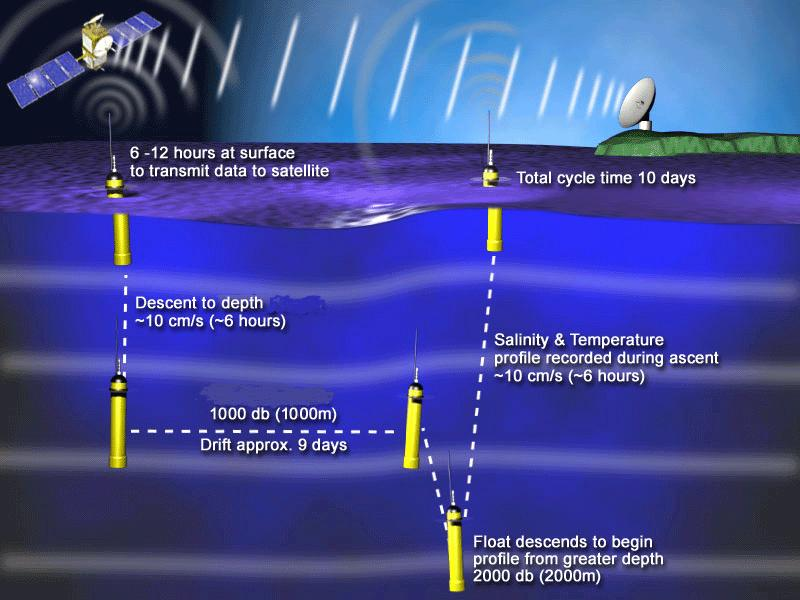
\includegraphics{pix/operation_park_profile.jpg}
        \caption[Argos Messzyklus]{Argos  Messzyklus}
        \footnotesize{
            Bildquelle: \href{https://www.csiro.au/en/Research/OandA/Areas/Marine-technologies/Argo-robotic-floats}
                        {\url{https://www.csiro.au}}
        }
        \label{fig:Argo-messzyklus}
    \end{figure}

    Die Argo Treibbojen werden mit Schiffen an spezifischen Punkten ausgesetzt. Ein Messzyklus beträgt 10 Tage. Die Boje taucht am Anfang des Zyklus auf 1000 Meter Tiefe herab.  In dieser Tiefe verbringt die Sonde die nächsten 9 Tage. Anschließend sinkt sie auf die maximale Tiefe von 2000 Metern herab, um daraufhin wieder zur Oberfläche aufzusteigen. An der Oberfläche sendet die Boje innerhalb von 6 bis 12 Stunden die Daten über den Sattelitenarray Iason an die Bodenstationen. Der oben genannte Messzyklus kann in Abbildung \ref{fig:Argo-messzyklus} nachvollzogen werden.

    \begin{figure}[!ht]
        \centering
        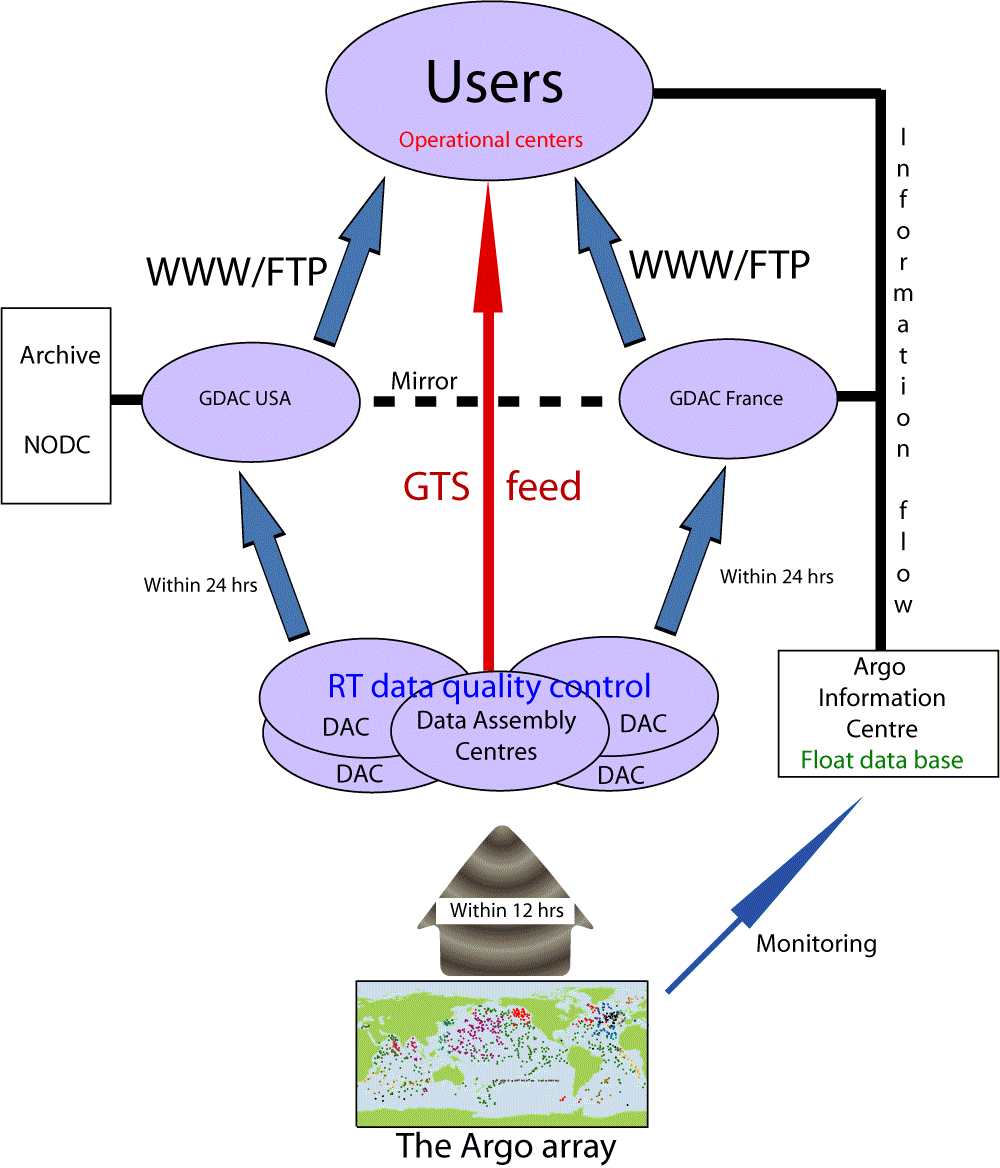
\includegraphics[width=0.4\textwidth]{pix/RT-Data-flow}
        \caption[Qualitätszyklus der Argo-Daten]{Qualitätszyklus der Argo-Daten}
        \footnotesize{
            Bildquelle: \href{http://www.argo.ucsd.edu/Argo_data_and.html}%
                        {\url{http://www.argo.ucsd.edu}}
        }


        \label{fig:argo_dataflow}
    \end{figure}

    Im Anschluss an die Erhebung werden die Daten auf deren Plausibilität und Qualität überprüft (vgl. \cite{ArgoDataBeginnersGuide} S. 3). Nach diesem Prozess werden die aufbereiteten Daten über die \gls{GDAC} in monatlichen Releasezyklen veröffentlicht. (vgl. \cite{Argofloa92:online}). Der Werdegang der Daten ist in Abbildung \ref{fig:argo_dataflow} zu sehen.

% BEGIN -- Daten
\subsection{Datengrundlage}


    Alle am Argo-Programm teilnehmenden Organisationen verpflichten sich auf eine gemeinsame Datenpolitik. So gibt es keine Herrschaft über die erhobenen Daten. Vielmehr stehen diese ab dem Zeitpunkt der Veröffentlichung transparent der Öffentlichkeit zur Verfügung.
    Nach der Übermittlung werden die Messdaten einer Qualitätskontrolle unterzogen. Sie werden auf Plausibilität und Abweichungen überprüft. Nach dieser Qualitätskontrolle werden die Daten nun über die \gls{GDAC} in Frankreich und den USA veröffentlicht. Diese können über \gls{HTTP} und \gls{FTP} abgerufen werden.

    Ein mal im Monat werden die Daten als Snapshots, unter \gls{DOI} zusammengefasst.
    Während und vor der Qualitätskontrolle liegen die Daten in den Formaten \gls{TESAC} und \gls{BUFR} vor.
    Die von den \gls{GDAC} veröffentlichten Daten liegen im Format \gls{netCDF} vor. Diese sind unter der Lizenz Attribution 4.0 International (CC BY 4.0) veröffentlicht und dürfen unter der Nennung der Lizenz frei verwendet und dabei auch verändert werden (vgl. \cite{ArgoDataDocumentation}).

% END

% BEGIN -- Datenstruktur

In Listing \ref{lst:dataOrdnerstruktur} ist die Ordnerstruktur der \gls{netCDF} Dateien zu erkennen. Über den Ordnernamen aoml ist die Herkunft des \gls{DOI} zu erkennen. In diesem Fall wurden die Dateien von einem Server der  "`Atlantic Oceanografic \& Meterolocical Laboratory"' erstellt. Hier befindet sich für jede Messboje ein Unterordner.  Die Dateien meta, prof, Rtraj und tech sind eine Quelle für Metainformationen. Die Messprofile einer Boje finden sich im Ordner \texttt{profiles}. Hier wird für jeden Messzyklus eine Datei angelegt. Dieser startet bei 1 und inkrementiert über jeden Messzyklus um 1.

    \begin{python}[label={lst:dataOrdnerstruktur}, caption={Die Verzeichnisstruktur der vom aoml bereitgestellten Daten}]
./aoml/1900200/
- 1900200_meta.nc
- 1900200_prof.nc
- 1900200_Rtraj.nc
- 1900200_tech.nc
- profiles
    - D1900200_001.nc
    ...
    - D1900200_215.nc
    - D1900200_216.nc
./aoml/1900201/
...\end{python}

% END

\subsection{Objektrelationale Unverträglichkeit}

In einem Softwareparadigma manifestiert sich ein bestimmtes Konzept in der Modellierung der Welt. Durch diese konzeptionelle Betrachtungsweise beeinflusst ein Paradigma den Erstellungsprozess sowie die Ergebnisse des Softwaredesigns und zwingt diesem seine Grenzen auf. Probleme bei der Kombination verschiedener Paradigmen werden dabei als Unverträglichkeit (impedance Mismatch) bezeichnet.
Objektorientierte Programmierung  und eine relationale Abfrage von Datensätzen sind weit verbreitete Paradigmen in der Softwareentwicklung. Damit ist die objektrelationale Unverträglichkeit eine häufig auftretende Herausforderung (vgl. \cite{ireland2009classification} S. 36-38).
Hier genannt sind unter anderem folgende Betrachtungsweisen als Ursachen für die objektrelationale Unverträglichkeit:

\begin{description}
 \item [Strukturelle Unterschiede]
 Die objektorientierte Programmierung erlaubt das Definieren beliebig komplexer Strukturen aus Methoden und Klassen. Durch Vererbungsstrukturen ist es möglich, Objekte zu spezialisieren und Grundkonzepte von Klassen zu generalisieren. Eine relationale Algebra wird durch Tupel, Mengen und Wahrheitswerte definiert. Inhärent wiederholbare Strukturen oder Hierarchien können mit diesen Mitteln nicht umgesetzt werden.

 \item [Datenkapselung]
 In der objektorientierten Programmierung können die intrinsischen Attribute eines Objektes verborgen werden. Dieses Konzept ist als Kapselung bekannt und erlaubt es, den Zugriff auf die gekapselten Strukturen einzuschränken. In einer relationalen Algebra ist eine derartige Abstraktion über die Daten nicht vorgesehen.


 \item [Objektidentität]
 Durch die Instanziierung eines Objektes aus einer Klasse erhält dieses eine eindeutige Identität. Somit unterscheiden sich zwei Objekte, auch wenn diese Träger eines identischen Datensatzes sind, durch ihre Repräsentation im Arbeitsspeicher. Relationen werden durch den Primärschlüssel, und damit über ihre Daten, definiert. Zwei eigenständige Relationen mit identischem Datensatz sind damit nicht möglich.
\end{description}


Als Hilfsmittel zur Überwindung der oben genannten Probleme werden objektrealtionale Mapper (ORM bzw. O/R-Mapper) eingesetzt. Durch dieses Mapping wird eine Schnittstelle oder Abstraktionsebene zwischen Programmteilen aus den jeweiligen Sprachparadigmen definiert, um den impedance Mismatch möglichst transparent zu überwinden.



%% TODO: Vorstellung der in SQLALCHEMY verwendeten Entwurfsmuster zur Überwindung des impedance mismatch



% BEGIN -- Geographische Informationssysteme
\subsection{Geodäsie und Kartographie}

In der vorliegenden Applikation werden geographische Daten über einen Kartendienst angezeigt. Aus diesem Grund erfolgt hier eine Zusammenfassung der wichtigsten geodätischen und kartographischen Grundlagen.


Die geographsiche Länge eines Punktes $P_l$ bezeichnet den Winkel zwischen einer vom Nullmeridian durch den Erdmittelpunkt geführten Fläche und einer Meridianebene, die durch den Punkt $P_l$ führt.
Analog dazu ist die geographische Breite eines Punktes $P_b$ der Winkel zwischen der Äquatorschnittfläche und der Flächennormalen an Punkt $P_b$ (vgl.  \cite{witte2011vermessungskunde} S. 18).
\\

Das "`World Geodetic System 1984 (WGS84)"' ist ein geozentrisches, vom Erdschwerpunkt abgeleitetes Koordinatensystem. Dieses wird unter anderem von GPS zur Zuordnung von Positionen auf der Erde verwendet. Eine schematische Darstellung ist in Abbildung \ref{fig:wgs84} zu sehen. Die  Z-Achse führt durch den Erdschwerpunkt entlang der Rotationsachse durch den Nordpol, die X-Achse vom Zentrum der Erde durch einen Nullmeridian (Greenwich) und die Y-Achse wird als Orthogonale zur X-Achse ebenso durch den Erdschwerpunkt geführt (vgl. \cite{witte2011vermessungskunde} S. 13-14).


\begin{figure}[h!]
 \centering
 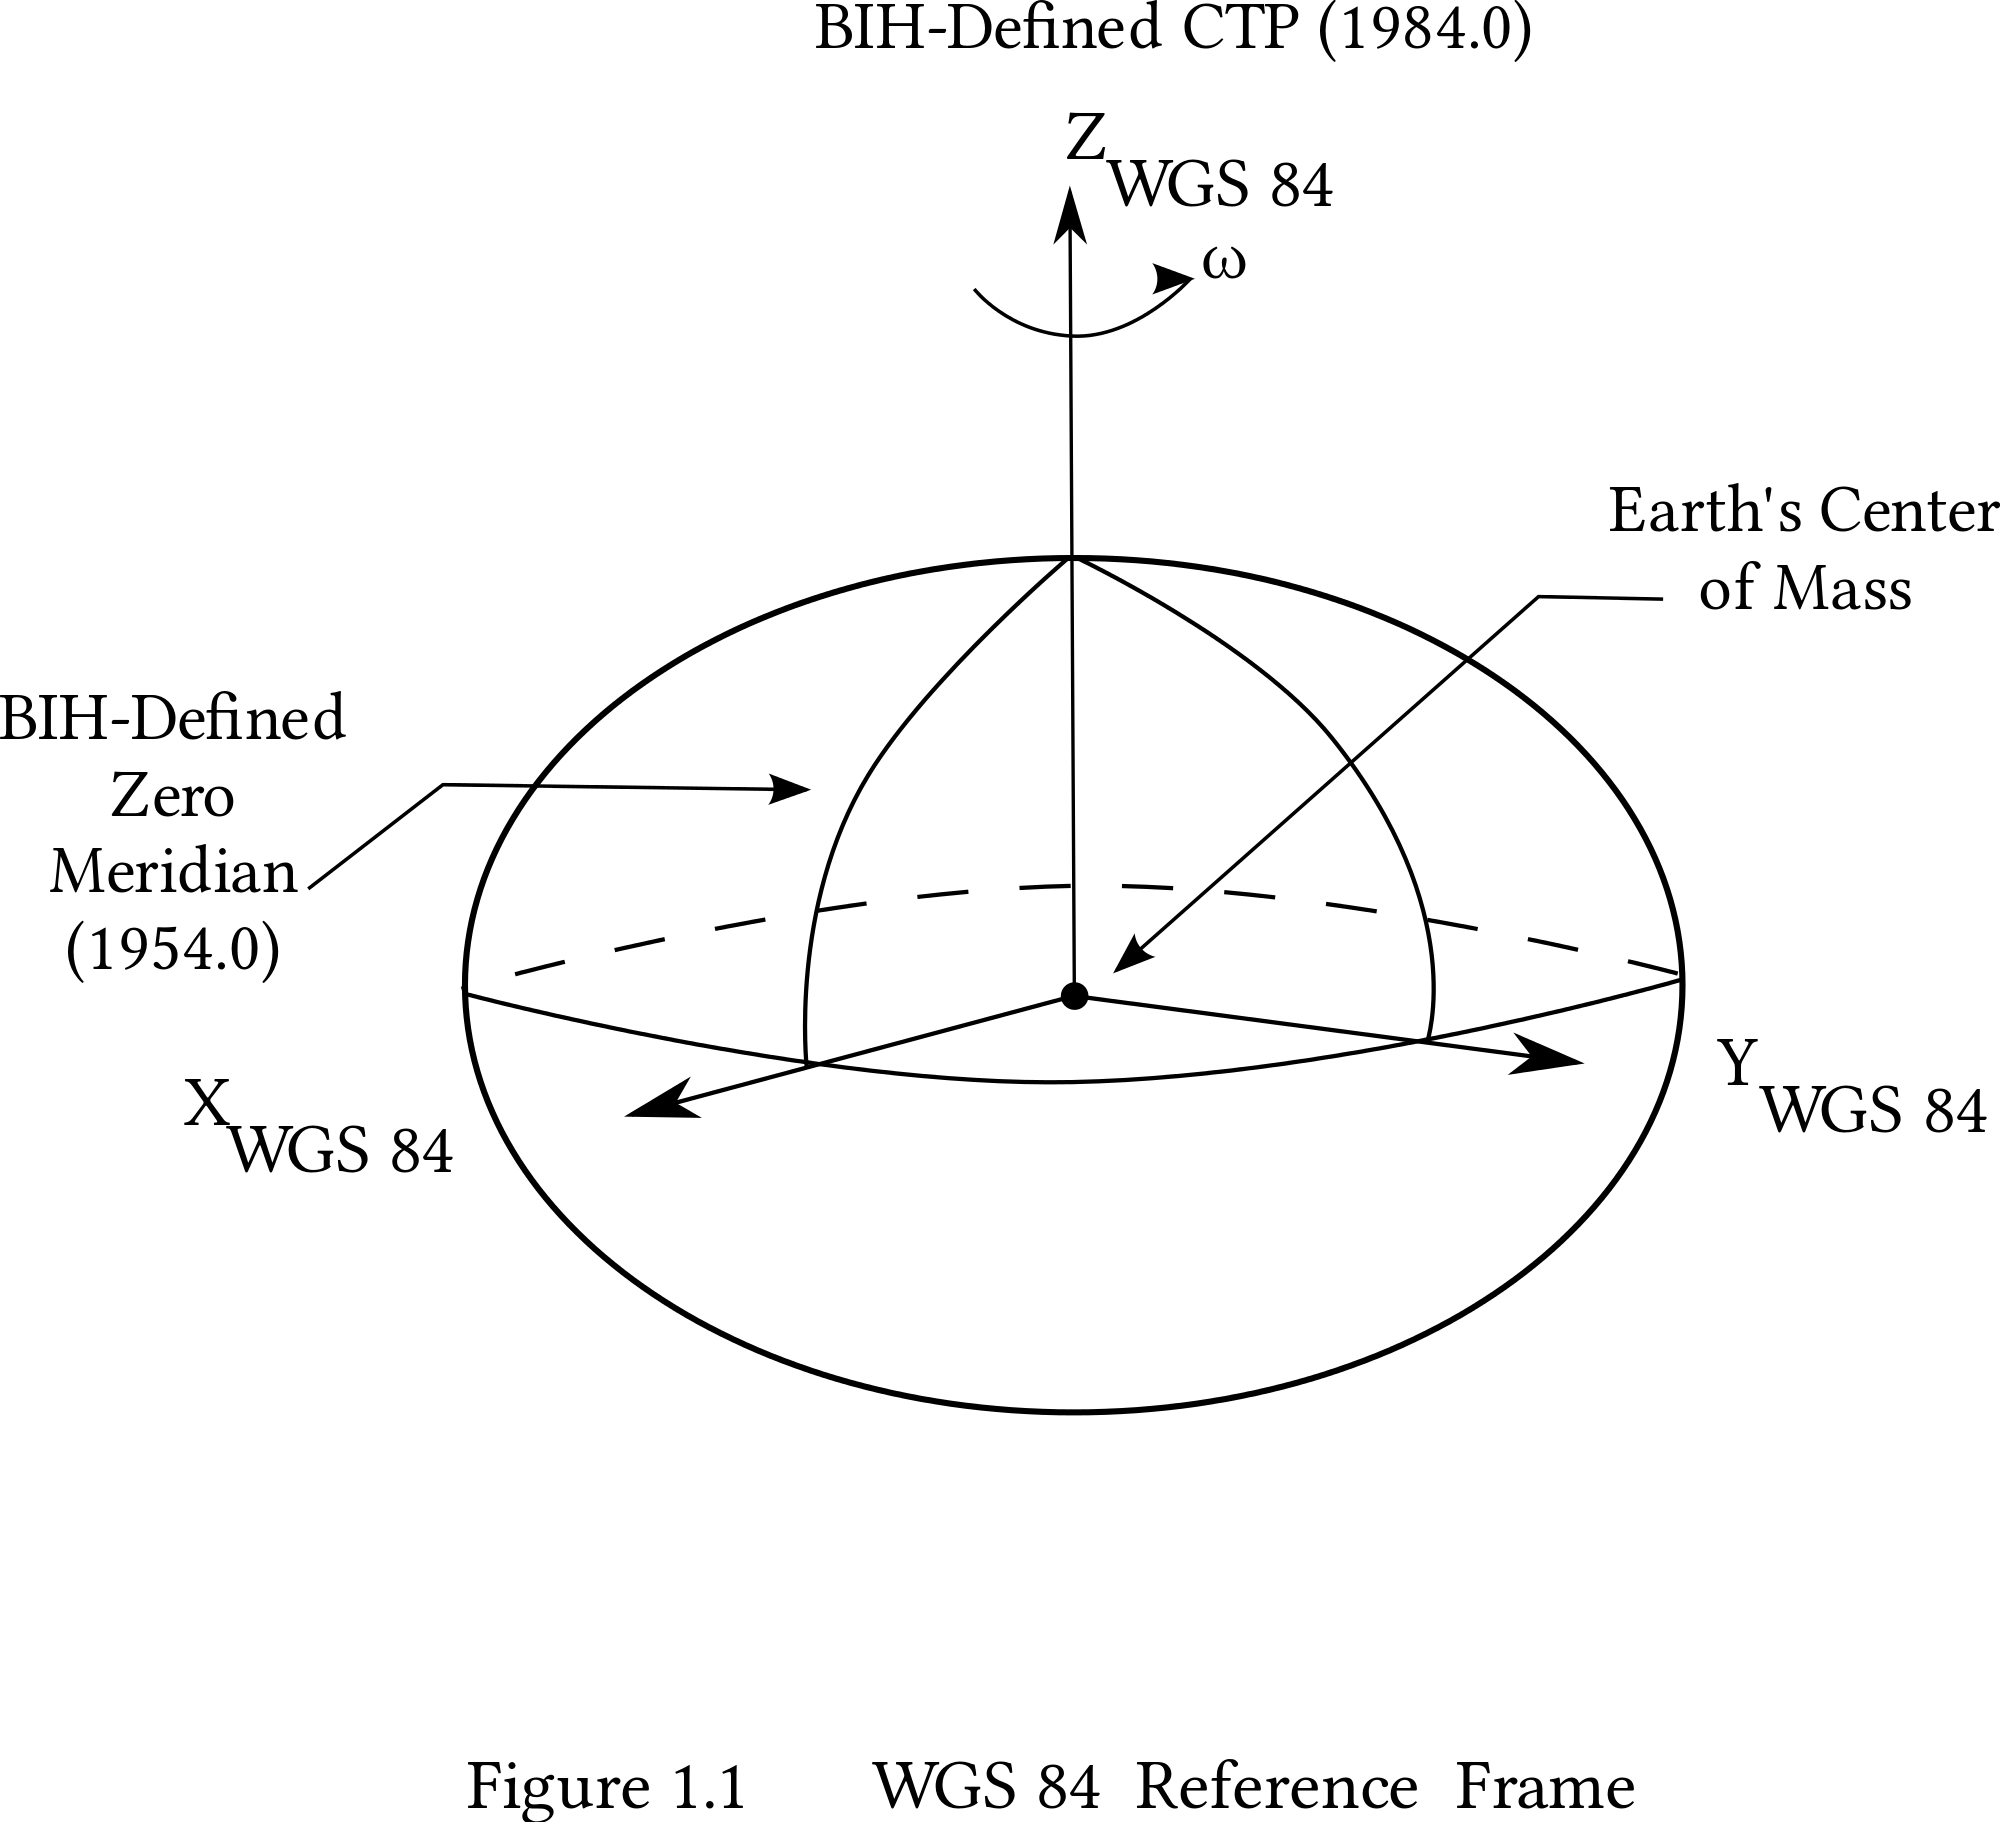
\includegraphics[width=0.3\textwidth, trim={0 9cm 0 3cm},clip]{pix/WGS_84_reference_frame.png}
 \caption[Schematische Darstellung des Koordinatensystems WGS84]
 {Schematische Darstellung des Koordinatensystems WGS84}
 \footnotesize{
    Bildquelle: \href{https://commons.wikimedia.org/wiki/File:WGS_84_reference_frame_(vector_graphic).svg}
                {\url{https://commons.wikimedia.org}}
 }
 \label{fig:wgs84}
\end{figure}



Die Gauß-Krüger Projektion erlaubt die Darstellung des Globus auf einer Ebene. Um die Krümmung des Globus auszugleichen wird die Erde in $3^\circ$ breite Meridianstreifen eingeteilt. Als Mittelpunkte dienen dabei die Meridiane $[ 3^\circ, 6^\circ, 9^\circ, \dots]$. Von den Mittelmeridianen aus wird eine Projektion an anliegende Zylinder vorgenommen. Auf diese Weise entstehen zu den Rändern der Meridianstreifen Längen- und Flächenverzerrungen, die Darstellung ist aber winkeltreu.
\\

Im UTM-System wird ein analoges Verfahren angewendet. Die Meridianstreifen haben hier aber eine Breite von $6^\circ$. Anstatt des Mittelmeridianes werden hier zwei Schnittkurven mit einem Abstand von 180km als längentreues Element für die Abbildung der Y-Achse verwendet. Der Bereich zwischen diesen Schnittkurven wird gestaucht (vgl. \cite{witte2011vermessungskunde} S. 23-25).


% END

% BEGIN -- Software
\pagebreak
    \subsection{Network Common Data Format}

    Das \gls{netCDF} dient zum Austausch von wissenschaftlichen Daten. Es ist eine Weiterentwicklung des von der NASA entwickelten \gls{CDF}. Das Datenformat zeichnet sich dadurch aus, dass es selbstbeschreibend ist. Die Dokumentation ist Teil des Datensatzes und wird so immer  mitgeführt. Dies soll die Portabilität des Datensatzes verbessern  (vgl. \cite{FishernetCDF}).

    Es wurde auch eine Bibliothek für Python entwickelt  (vgl.\cite{netCDF4}). Mit dieser ist es möglich, die Binärdaten zu öffnen und zu numpy-Arrays zu extrahieren. In Listing \ref{lst:example_netCDF} ist die Verwendung exemplarisch an der Extraktion und der Umrechnung des Erstelldatums  aufgezeigt und im Folgenden beschrieben.

    \pythonexternal[%
        % ---------------------------------------------
        %   PYTHON \gls{netCDF} als Beispiel JULD
        caption = {Extraktion eines netCDF-Datensatzes zur Berechnung des Erstellungsdatums},%
        label = {lst:example_netCDF}]%
        {scr/beispiele/netCDF_juld.py}

    Um einen Datensatz zu öffnen, bildet man eine Instanz der Klasse \texttt{netCDF4.Dataset}. Die Auswahl des Profils gelingt durch die Pfadangabe als Parameter bei der Instanzierung.
    Über das Attribut \texttt{dataset.variables} werden die Datensätze als \texttt{OrderedDict} gehalten. Bei der Extraktion eines Parameters erhält man zunächst die Dokumentation des jeweiligen Datensatzes. In diesem Fall handelt es sich um den Zeitpunkt der Sattelitenübertragung des betreffenden Messprofils.
    Aus der Dokumentation lassen sich für die Weiterverarbeitung wichtige Parameter entnehmen.
    So ist der Datensatz in Form des C-Datentyps \texttt{float64} codiert. Das Datumsformat entspricht dem \gls{Julian Day} ab dem Zeitpunkt \textit{01. Januar 1950}.

    Um die Werte eines Datensatzes zu extrahieren, wird über die numpy-slicing Operation \texttt{arr[::]} der Datensatz in vektorieller Form extrahiert. Da in diesem Array nur ein skalarer \texttt{float64} Wert enthalten ist, kann dieser als nulltes Element vom Array entnommen werden.
    Zur Überführung in das Format des Gregorianischen Kalenders wird ein Datumsobjekt des Referenzdatums benötigt. Durch die Verwendung von \texttt{timedelta} werden die Tage aus dem Feld \texttt{JULD} addiert. Da ein Messzyklus 10 Tage andauert, kann an dieser Stelle der Datensatz, durch das Überführen zu einem Integer, vereinfacht werden. Die Casting-Operation \texttt{int()} rundet in jedem Fall ab.

\section{Anforderungsanalyse}

\subsection{Systembeschreibung}

    Die zu entwickelnde Anwendung verfolgt einen datengetriebenen Ansatz. Die Daten müssen erhoben werden um diese dann über ein Webfrontend darstellbar zu machen.  Die interessierten Benutzer  können sich über die Web Präsenz die letzte Position der Bojen auf einer Karte ansehen. Durch einen Klick auf die Darstellung einer Messboje erhalten sie zudem Informationen und eine Darstellung der von dieser Messstation gemessenen Messwerte.
    
    

% BEGIN ermittlung  Anforderungen 
    \subsection{Ermittlung der Anforderungen}
    
    Ausgehend von einem ersten Prototypen  und über User-Stories wurden einige Use-Cases entwickelt \footnote{Siehe Abbildung \ref{fig:use_case}: \nameref{fig:use_case}}.  Hierbei wurden die zwei Klassen "`Benutzende"' \textbf{(B)} und "`Administrierende"'  \textbf{(A)} mit den ihnen zugehörigen Anwendungsfällen herausgearbeitet. 
    
    \begin{figure}[h!]
        \centering
        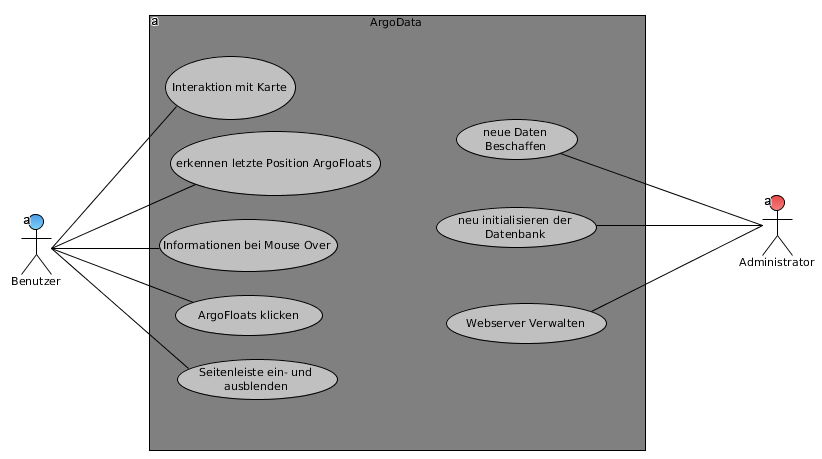
\includegraphics[width=0.8\textwidth]{pix/use-case.png}
        \caption{Use case Diagramm der Anforderungen}
        \label{fig:use_case}
    \end{figure}
    
    Anhand des so vorliegenden Modells wurde ein Abhängigkeitsgraph ausgearbeitet.\footnote{Siehe Abbildung \ref{fig:graph_anforderungen}: \nameref{fig:graph_anforderungen}}.  Dieser beschreibt die Anforderungen und deren Abhängikeiten anhand eines gerichteten Graphen. Mit hilfe dieser Darstellung konnten die Anforderungen noch feiner ausgearbeitet und um Definitionslücken erweitert werden.  
    
    \begin{figure}[h!]
    \centering
    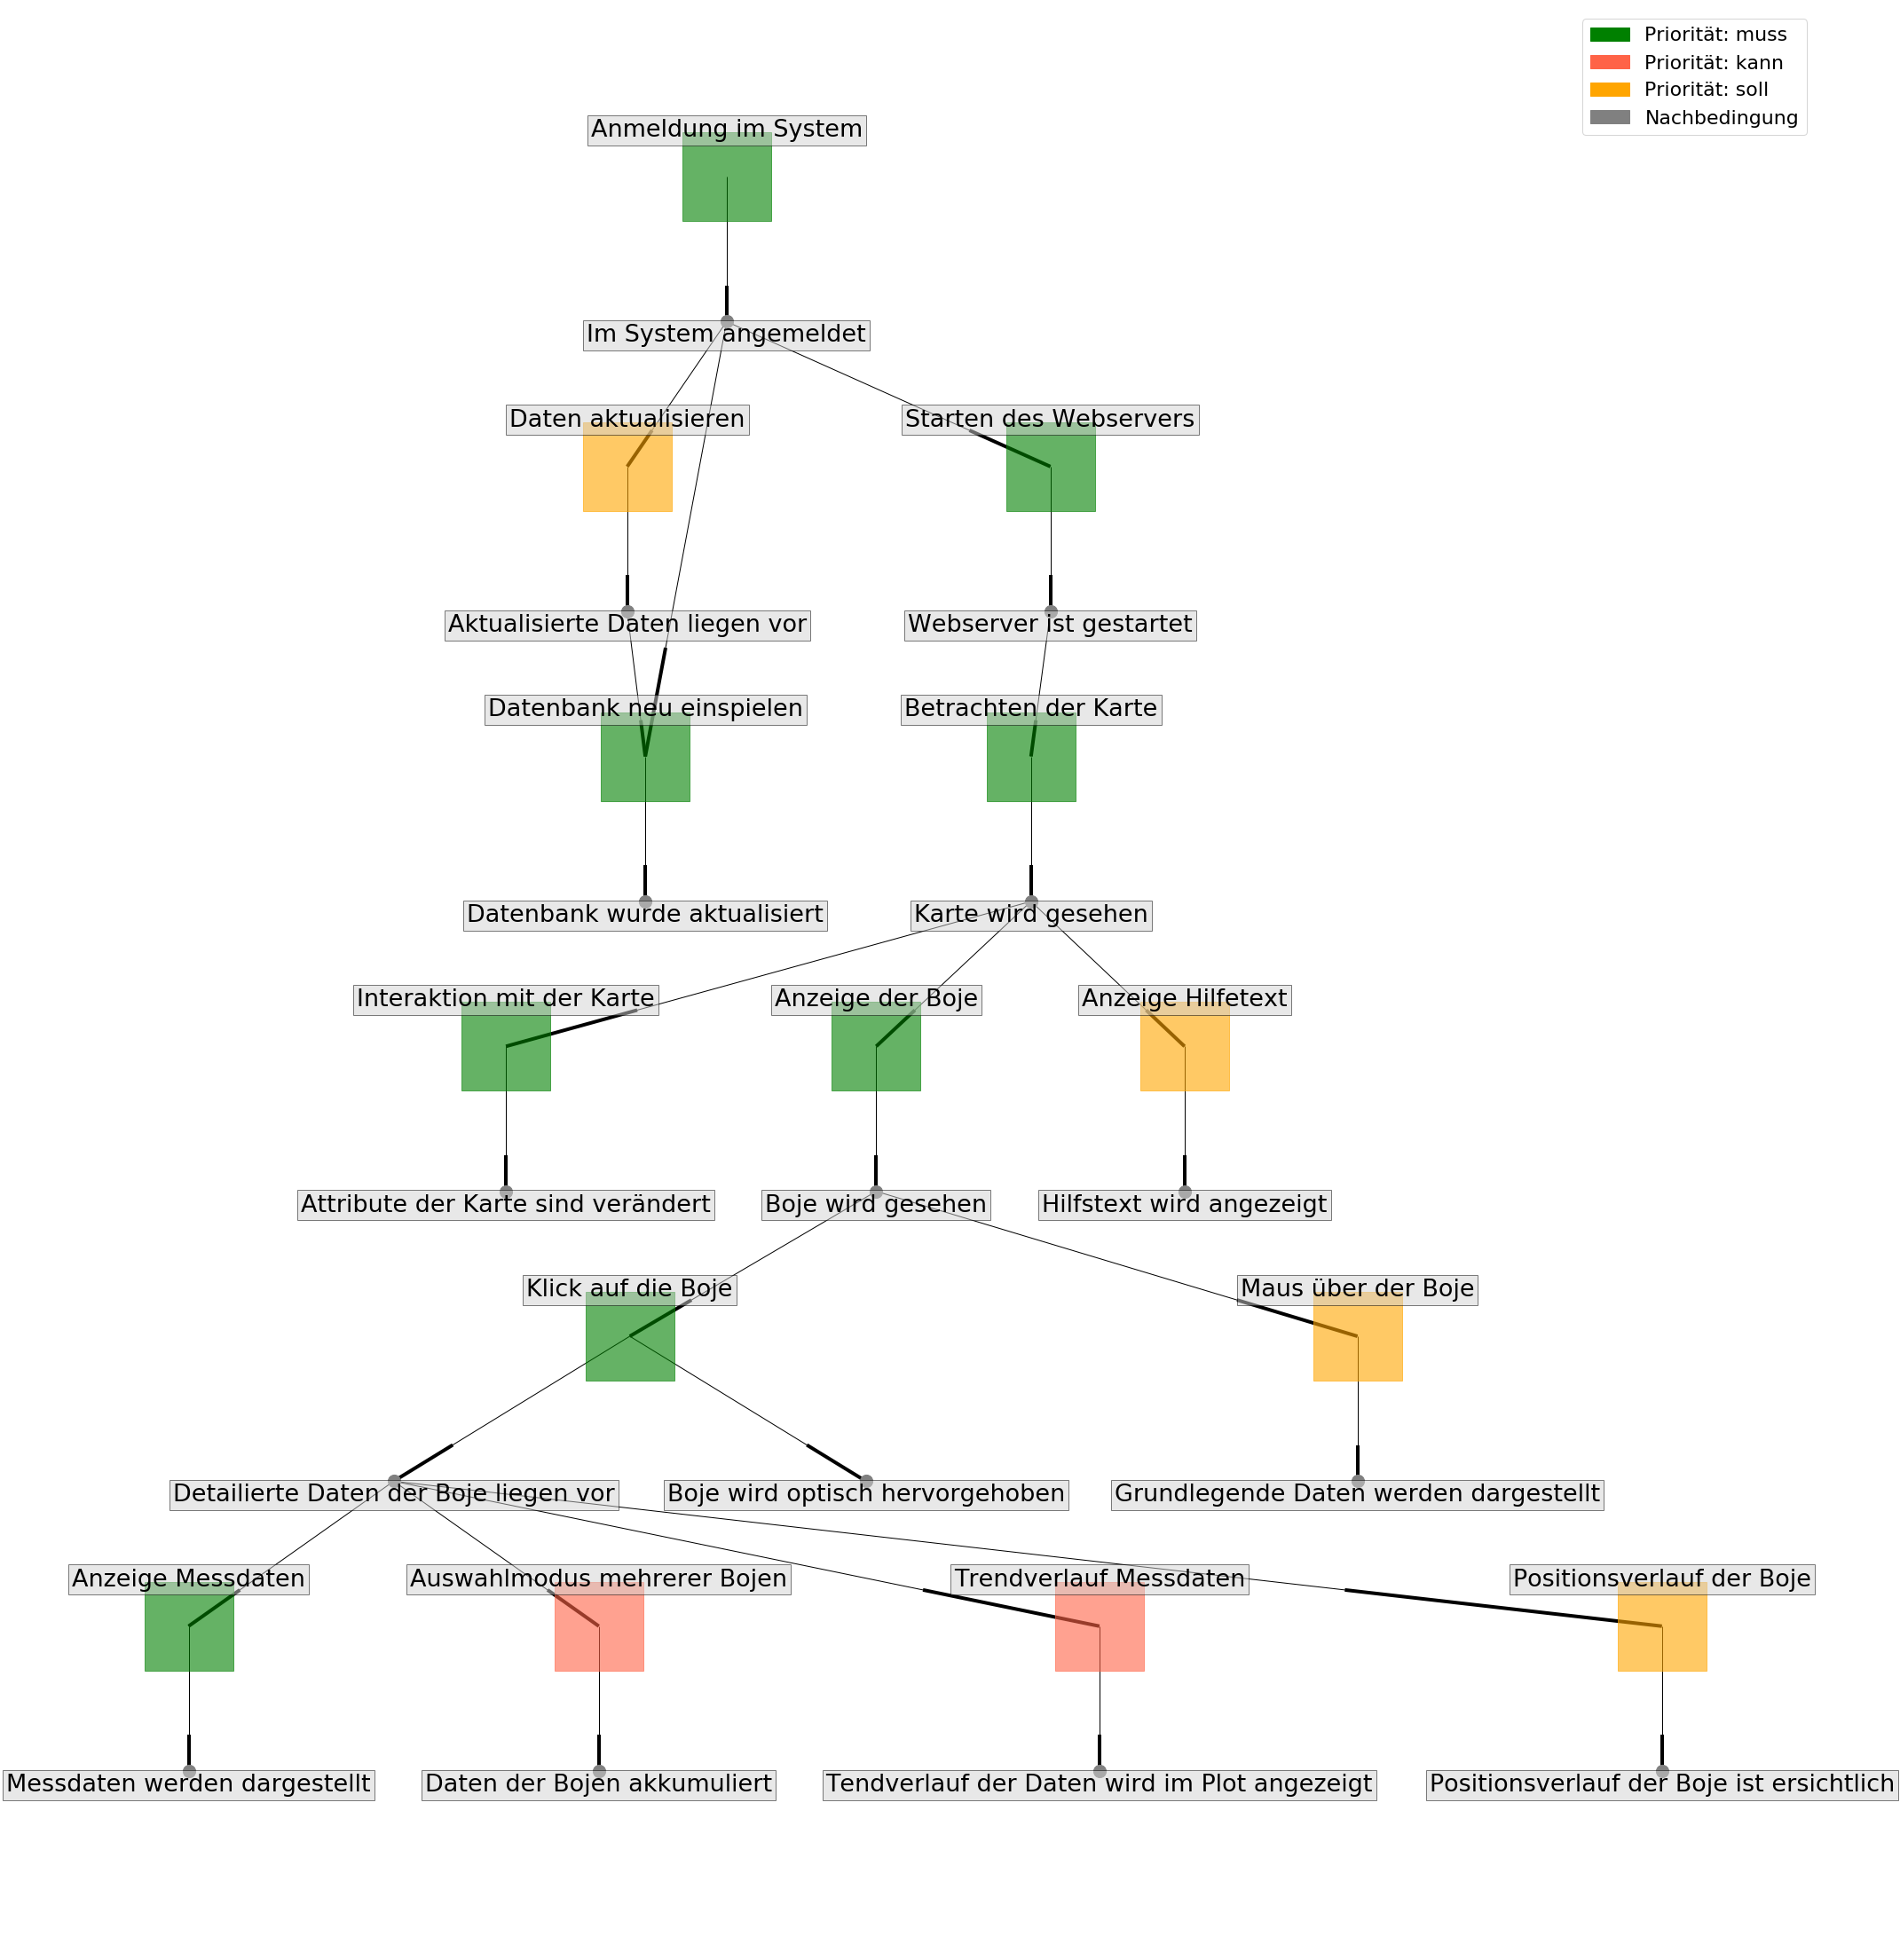
\includegraphics[width=\textwidth]{pix/graph_anforderungen.png}
    % graph_anforderungen.png: 1208x850 px, 72dpi, 42.63x29.99 cm, bb=0 0 1208 850
    \caption{Anforderungen und ihre Abhängigkeiten als gerichteter Graph}
    \label{fig:graph_anforderungen}
    \end{figure}
    
% END 
     
% BEGIN Beschreibung  funktionale Anforderungen
    \subsection{Funktionale Anforderungen}
    
    \subsubsection{Anwendende Perspektive}
    
    Die benutzenden erwarten die Darstellung einer Webapplikatin wenn diese die ihr zugehörige URL öffnen. Die Webseite soll über eine Kartenapplikation die Grenzen der Ozeane und der umliegenden Kontinente ersichtlich machen.  Eine genauere Darstellung von Landmarkern wie Straßen, Städte oder Gebirge ist für den Aussagewert der Applikation nicht erforderlich. Die Kartendarstellung soll außerdem über Interaktionsmöglichkeiten, wie dem Einstellen der Zoomstufe, sowie des ausgewählten Kartenbereichs, verfügen.
    
    Über den Kartendienst sind außerdem die letzte Position jeder Messboje aus dem Datensatz ersichtlich. Über Farbcodes wird der Status der Boje auf den ersten Blick erfahrbar gemacht. Um Streuung und Verdichtung an spezifischen Orten ersichtlich zu halten, werden alle Messstationen des angezeigten Kartenausschnittes dargestellt. Es erfolgt keine Zusammenfassung oder Ausblendung der Messstationen.
    
    Wird die Maus über eine Boje geführt, so ist es sinnvoll hier bereits grundlegende Daten der Messstation darzustellen um eine Identifikation des jeweiligen Datensatzes zu ermöglichen.
    
    Ein Mausklick auf die schematische Darstellung der Boje soll spezifischere Daten der Boje anzeigen. Dazu soll in einem separierten Darstellungsfeld, der Verlauf der Messdaten, sowie einiger weiterer sinnvoller Werte der jeweiligen Messstation angezeigt werden. Es ist sinnvoll, wenn dieser Bereich je nach Wunsch des Benutzenden zu- und wieder abgestellt werden kann. 
    
    
    \subsubsection{Administrative Perspektive}
    
    Um die Inhalte zu erstellen, werden auf Administrativer Sicht keine Journalistischen Tätigkeiten erwartet. Durch den Datengetriebenen Ansatz der Applikation müssen für das Erstellen der Inhalte keine Webmasken wie Texteingabefelder zur Verfügung gestellt werden. Vielmehr ist es hier sinnvoll, die hier benötigten Werkzeuge als Skripte zur Verfügung zu stellen, um die Administrativen Aufgaben über die Kommandozeile ausführen zu können. 
    
    Administrierende erwarten vom System dass sie neue Daten  in die Datenbank überführen können. Hierbei ist es notwendig, dass die Datensätze des Argo Programms ausgelesen und in ein für die Datenbank aufbereitetes Format überführt werden. 
    
    Es wäre sinnvoll, die Aggregation der POIs ebenfalls über einen Programmablauf zu modellieren.  In diesem Schritt müssten die Daten von der Webpräsenz des gooc heruntergeladen und an einem Ort entpackt werden. Zusätzlich müsste darauf geachtet werden, die Daten wieder zu entfernen, nachdem diese in die Datenbank des Systems überführt worden ist.
    
    Der Prozess der Beschaffung und Aktualisierung der Daten kann bis hin zur Vollautomatisierung abgebildet werden. 
% END 
    

% BEGIN Beschreibung  nicht-funktionale Anforderungen


\subsection{Nicht-Funktionale Anforderungen}
    
    \subsubsection{Anwendende Perspektive}
        Für die Benutzenden ist die Usability der wichtigste Aspekt. Die Benutzungsmuster müssen klar ersichtlich und intuitiv erfahrbar sein. Die Darstellung der Applikation soll einfach und schlicht gehalten werden und dem gewohnten Erscheinen modernen Web Applikationen entsprechen. 
        
        Es soll darauf Wert gelegt werden, die Daten möglichst schnell nach der Interaktion zu Anzeige zu bringen, da das Warten auf Webapplikationen mit Frust verbunden ist, und eine hohe Absprungrate zur Folge hätte.
        
        
    \subsubsection{Administrative Perspektive}
        Für die Aggregation der Daten ist die Sicherheit ein zentraler Aspekt. Dies umfasst sowie Aspekte von Authentifizierung und Autorisierung der Rolle der Datenaggregation als auch eine Sicherheit um die Integrität der Heruntergeladenen Daten.
    
% END 

% BEGIN Auswahl der Daten
\subsection{Benötigte Daten}

Um die Darstellung zu vereinfachen und die Kommunikation mit der Datenbank zu beschleunigen, ist im ersten Schritt eine Auswahl aus den Daten der Argo-Bojen vorzunehmen. Hierbei soll darauf geachtet werden, nur diejenigen Daten zu verwenden, welche für die Erbringung des Dienstes notwendig sind.

Aus diesem Grund findet sich im Folgenden eine Auswahl aus dem Datenkatalog \footnote{Siehe Quelle \cite{ArgoUserManual} S. 19 ff.} von Argo mit der jeweiligen Begründung:

\begin{center}
\begin{table}
  \label{table:Datenauswahl}
  \begin{tabular}{ | l | p{4cm} |p{6cm} |}
    \hline
    \textbf{Datenfeld} & \textbf{Beschreibung} & \textbf{Wird verwendet weil} \\\hline
   
    PLATFORM\_NUMBER 
        & Eindeutige Identifikationsnummer einer einer Messstation
        & Wird benötigt um Messprofile eindeutig der Plattform zuordnen zu können. \\\hline 
    
    CYCLE\_NUMBER 
        & Fortlaufende und innerhalb einer Messboje eindeutige Identifikationsnummer eines Messprofils
        & Dieser Wert wird benötigt, um Messungen eindeutig zuordnen zu können. \\\hline
    
    JULD
        & In Julian Date codierter Zeitpunkt der Übertragung (Begin oder ende?) einer Messung
        & Der Zeitpunkt wird benötigt um die Messungen in einen Zeitlichen Kontext zu stellen. \\\hline
        
    N\_PARAM
        & Anzahl der Messsensoren. 
        & Durch diesen Wert lässt sich die Anzahl der Sensoren ableiten. \\\hline
        
    LATITUDE \& LONGITUDE
        & Die Positionsdaten einer Messung zum Zeitpunkt der Übetragung der Werte.
        & Dies ist ein essentieller Parameter um die Messungen in einen lokalen Zusammenhang zu stellen. \\\hline
        
    PRES
        & Messvektor des Wasserdrucks
        & Durch diesen Messwert lässt sich die Dichte der überliegenden Wassersäule herleiten. \\\hline
        
    TEMP
        & Messvektor der Wassertemperaturen 
        &  Die Temperatur des umliegenden Wassers ist einer der zentralen Messwerte. Durch diesen Messwert und seinen Trend lässt sich der Globale Klimawandel anschaulich darstellen.  \\\hline
        
    PSAL
        & Messvektoren des Salzgehaltes
        & Ein weiterer Parameter, um die Auswirkungen des Klimawandels zu erfahren. Durch das Schmelzen der großen Eissschelfs an den Polen des Planeten ist eine Verringerung des Salzgehaltes der meere zu erwarten. \\\hline
    \end{tabular}
      \caption{Auswahl der Daten aus dem ArgoProgramm}
\end{table}
\end{center}

 

%TODO Der kleine Satz möchte aus den Untiefen der Schachtelsätze abgeholt und verbessert werden
\paragraph{Vereinfachung der Messdaten}
Die verwendeten Messwerte PRES, TEMP und PSAL eines Messprofils liegen in Vektorieller Form vor. Für die Darstellung über einen univariaten Graphen wird nur ein skalarer Wert pro Messprofil benötigt. Die Daten sollen zusammengefasst werden, bevor diese in die Datenstruktur überführt werden um die größe der Daten zu verringern. 
%TODO Implementierung welcher Algorithmus zurzusammenfassung 
 
% END 

% BEGIN technische Anforderungen
\subsection{Technische Anforderungen  }

\subsubsection{Verwendete Programmiersprachen}

Die Darstellung der Webapplikation wird mit HTML und Javascript umgesetzt werden. Diese Sprachen gelten in der Entwicklung von Webseiten als Standard und werden von den gängigen Browsern unterstützt.

Die weiteren teile der Applikation soll mit einer Sprache entwickelt werden, die alle benötigten Teilbereiche umsetzen kann.

Das \textbf{Öffnen der netCDF} Dateien und die numerische Berechnung kann mit C, Java/Scala, R und Python erfolgen. Insbesondere die beiden letzten sind in der Datenverarbeitung und Numerik als etablierte Werkzeuge zu sehen.

Die Darstellung der Seite soll durch ein Webframework unterstützt werden. Hier gibt es in beinahe allen Hochsprachen entsprechende Werkzeuge. Wählt man aus der Problemstellung der numerischen Verarbeitung R und Python heraus, so ist die Auswahl der geläufigen Webframeworks bei Python höher anzusehen. Diese Sprache besitzt eine große Anzahl von Bibliotheken für die Anbindung von Datenbanken, sowie einige etablierte Bibliotheken für die Schaffung von Webapplikationen.  

Python besitzt in Hinsicht auf Laufzeitkosten und einer nicht strikten Typisierung einige Nachteile gegenüber Sprachen wie C und Java. In Hinsicht die auf Auswahl von Programmbibliotheken, sowie der numerischen Berechnung besitzt die Sprache aber Vorteile und wird deswegen hier für die Implementierung genutzt.



\subsubsection{Server}

Für die Laufzeitumgebung der Applikation wird ein GNU/Linux eingesetzt werden. Die Software wird so entwickelt das sie unter den gängigen Distributionen lauffähig sein wird. Hier wird sich aber für Debian stable als Betriebssystem udn Laufzeitumgebung entschieden.


% ?? FOLGENDE ZEILEN NOCH VERWENDEN ??
% 
% Als Laufzeitumgebung ist ein GNU/Linux System einzusetzen. Die Aktualität der Pakete ist nicht von hoher Priorität, vielmehr sollten die bereitgestellten Programme gut getestet und stabil sein. In diesem Kontext gibt es zwei große Distributionen.
% 
% \begin{description}
%  \item [RHEL / centOS] Eine Kommerzielle Distribution und ihr freier Ableger. Von Vorteil sind hier der gute kommerzielle Support. In der Grundausstattung liefert Red Hat nur eine sehr beschränkte Paketauswahl.
%  \item [Debian] Diese Distribution besitzt eine große Community, die aktiv arbeitet und guten Support bietet. Die Paketauswahl ist sehr groß und sicherheitspatches werden schnell bereitgestellt. Mit apt und dpkg besitzt Debian einen exelenten Paketmanager. 
% \end{description}
% 
% Unter diesen Gesichtspunkten erscheint Debian als die geeignetste Distribution für dieses Projekt.

\subsubsection{Webframework}

Für Python gibt es eine große Anzahl an Werkzeugen für die Entwicklung von Webseiten. Hier werden exemplarisch 3 herausgegriffen und für die hier vorliegende Aufgabe bewertet.

\begin{description}
 \item [Django] wird beworben als \texttt{The web framework for perfectionists with dead\-lines}. Es wurde 2005 unter einer BSD Lizenz released und entwicklet, die News-Seite des \textit{Lawrence Journal-World} umzusetzen und zu verwalten. Django ist ein etabliertes und häufig verwendetes Webframework. Es ist dynamisch einsetzbar und für eine große Anzahl von Anwendungen verwendbar. Die Bibliothek ist außerdem durch Module erweiterbar. Die Software folgt dem "`\textit{batteries included}"' Ansatz und liefert in der Grundausstattung bereits alles nötige mit, um eine Webseite inklusive Login und Eingabemasken für journalistische Tätigkeiten auszubauen.
 
 \item [Flask] ist ein sogenanntes Micro-Framework. es verwendet die Toolsammlung \textit{Werkzeug} um Webseiten darstellbar zu machen. Das Farmework folgt dem KISS Ansatz und liefert im Grundumfang nur diejenigen Werkzeuge, die man für die Verwaltung von einfachen Webseiten benötigt. Die Software lässt sich über Module erweitern. Einzelne Teilprojekte von Applikationen lassen sich in sogenannte Blueprints modularisieren. 
 
 \item [Falcon] ist ebenso als Microfarmework zu sehen. Es wurde insbesondere in Hinblick auf Geschwindigkeit entwickelt. Das Framework erlaubt requests asynchron zu verarbeiten und lässt die auf Geschwindigkeit spezialisierte Python-Laufzeitumgebung pypy zu. Falcon ist ein relativ neues Framework und erfährt in letzter zeit zur Schaffung von REST-APIs immer mehr Aufmerksamkeit. Es ist aber auch möglich, mit diesem Framework Webapplikationen mit einer Anzeige über HTML-Elementen zu gestalten. 
\end{description}

In dieser Applikation wird die Schaffung von Journalistischen und redaktionellen Inhalten eine sehr geringe Rolle spielen. Unter diesem Gesichtspunkt ist die Frage der Komplexität der verwendeten Software zu klären. (..) Unter diesem Aspekt erscheint Django nicht als die ideale Wahl.

Flask und Falcon verfogen beide den Ansatz eines Microframeworks. Die Laufzeitgeschwindigkeit des Controllers erscheint an dieser Stelle nicht als limitierender Faktor der Applikation. Zwar wäre es wünschenswert, die Datenbeschaffung der Webapplikation bereits im Backend asynchron zu erledigen, doch überwiegt das breitere Spektrum an Modulen und Dokumentationen für die Webentwicklung von Flask.

Damit erscheint Flask als das geeignetste Werkzeug für diese Aufgabe.


\subsubsection{Datenbank}

Das DBMS soll über Schnittstellen in den Sourcecode des Programmes eingebunden werden. Die datenbank soll einem relationalen schema folgen. Die Verwendung sollte kostenfrei möglich sein und die benötigte Software über die Quellen des betriebssystems verfügbar sein. 

In dieser Applikation wurde sich für die Verwendung von PostgreSQL entschieden. Als Object-Realational-Mapper steht für Python SQLAlchemy zur verfügung.


% END  

\section{Systementwurf}

\subsection{Modellierung der Datenbank}

Um die Daten zu modellieren ist es sinnvoll, sich diese im Kontext der Erhebung zu betrachten. In (\ref{eq:datenstruktur}) ist dieser Prozess vereinfacht dargestellt.

\begin{equation}
    \mbox{Boje} \to (\mbox{misst}_{\mbox{an Ort}}) \to \mbox{Messprofile}\label{eq:datenstruktur}
\end{equation}

Dabei ist erkennbar, dass dieses Modell eine Verkettung von Entitäten und Ereignissen darstellt. Eine Boje misst über ihre Lebensdauer eine Anzahl von Messzyklen. Jeder dieser Messzyklen besteht aus einer gewissen Anzahl von Messwerten.

Um das Modell weiter fortzuführen, wurde diese Ereigniskette in ein Entitätsschema überführt. In Abbildung \ref{fig:ERM} ist die hier verwendete Modellierung des Prozesses zu sehen.

\begin{figure}[h!]
    \centering
    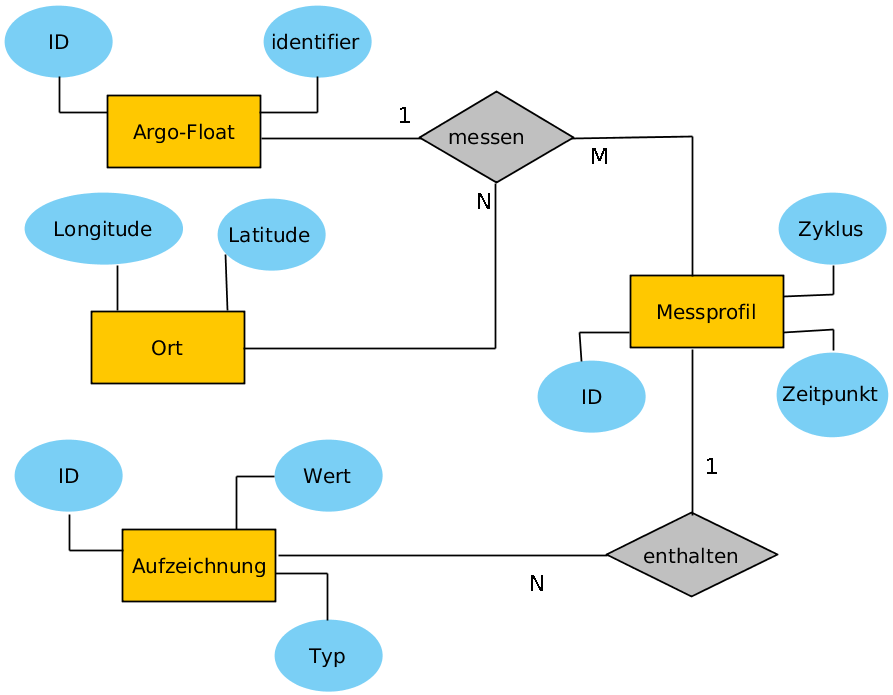
\includegraphics[width=0.6\textwidth,clip=true,trim=0pt 0pt 0pt 0pt]{pix/erm.png}
    \caption{Beschreibung der Entitäten der Datenaggregation}
    \label{fig:ERM}
\end{figure}


\subsection{Architektur}


Wie in Abbildung \ref{fig:grobetwurf_architektur_datenaggregation} zu sehen ist, besteht die Applikation aus zwei Grundkomponenten. Der erste Teilbereich ist für die Beschaffung und Aufbereitung der Daten zuständig, während der zweite Teilbereich für die Darstellung der Daten zuständig ist.

% BEGIN OOP ARCHITEKTUR   AGGREGATION
\subsubsection{Entwurf der Datenaggregation}\label{sec:entwurfAggregation}
\begin{figure}[h!]
\centering
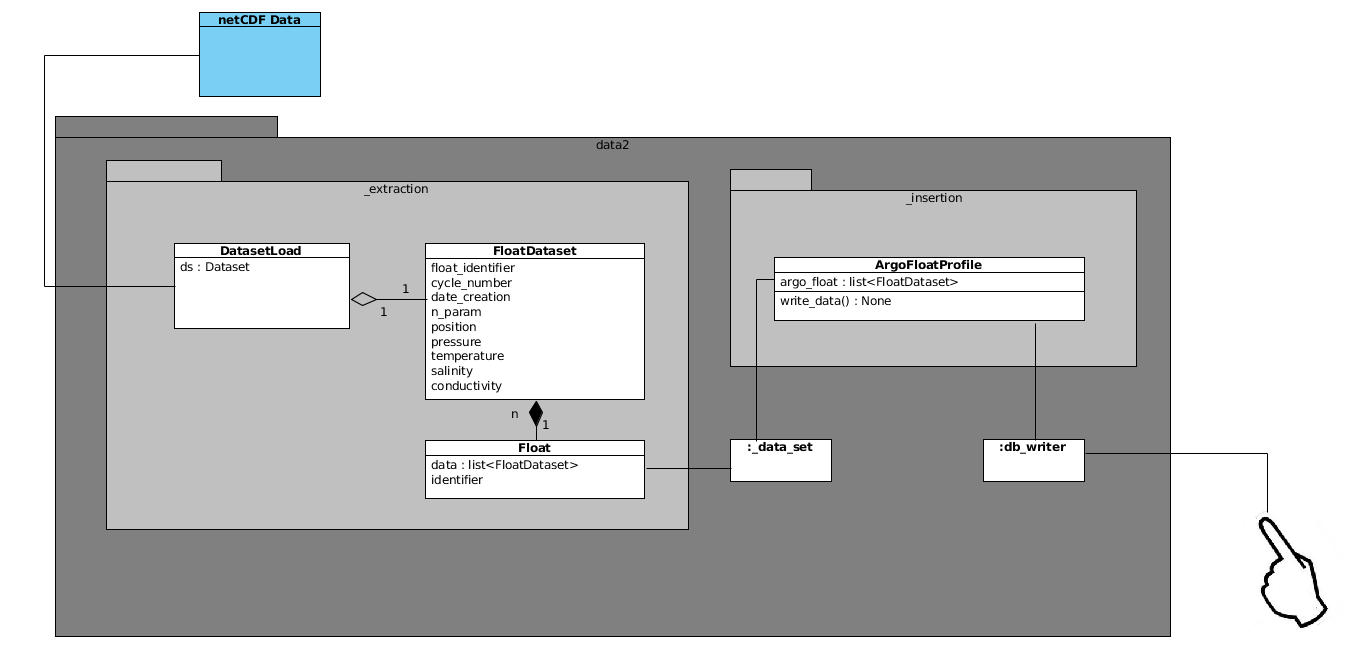
\includegraphics[width=\textwidth]{pix/grobentwurf_dataaggregation.png}
% grobentwurf_dataaggregation.png: 1436x727 px, 96dpi, 37.99x19.23 cm, bb=
\caption{Entwurf der Architektur der Aggregation der Daten}
\label{fig:grobetwurf_architektur_datenaggregation}
\end{figure}

Die Datenaggregation erfüllt zwei Funktionen. Zum einen muss sichergestellt sein, dass die Daten aus den vom Argo-Programm bereitgestellten Strukturen gelesen und in ein logisches Format überführt werden. Des Weiteren müssen diese Daten in die Datenbank der Applikation überführt werden.

Auch in diesem Modell ist die Ereigniskette aus (\ref{eq:datenstruktur}) abzubilden. Jede Messstation wird über ein Objekt abgebildet. Die hier gespeicherten Daten sind für eine Messstation eindeutig. Jeder Messzyklus der Boje wird über ein weiteres, zur Messstation gehöriges Objekt abgebildet. Dieses ist innerhalb des Kontextes eindeutig und trägt die Informationen zur jeweiligen Messung.

Für die Persistierung  werden objektorientierte Strukturen für den \gls{ORM} verwendet. Diese Strukturen teilt sich das Modul mit der Webapplikation. Die Behandlung der Daten sowie eine Steuerung des Prozesses sind als weitere Schnittstellen zu definieren.

Die Aggregation der Daten wird über zwei Teilbereiche abgebildet. Zum einen müssen die benötigten Parameter aus den Dateien ausgelesen und modelliert werden.
Als zweite Ebene der Aggregation ist der Prozess des Schreibens in eine Datenbank zu sehen. Diese verwendet die zuvor ermittelten modellierten Messprofile und schreibt sie Anhand der dort enthaltenen Daten in eine Datenbank.


Es ist an dieser Stelle zu erkennen, dass zwei Stellen existieren, die die intrinsischen Eigenschaften des Modules an dieser Stelle beeinflussen. Im folgenden werden die Schnittstellen aufgelistet, die eine richtige Handhabung festsetzen:

\pagebreak
\paragraph{Schnittstellen}

\begin{enumerate}

\item \textbf{Daten}
    \begin{enumerate}
        \item Die Datenstruktur ist normiert. Es ist sicherzustellen, dass die bekannte Daten- bzw. Ordnerstruktur abgearbeitet wird. Mit Änderungen in dieser Struktur muss nicht gerechnet werden.
        \item Es muss sicher gestellt werden, dass geöffnete Dateien wieder geschlossen werden.
    \end{enumerate}

\item \textbf{Steuerung}
    \begin{enumerate}
        \item Daten separiert in die Datenbank zu schreiben, könnte zu Inkonsistenzen führen und soll vermieden werden.
        \item Der Prozess sollte als Sequenz modelliert werden.
        \item Es muss sicher gestellt werden, dass die Daten schrittweise in die Datenbank überführt werden. Würden zu Beginn alle Dateien geöffnet und gemeinsam im flüchtigen Speicher vorgehalten, könnte es zu Problemen führen.
    \end{enumerate}

\end{enumerate}

% END

% BEGIN OOP ARCHITEKTUR   WEBAPPLIKATION

\subsubsection{Entwurf der Webapplikation}

Die Webapplikation besteht aus zwei Teilkomponenten. Die erste Komponente ist für die Darstellung der Webseite zuständig (app). Durch diese werden Elemente in  HTML, Javascript und als Bilder ausgeliefert, welche im Webbrowser den Benutzenden angezeigt werden können. Die Darstellung erfolgt dabei dem Singlepage-Prinzip.

Die zweite Teilkomponente ist dafür zuständig, benötigten Daten bereitzustellen (api). Alle Daten aus der Datenhaltung werden über diese Schnittstelle angefordert. Die Daten werden über JSON codiert.


\subsubsection{Ausarbeitung der Webrouten} \label{sec:entwurfRoutes}


Die \textbf{api} ist dafür zuständig, die benötigten Daten der Applikation bereitzustellen. Über definierte Webrouten wird über einen GET-Request ein JSON angefordert. Die  hierfür ausgearbeitete Struktur ist in Listing \ref{lst:routesAPI} zu sehen und ist im Folgenden beschrieben:

\begin{python}[label={lst:routesAPI}, caption={Webrouten der Datenrepresentation}]
(1.1) GET     /last_seen
(1.2) GET     /last_seen/[force_reload]
(1.3) GET     /argo_float/[identifier]
(1.4) GET     /positions/[identifier]
\end{python}

\begin{description}
 \item [(1.1) / (1.2)]
    Über diese Route  werden die Daten für die letzte Position der Messstationen aufgerufen. Dieser Datensatz trägt die Daten, die zur Anzeige der Positionen der Messstationen auf der Weltkarte benötigt werden und die Zusatzinformationen zur Darstellung eines Tooltips der einzelnen Argo-Floats. Die Daten werden bei jedem Besuch der Webseite ausgeliefert. Da sich diese erst verändern, wenn neue Daten vorliegen, werden diese über einen Caching-Mechanismus vorgehalten. Der optionale Übergabeparameter \texttt{force\_reload} ermöglicht das Neuanlegen des Caches. Um Vandalismus vorzubeugen, sollte es sich dabei um einen nicht zu  erratenden Token handeln.

 \item [(1.3)]
    Über diese Route werden die Mess-, wie auch Metadaten einer Messstation angefordert. Die Auswahl der Boje erfolgt über den Übergabeparameter \texttt{identifier}. Hier wird die eindeutige Identifikationsnummer  (siehe PLATTFORM\_NUMBER in Tabelle \ref{table:Datenauswahl}) der Messstation verwendet.

 \item [(1.4)]
    Um den Positionsverlauf einer Boje anzufordern, dient diese Route. Auch hier wird zur Identifikation der Messstation deren Identifikationsnummer als Parameter übergeben.
\end{description}



Die \textbf{app} liefert die Teile aus, die vom Benutzer gesehen werden. Es handelt sich dabei um HTML/Javascript und Bilddaten. Die hierfür ausgearbeitete Struktur ist in Listing \ref{lst:routesAPP} zu sehen und im Folgenden beschrieben:

\begin{python}[label={lst:routesAPP}, caption={Webrouten der Darstellung}]
(2.1) GET     /
(2.2) GET     /chart/[identifier]
(2.3) GET     /info/[identifier]
\end{python}

\begin{description}
 \item [(2.1)]
 Über diese Seite ist die eigentliche Applikation zu sehen. Dies umfasst die Karte sowie die angezeigten Messwerte.

 \item [(2.2)]
 Diese Route stellt den Plot der darzustellenden Messwerte als Bild zur Verfügung.

 \item [(2.3)]
 Über diese Route wird ein \gls{HTML} für die Infoanzeige einer Messstation bereitgestellt.

\end{description}


% END
\pagebreak
% BEGIN DESIGN DARSTELLUNG
\subsubsection{Aussehen der Webapplikation}
%
%
% - Darstellung der Daten -- ...

\begin{figure}[h!]
    \centering
    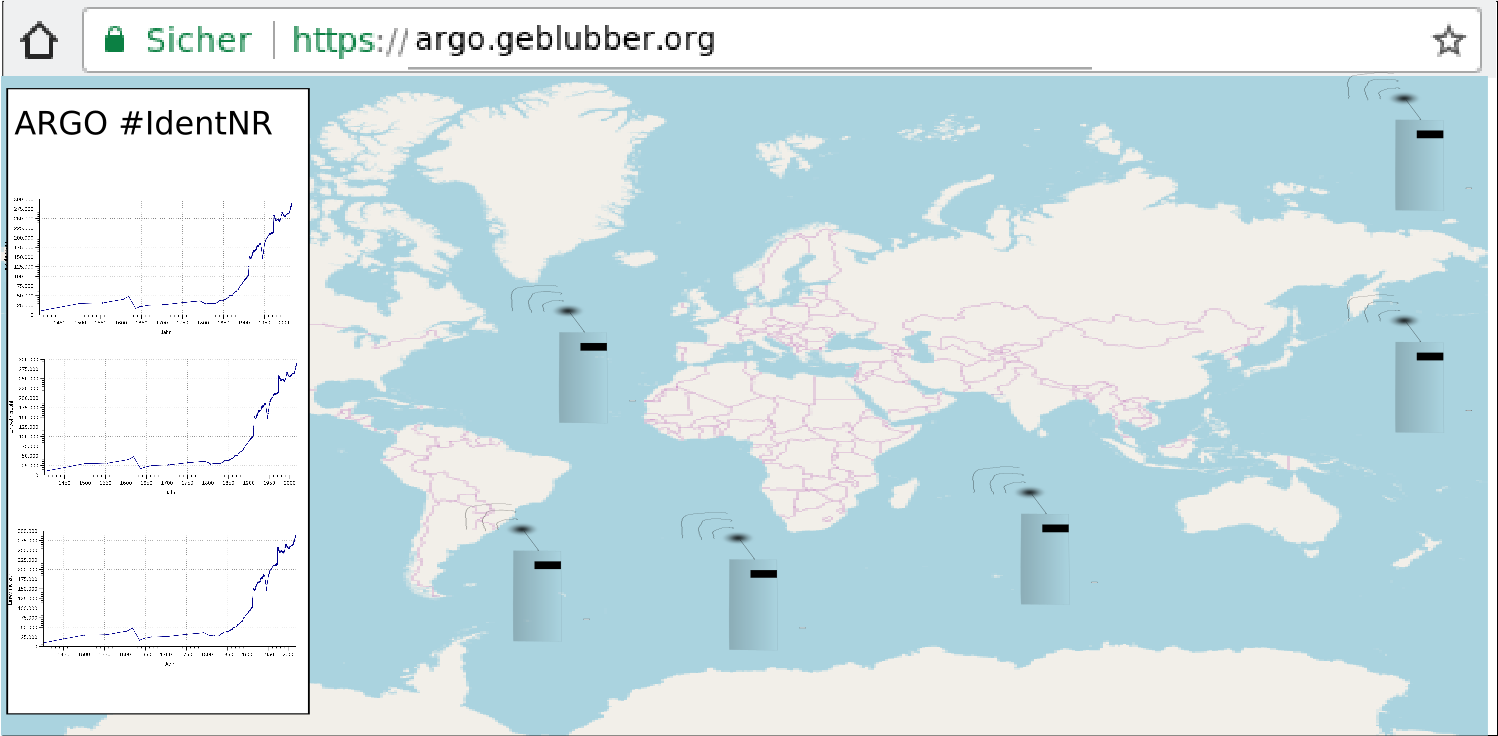
\includegraphics[width=\textwidth]{pix/EntwurfWebseite.png}
    % Entwurf_Webseite.svg.png: 1498x736 px, 96dpi, 39.63x19.47 cm, bb=0 0 1123 552
    \caption{Grafischer Grobentwurf der Webapplikation}
    \label{fig:entwurf_webseite}
\end{figure}

Das Aussehen der Applikation soll dem Muster von gängigen Webapplikationen entsprechen. In Abbildung \ref{fig:entwurf_webseite} ist ein erster Grobentwurf der Applikation zu sehen.
Zentrales Element der Applikation ist die Darstellung einer Karte. Über diese sollen die letzten Positionen der Karte ersichtlich sein.
Klickt man eine Messstation an, so wird auf der linken Seite ein weiteres Element in die Seite eingefügt. Dieses dient zur Darstellung der Messwerte des jeweiligen Argo-Floats.





% END

\section{Implementierung}

\begin{figure}[h]
 \centering
 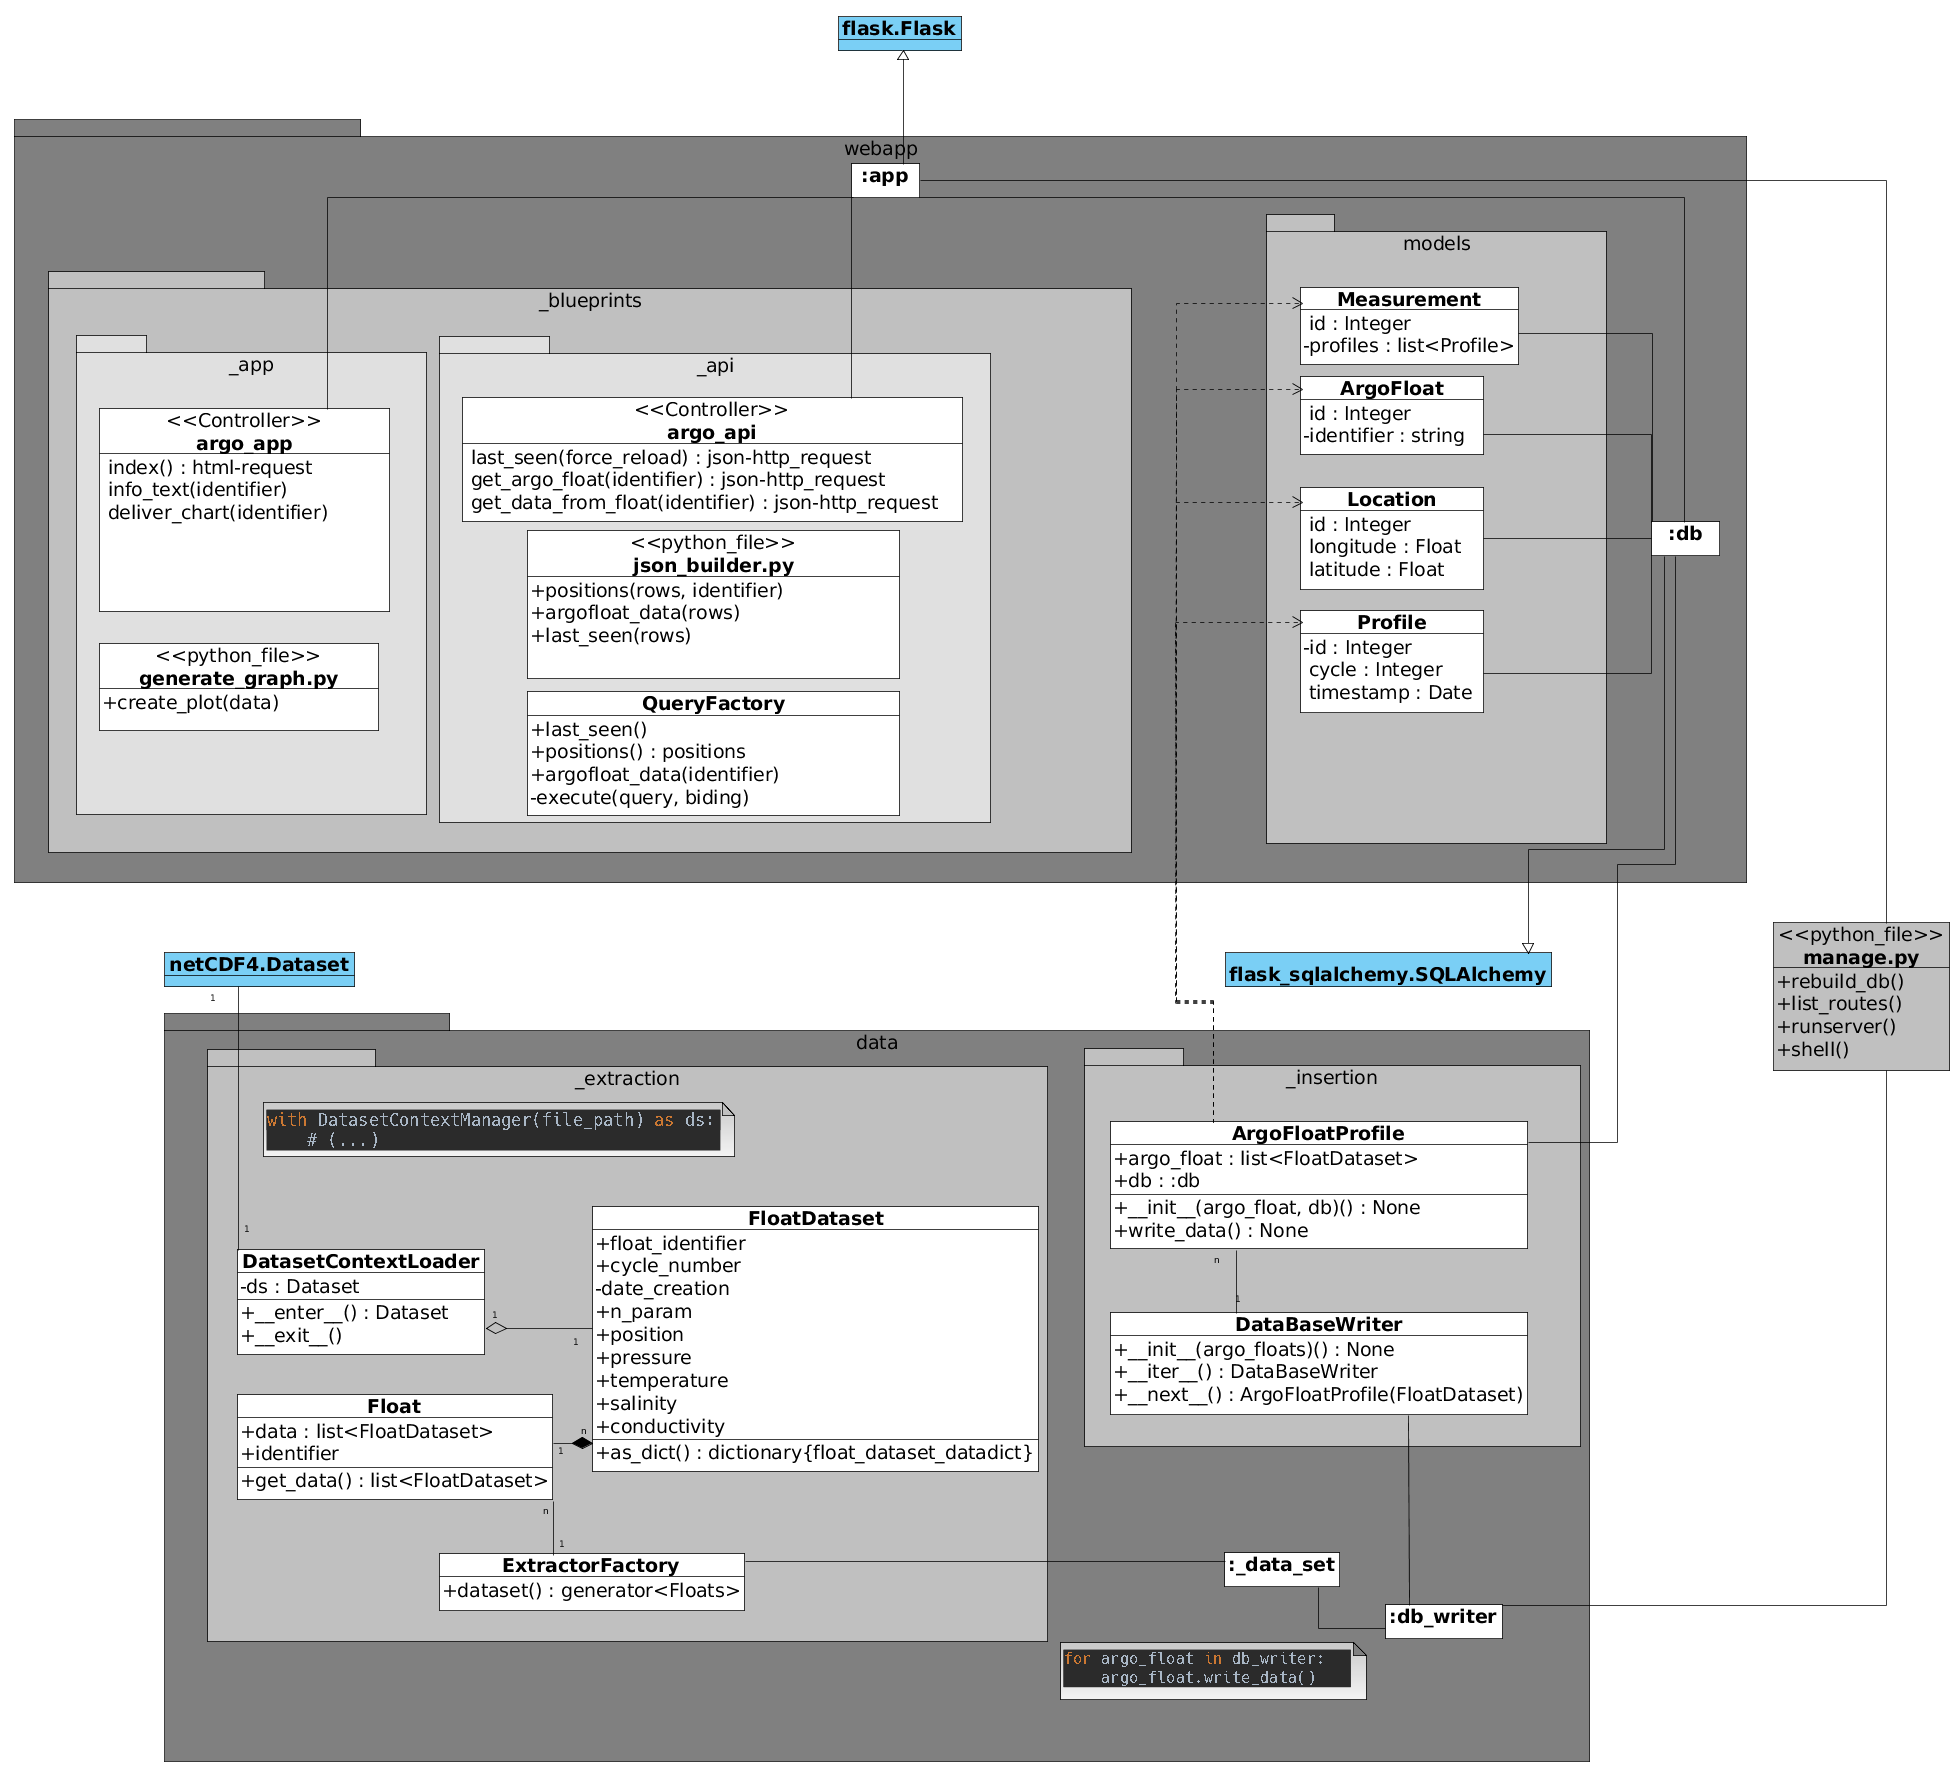
\includegraphics[width=\textwidth]{pix/Modulschema_komplett.png}
 % Modulschema_komplett.png: 876x911 px, 96dpi, 23.17x24.10 cm, bb=0 0 657 683
 \caption{Architekturbeschreibung von ArgoData}
 \label{fig:modulschema}
\end{figure}


% BEGIN DatenAGGREGATION
\subsection{Datenaggregation}


\subsubsection{Auslesen der Daten}

Der Datensatz besteht vor der Verarbeitung aus einer Ansammlung von Verzeichnissen und Dateien. Da die Gefahr besteht, dass geöffnete Dateien nicht wieder ordnungsgemäß geschlossen werden, muss eine Schnittstelle geschaffen werden, die unsachgemäße Verwendung der Dateien verhindert. Python sieht für diesen Zweck den Kontextmanager vor. In Listing \ref{lst:contextmanager} ist die hier verwendete Implementierung zu sehen.
\pagebreak
\pythonexternal[%
        caption={Kontextmanager zur Sicherstellung der richtigen Dateibehandlung.},
        label=lst:contextmanager]{./scr/beispiele/contextmanager.py}

In Listing \ref{lst:verwendungcontextmanager} ist die Verwendung des Kontextmanagers aufgezeigt und im Folgenden beschrieben.

\begin{python}[%
caption={Die Verwendung des Kontextmanagers},%
label={lst:verwendungcontextmanager}]
with DatasetContextManager(file_path) as ds:
    juld = ds.variables['JULD'][0]
\end{python}


Durch die Verwendung der Struktur über das Schlüsselwort \texttt{with} wird die Objektmethode \texttt{\_\_enter\_\_} aufgerufen. Diese gibt den objekteigenen \gls{netCDF}-Datensatz zurück. Dieses wird in der Verwendung im gleichnamigen Objekt \texttt{ds} gespeichert. Im darauf folgenden Operationsblock kann das Objekt nun verwendet und dessen Daten extrahiert werden. Nachdem der Operationsblock verlassen wurde, wird die Methode \texttt{\_\_exit\_\_} des Kontextmanagers aufgerufen. Innerhalb dieser Methode wird die Datei nun geschlossen.  Durch dieses Entwurfsmuster ist die richtige Verwendung der Datei also transparent sichergestellt. Ein Entwickler kann somit nicht durch Unachtsamkeit vergessen, den Datensatz zu schließen. Gleichzeitig erhöht sich die Lesbarkeit. Durch den Operationsblock ist jederzeit ersichtlich, ab welcher Stelle im Quelltext der Datensatz nicht mehr verfügbar ist.
Diese Schnittstelle wird in den Objektrepräsentationen der Argo-Floats und der Datensätzen verwendet, um auf die Daten zuzugreifen. In diesen wird die in Kapitel \ref{sec:entwurfAggregation} gezeigte Datenstruktur vorgehalten.


\subsubsection{Schreiben der Daten}

Um die Verarbeitung der Daten sowie den Prozess der Aggregation in der Datenbank richtig zu modellieren, ist es sinnvoll, den Prozess als Sequenz zu modellieren. Dies erlaubt es, die Datenstruktur über einen Generator vorzuhalten. Python sieht dafür den Iterator vor.
Die hier verwendete Implementierung ist in Listing \ref{lst:iteratorimpl} zu sehen. Das Interface wird über die Funktion \pythoninline{def __next__(self)} realisiert.
Dieses delegiert die Iteration zum Objekteigenen Generator \pythoninline{self.argo_floats}. In dem Moment, in dem ein Objekt aus dem Generator angefordert wird, findet die Verarbeitung der Datenstruktur statt.
Zum Schluss wird der Datensatz über ein Objekt ausgeliefert, das es erlaubt, die Daten in die Datenbank zu überführen.
Damit ist sichergestellt, dass der Prozess nur als Sequenz verwendet werden kann.

\pythonexternal[%
        caption={Implementierung des Iterators zur Steuerung der Aggregationssequenz}, label={lst:iteratorimpl}]{../BA_argo_proto/data/_insertion/_database_writer.py}

Die Verwendung der Schnittstelle ist in Listing \ref{lst:iterator_verwendung} aufgezeigt.

\pythonexternal[%
        caption={Verwendung der Schnittstelle zur Steuerung der Datenaggregation},
        label = {lst:iterator_verwendung}]{./scr/beispiele/lst-iterator-verwendung.py}



Eine zentrale Problemstellung im Prozess der Überführung der Daten in das relationale Schema ist die effektive Verwendung des flüchtigen Speichers. Eine klassische, sequenzielle Verarbeitung würde die Daten initial auslesen und diese in Gänze im Arbeitsspeicher vorhalten, bevor diese über den Mapper in die Datenbank überführt werden. Dieser Prozess wurde hier durch die Verwendung von Generatoren aufgebrochen. In Listing \ref{lst:dataextractor} ist die Implementierung dieser Schnittstelle zu sehen. Da in der Comprehension runde statt eckige Klammern verwendet werden, wird initial nur die logische Struktur als Sequenz vorgehalten. Die inhärenten Float-Objekte des Generators werden zu dem Zeitpunkt erzeugt, wenn diese durch eine Iteration aufgerufen werden. Damit werden die Daten erst zu dem Zeitpunkt ausgelesen, wenn diese für die weitere Verarbeitung benötigt werden.



Die Methode \texttt{get\_data\_sets()} erzeugt aus jedem Unterordner im definierten Arbeitsverzeichnis ein Float-Objekt und gibt dieses über das Schlüsselwort \texttt{yield} zurück. Durch diese Klasse wird somit ein Generator definiert, der es erlaubt, alle im Arbeitsverzeichnis definierten Argo-Float-Datenobjekte bereitzustellen, ohne diese bereits bei der Instantiierung kennen und abarbeiten zu müssen.


\pythonexternal[caption={Factory zur Extraktion der Datensätze},
                label={lst:dataextractor}]{/home/sebsch/Dokumente/Uni-Workdir/Bachelorarbeit/BA_argo_proto/data/_extraction/_data_extractor.py}




%END

\pagebreak
% BEGIN Webapp
\subsection{Webapplikation}

\subsubsection{Objektrelationales Mapping}\label{sec:implementierungORM}

% 1. Vorstellung SQL-Alchemy -- warum gewählt; Vor- und Nachteile

Als Objektrelationalen Mapper wird SQLAlchemy eingesetzt. Diese Software gilt als erprobt und wird bereits in einer Vielzahl von Softwaresystemen eingesetzt. So verwendet unter anderem reddit oder die Mozilla Foundation SQLAlchemy als Schnittstelle zur Datenhaltung. SQLAlchemy wird für die Verwendung in Flask empfohlen und es existiert eine Erweiterung, um die Verwendung des Mappers in Flask zu vereinfachen (vgl. \cite{openingtheflask} S. 33). \\
%% TODO Konzepte, Pattern und Nachteile von SQLAlchemy -- Pattern in Grundlagen zu ORM
%           1. LazyLoading
%           2. databinding
%           3. Foreign Key Mapping
%           4. rollback


% 2. Implementierung von Entitäten, und Relationen
In SQLAlchemy werden die Tabelleneinträge in Modellklassen abgebildet. In Listing \ref{lst:models_argofloat} ist die Implementierung des Models für eine ArgoFloat-Messstation zu sehen.

\pythonexternal[%                       -> SQLALCHEMY: ArgoFloat
    caption={Modellklasse für ein Argo-Float},%
    label={lst:models_argofloat}]%
    {/home/sebsch/Dokumente/Uni-Workdir/Bachelorarbeit/BA_argo_proto/webapp/models/_argo_float.py}

Die Registrierung des Models erfolgt über die Vererbung der Metaklasse \texttt{db.Model}. Die Eigenschaften der jeweiligen Entitäten werden über Attribute des Objektes implementiert. Diese werden in Instanzen von \texttt{db.Column} transferiert. Dies erlaubt das Festsetzen des Datentyps. So lassen sich auch weitere Datenspezifikionen definieren.  Die Attribute werden durch eine Parameterübergabe in den Initiator der Klasse mit Werten versehen.
Um das Binding umzusetzen, wurden Nachfahren der Modellklassen erzeugt. Diese benötigen für die Zuordnung das Attribut \texttt{\_\_bind\_key\_\_}.

Über das Schlüsselwort \texttt{db.relationship} werden Beziehungen beschrieben. In diesem Fall besteht eine $1 - N$ Beziehung  zu \texttt{measurements}($\mbox{argo\_float} \leftarrow \mbox{measurements}$)   (siehe auch Abbildung \ref{fig:ERM}). Als Übergabeparameter wird ein Name für die Beziehung erwartet. Der Parameter \texttt{backref} gibt den Namen der Klasse auf dem Mapper an. Diese Einstellung erlaubt den Aufruf der Beziehung auch in die entgegengesetzte Richtung. Der Parameter \texttt{lazy} definiert die verwendete Strategie für das Lazyloading. In diesem Fall wurde sich für \texttt{'dynamic'} entschieden. Diese Einstellung gibt bei Lesezugriffen ein vorkonfiguriertes Query-Objekt zurück. Dies erlaubt das Hinzufügen weiterer Filter vor dem Zugriff auf die Tabellen. Die durch diese Beziehung verbundene Modellklasse Measurements ist in Listing \ref{lst:models_measurement} zu sehen.

\pythonexternal[%                       -> SQLALCHEMY: measurement
    caption={Modellklasse für eine Messung},%
    label={lst:models_measurement}]%
    {/home/sebsch/Dokumente/Uni-Workdir/Bachelorarbeit/BA_argo_proto/webapp/models/_measurement.py}

Auf dieser Seite der Beziehung   $\left( \mbox{measurement} \to \mbox{argo\_float} \right)$ unterscheidet sich deren Implementierung. Für die eindeutige Zuordnung des übergeordneten Argo-Floats wird deren \texttt{id} als Fremdschlüssel registriert. Die Beziehung benötigt neben dem Namen der anderen Seite keine weiteren Parameter, da die Beziehung bereits konfiguriert worden ist.


% 3. Lesen und schreiben von Daten aus der Datenbank -- Rollbacks


Das Schreiben von Daten über den Mapper SQLAlchemy ist Teil der Datenaggregation. Der dort implementierte Programmcode ist in Listing \ref{lst:sqlalchemy_write} zu sehen.


\pythonexternal[%                       -> SQLALCHEMY: Schreiben
    caption={Das Schreiben der Daten eines Argo-Floats in die Datenbank},%
    label={lst:sqlalchemy_write}]%
    {/home/sebsch/Dokumente/Uni-Workdir/Bachelorarbeit/BA_argo_proto/data/_insertion/_argo_float_profile_writer.py}


Die hier implementierte Klasse \texttt{ArgoFloatProfile} ist für das Schreiben aller Datensätze eines ArgoFloats zuständig. Diese verwendet für die Zuordnung der Daten die Modell-Klassen aus der Webapplikation. Durch die Methode \texttt{write\_data} werden die Daten des durch \texttt{\_\_init\_\_} übergebenen Datensatzes in die Datenbank überführt.
Um ein dynamisches Binding realisieren zu können, wird der betreffende Parameter \texttt{bind} übergeben. Mithilfe dieses Parameters wird eine Session aufgebaut, welcher das Schreiben in die Datenbank erlaubt, die über das Binding definiert ist.

Für jeden Datensatz wird eine Instanz der betreffenden Modell-Klasse erstellt. Die dafür benötigten Daten werden aus den Datensätzen des Klasseneigenen Generator-Objektes \texttt{argo\_float} angefordert und als Parameter übergeben.

Der zuvor definierten Session werden nur die Instanzen der \texttt{Profile}-Klassen übergeben. Da alle zum Messprofil gehörenden Modells in diesem Kontext eindeutig sind, kann SQLAlchemy diese selbstständig zuordnen.
Zum Abschluss werden die Daten über \pythoninline{session.commit()} in die Datenbank überführt.
\pythoninline{session.rollback()} erlaubt es, die Veränderungen, die innerhalb dieser Session an der Datenbank herbeigeführt wurden, wieder auf den Urzustand zurückzuführen.  \\

SQLAlchemy bietet eine eigene Abfrage-Sprache an. In Listing \ref{lst:sqlalchemyreadquery} ist eine vereinfachte Implementierung der Abfage zur Bestimmung der Positionshistorie einer Argo-Float zu sehen, wie sie auch in der Web-API implementiert ist.

\pythonexternal[%                       -> SQLALCHEMY: Lesen 1
    caption={Anfragen über SQLAlchemy zum Lesen von Daten},%
    label={lst:sqlalchemyreadquery}]%
    {scr/beispiele/sqlalchemy_read.py}


In diesem Beispiel werden über eine Projektion auf Attribute von \texttt{ArgoFloat}, \texttt{Location} und \texttt{Profile} Daten angefordert. SQLAlchemy erlaubt die Definition von Joins über mehrere Tabellen. Diese werden durch die in den Modell-Klassen definierten Beziehungen aufgelöst. Die Selektion erfolgt durch die Methode \pythoninline{query.filter()}. In diesem Fall werden nur Relationen der Argo-Float mit dem identifier '1900037' ausgewählt. Die Methode \pythoninline{query.order\_by()} erlaubt das Sortieren der Ergebnisse. In diesem Fall werden die Datensätze durch das Attribut \texttt{Profile.timestamp} chronologisch sortiert.
\\

SQLAlchemy ist auch in der Lage, in SQL-Sprache definierte Anfragen zu verarbeiten. In Listing \ref{lst:sqlalchemyreadSQL} ist eine vereinfachte Implementierung aus der Web-API zu sehen. Diese extrahiert die letzten Positionen mit den dazugehörigen Zeitpunkten aus der Datenbank.

\pythonexternal[%                       -> SQLALCHEMY: Lesen 2
    caption={Das Ausführen von SQL Anfragen über SQLAlchemy},%
    label={lst:sqlalchemyreadSQL}]%
    {scr/beispiele/sqlalchemy_read_query.py}

Über die Methode \texttt{db.engine.execute()} können SQL-Queries direkt verarbeitet werden. Dies hat aber zwei entscheidende Nachteile. Der Query-Dialekt beschränkt die Anfrage auf ein bestimmtes DBMS. Diese Anfrage ist für PostgreSQL entworfen und würde auf einem anderen DBMS nicht funktionieren. Zum anderen würden Eingaben nicht gegen SQL-Injections gesichert werden. Eine Abfrage wie
\pythoninline{
db.engine.execute(f'SELECT * FROM argo\_floats WHERE argo_floats.identifier=\{user\_input\})
} würde also unabschätzbare Sicherheitsrisiken mit sich bringen.
\\

% 4. Einbindung von SQLALCHEMY in den Flask Kontext als Beispiel für zeitkritische import in flask



Flask bietet für die Einbindung von SQLAlchemy eine Erweiterung an.
Durch diese Erweiterung wird eine SQLAlchemy-Instanz durch ein zentrales und scheinbar globales Objekt (\texttt{db}) repräsentiert. Dies ermöglicht eine einfache Datenabstraktion und ist für Flask typisch. Dieser Mechanismus wird durch die zeitkritische und in ihrem Ablauf fest vorgeschriebene Erstellung von Objekten und Submodulen erkauft.
Dieser Prozess ist bei der Einbindung von \texttt{flask-sqlalchemy} gut sichtbar. Aus diesem Grund wird die Initialisierung dieser Erweiterung hier gesondert dargestellt.

In Abbildung \ref{fig:sequenzSQLALCHEMY} ist eine sequentielle Darstellung des Prozesses zu sehen und wird im Folgenden beschrieben.

\begin{figure}[H]
 \centering
 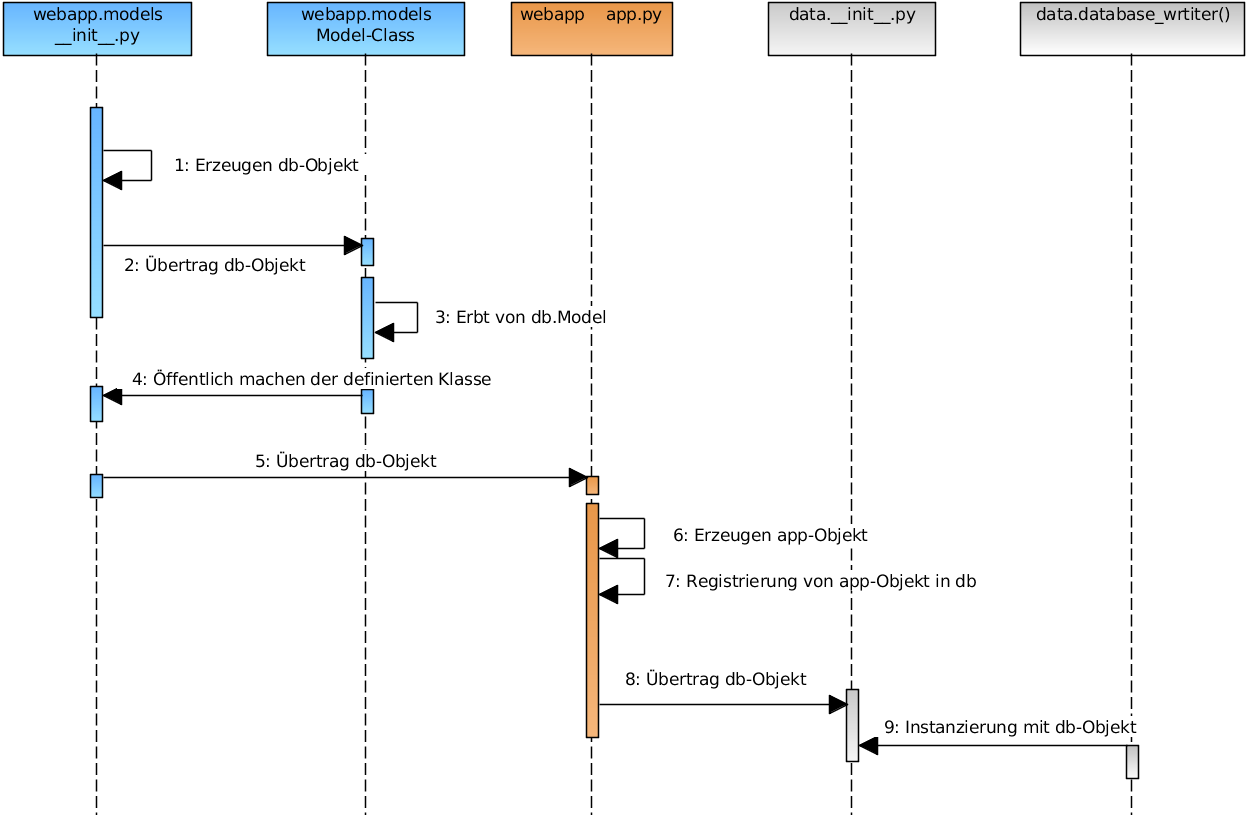
\includegraphics[width=\textwidth]{pix/seq_db.png}
 % seq_db.png: 1310x617 px, 96dpi, 34.66x16.32 cm, bb=0 0 982 463
 \label{fig:sequenzSQLALCHEMY}
 \caption{Sequenzdiagramm der Einbindung von SQLAlchemy}
\end{figure}


\begin{enumerate}
 \item
        In der Datei \texttt{webapp.models.\_\_init\_\_.py} muss sichergestellt werden, dass die SQLAlchemy-Instanz noch vor der Initiierung der Modell-Klassen erzeugt wurde.
 \item
        Nun kann das \texttt{db}-Objekt in die Modellklassen übertragen werden. Dafür importieren diese \texttt{db} in ihren Scope.
 \item
        Die Modell-Klassen werden in \texttt{db} registriert. Dafür erben diese von der Metaklasse \texttt{db.Model}. Siehe auch Listings \ref{lst:models_argofloat} und \ref{lst:models_measurement}.

        \pythonexternal[%
    caption={\texttt{webapp.models.\_\_init\_\_.py}},%
    label={lst:initpy_models}]{/home/sebsch/Dokumente/Uni-Workdir/Bachelorarbeit/BA_argo_proto/webapp/models/__init__.py}


 \item
        Die Modell-Klassen dürfen erst nach der Instantiierung von \texttt{db} über den Scope des Submodules heraus bekannt gemacht werden, um sicherzustellen, dass dieses bereits existiert. Die Implementierung des Ablaufs ist in Listing \ref{lst:initpy_models} ersichtlich.

 \item  \label{enum:seqdbwebapp1}
        Die Instanz \texttt{db} kann nun mit den in ihr registrierten Modell-Klassen  aus dem Submodul in die Datei \texttt{webapp.\_\_init\_\_.py} importiert werden.

\item
        Hier wird nun das globale Objekt der Flask-Instanz (\texttt{app}) erstellt und konfiguriert.

\item   \label {enum:seqdbwebapp3}
        Anschließend wird \texttt{app} in \texttt{db} registriert. Die Schritte \ref{enum:seqdbwebapp1} bis \ref{enum:seqdbwebapp3} können über das Listing \ref{lst:init_webapp} nachvollzogen werden.

\item   Die Instanz \texttt{db} aus dem Scope
        \texttt{webapp.db} ist nun fertig konfiguriert und kann für das Lesen und Schreiben in die Datenbank verwendet werden.
\end{enumerate}


\pagebreak
\subsubsection{Controller}

\pythonexternal[%
    caption={ \texttt{webapp.\_\_init\_\_.py}},%
    label={lst:init_webapp}]{/home/sebsch/Dokumente/Uni-Workdir/Bachelorarbeit/BA_argo_proto/webapp/__init__.py}

% 1. Vorstellung Flask -- warum gewählt; Vor- und Nachteile

Über die globale Instanz des \gls{Controller}s (\texttt{app}) kann auf Daten zugegriffen und die Konfiguration vorgenommen werden. In Listing \ref{lst:init_webapp} ist die Initialisierung des \gls{Controller}s zu sehen.
% 2. Trennung von API und APP in verscheidene Blueprints

Über Blueprints wird die in Kapitel \ref{sec:entwurfRoutes} ausgearbeitete logische Trennung zwischen \texttt{app} und \texttt{api} realisiert. Die hier definierten Module umfassen auch die in diesem Kontext benötigten Hilfsprogramme. Die hier implementierte Modulstruktur von \texttt{argo\_api} und \texttt{argo\_app} ist im Folgenden ersichtlich.

\begin{description}
 \item [argo\_api] $ $

    \begin{description}
     \item [query\_factory]
        Alle lesenden Zugriffe zur Datenbank werden über eine QueryFactory zentral zusammengefasst. Die hier ausgearbeitete Implementierung ist in Kapitel \ref{sec:implementierungORM} ausführlich beschrieben.

     \item [json\_builder]
        Durch diese Programmabschnitte werden die Daten in Listen und Dictionaries überführt. Die Variablen und Datenstrukturen werden dabei so angelegt, dass diese direkt als JSON bzw geoJSON ausgeliefert werden können.
    \end{description}

    Dieses \gls{Controller}-Blueprint fordert die Daten über die \texttt{query\_factory} an und bringt sie über den \texttt{json\_builder} in das vorgesehene Format.  Die Umwandlung in JSON und die Erstellung des Requests erfolgt über \texttt{flask.jsonify}.
\pagebreak
 \item [argo\_app] $ $

    \begin{description}
     \item [generate\_graph] Dieser Programmteil erzeugt einen Plot über die Bibliothek \texttt{matplotlib}. Eine nähere Beschreibung der Erstellung findet sich in Kapitel \ref{sec:ImplementierungPLOTS}.
    \end{description}

    In diesem Blueprint werden Templates zu HTML-Dateien zusammengesetzt. Dafür benötigt dieser Programmteil Zugriff auf die Verzeichnisse für die jeweiligen Templates und statischen Dateien. Diese Daten werden über \texttt{flask.render\_template} zusammengesetzt und ausgeliefert.
\end{description}

Die so erstellten Blueprints werden im zentralen \gls{Controller} (\texttt{app}) über das Schlüsselwort \texttt{app.register\_blueprint} registriert und zusammengefasst.
Als zentrale Steuerungseinheit für den gesamten Programmablauf dient die Datei \texttt{manage.py}. Die Parameter dieser Datei werden im Folgenden kurz beschrieben:

\begin{description}

 \item [runserver] Durch diesen Parameter wird der Server der Applikation gestartet.


 \item [rebuild\_db] Dies stößt den Prozess der Datenaggregation an.  Streng genommen ist dies nicht Teil des \gls{Controller}s. Aus Gründen der Einfachheit wurde dieser Programmablauf aber in die Steuerungseinheit integriert.

 \item [shell] Durch diesen Parameter wird eine IPython-Shell gestartet. In diesem repl ist die Webapplikation mit all ihren Umgebungsvariablen initiiert. Diese Shell dient für das Debugging der Applikation.

 \item [list\_routes] Dieser Parameter listet alle Routen, die durch den Controller definiert sind auf der Kommandozeile auf.
\end{description}


\subsubsection{Templates}
% jinja2

Für das Erstellen der HTML-Dateien wurde die Template-Engine Jinja2 verwendet. Diese ist gut in Flask integriert. Jinja2 erlaubt das Modularisieren von HTML-Dateien, den Zugriff auf Variablen und übergebenen Daten sowie die Abarbeitung einfacher Strukturen und Wahrheitswerte.

% Modulare Struktur  ..?

Die Templatestruktur wurde in dieser Applikation stark modularisiert.  In Listing \ref{lst:templateMAP} ist der Einstieg in die Modulstruktur zu sehen und im Folgenden beschrieben.
\pythonexternal[%
    caption={ \texttt{webapp.templates.map.html}},%
    label={lst:templateMAP}]{/home/sebsch/Dokumente/Uni-Workdir/Bachelorarbeit/BA_argo_proto/webapp/templates/map.html}

Die Datei \texttt{\_base.html} ist für die Darstellung der Webseite verantwortlich. Diese wurde über Twitter Bootstrap realisiert. Als Vorlage diente dabei ein bereits ausgearbeitetes  \texttt{2-Column Layout} aus \cite{Ng2014}. Der Beispielcode wurde an die Anforderung der Applikation angepasst. Der Code wurde dabei in die logischen Bestandteile zerlegt und in die modulare Struktur der Webseite überführt. Der Code ist unter einer MIT Lizenz veröffentlicht. Damit kann der Code unter Nennung der Lizenz verwendet werden. Deswegen wurde ein Tag in das HTML Element eingesetzt, um Autor und Lizenz zu nennen.

\subsubsection{Kartendarstellung}

 OpenLayers ist eine Programmbibliothek um interaktive Geoapplikationen zu entwickeln. Das \gls{Framework} ist in Javascript entwickelt und nimmt alle benötigten Berechnungen auf Clientseite vor. Die Bibliothek erlaubt es, Kartenmaterial aus verschiedensten Quellen zu rendern. Dabei können Kachel- oder auch Vektorbasierte Materialien eingebunden werden.
Die Elemente der Karte setzen sich, wie in Listing \ref{lst:olMap} zu sehen, zusammen.

\begin{javascript}[label={lst:olMap}, caption={Das ol.Map Element aus der Kartendarstellung}]
 var map = new ol.Map({
    layers: [mapVectorLayer, argoFloatsLayer],
    target: 'map',
    controls: ol.control.defaults({
        attributionOptions: false,
        zoom: false,
    }),
    view: new ol.View({
        center: [0, 0],
        zoom: 3.5,
        minZoom: 3
    })
});
\end{javascript}

Die Darstellung bassiert auf zwei Layern, einer Verktordarstellung der Kontinent- und Landesgrenzen (\texttt{mapVectorLayer}), sowie der Darstellung der ArgoFloats (\texttt{argoFloatsLayer}). Die Darstellung der Steuereinheiten wurde deaktiviert. Als Startposition wurden Längen- und Breitengrad mit jeweils 0 gewählt. Die Zoomstufe ist mit 3 initialisiert und es ist eine maximale Zoomstufe von 3.5 gewählt. Die Werte für die Zoomstufe wurden bei einer Auflösung von 1920x1080 ermittelt und getestet.
Die Karte bettet sich in das HTML-Element map ein und wird mit diesem zur Anzeige gebracht. Steuergesten mit Maus und Tastatur nimmt die Karte an dieser Stelle bereits entgegen.
\\
Der mapVectorLayer wurde aus der GeoJSON-Datei \texttt{countries.geo.json}  erstellt. Die Datei wurde von \cite{sundstrm16} heruntergeladen. Diese steht unter der Lizenz UNLICENSE und kann damit ohne Einschränkungen verwendet werden. Die Darstellung der Argo-Floats wird ebenso über eine GeoJSON realisiert. Diese wird auf dem Webserver über die API bereitgestellt und wird über der URL \texttt{/last\_seen}  (siehe Listing \ref{lst:routesAPI}) angefordert. Die so angeforderte Datenstruktur hat ein spezifisches Format. In Listing \ref{lst:argGeoJson} ist das Format in einem gekürzten Format ersichtlich.

\begin{javascript}[label={lst:argGeoJson}, caption={Gekürzte geoJSON zur Darstellung der Argo-Floats}]
 {
"crs": {
    "properties": {
      "name": "EPSG:4326"
    },
    "type": "name"
  },
  "features": [
    {
      "geometry": {
        "coordinates": [
          -52.02875,
          12.92591
        ],
        "type": "Point"
      },
      "properties": {
        "feature_type": "latest_position",
        "identifier": "1901673",
        "last_seen": "Sun, 10 Feb 2013 00:00:00 GMT"
      },
      "type": "Feature"
    },
    // (feature_2, ..., feature_n)
    ]
}
\end{javascript}

Der Parameter \texttt{crs} (Coordinate Reference System Objects) bestimmt die Art der Kartenprojektion. Durch das property \texttt{EPSG:4326} wurde der GPS-Standard WGS84 - World Geodetic System 1984 eingesetzt. Dies deckt sich auch mit den durch die Messstationen bereitgestellten Geo-Koordinaten. Für die Darstellung werden diese Koordinaten in eine Merkatordarstellung (EPSG:3857) projiziert.
\\
Die Repräsentationen der Messstationen finden sich im Array \texttt{features}. Im Feld \texttt{geometry} werden Position und die Form des Features eingestellt. Über \texttt{properties} werden die zusätzlichen Daten \texttt{feature\_type}, \texttt{identifier} und \texttt{last\_seen} in diesem Format gespeichert.
Openlayers kann ein derartig formatiertes GeoJson selbstständig zur Anzeige bringen. Wie die Datei geladen wird, ist in Listing \ref{lst:argoFloatsLayer} zu sehen.
\pagebreak
\begin{javascript}[label={lst:argoFloatsLayer}, caption={Die Funktion argoFloatsLayer}]
var argoFloatsLayer = new ol.layer.Vector({
    style: FloatStyle,
    source: new ol.source.Vector({
        format: new ol.format.GeoJSON(),
        url: "/last_seen"
    })
});
\end{javascript}
Als Quelle für die Anzeigedaten wird hierbei ein \texttt{ol.source.Vector}-Objekt gewählt. Das Format und die \texttt{url} für die spezifizierte Datenquelle werden als Parameter übergeben.
Damit werden die ArgoFloats auf einer vektorbasierten Karte angezeigt.
\\
Was zu diesem Zeitpunkt noch fehlt, ist die Möglichkeit mit den ArgoFloats zu interagieren. Bei Hovern mit dem Mauszeiger über einer ArgoFloat soll ein Tooltip mit einigen Informationen erscheinen und die Messstation optisch hervorgehoben werden.  Die Hervorhebung wird durch den Befehl \jsinline{map.addInteraction(hoverInteraction)} in der Karte registriert. \texttt{overInteraction} ist eine Instanz von \jsinline{ol.interaction.Select} und erlaubt die Auswahl von Features und des Event-Typs. In diesem Fall werden alle Features des \texttt{argoFloatsLayer} ausgewählt, die unter dem Mauszeiger liegen. Openlayers wählt mit dieser Konfiguration einen Vergrößerungseffekt um das Feature hervorzuheben.

Um den Tooltip zur Anzeige zu bekommen, wurde eine weitere Funktion definiert. In Listing \ref{lst:pointermove} ist die Funktion für das Fangen eines \texttt{pointermove}-Events zu sehen.
\begin{javascript}[label={lst:pointermove}, caption={Das Abfangen eines pointermove-Events}]
map.on('pointermove', function (evt) {
    if (evt.dragging) {
        info.tooltip('hide');
        return;
    }
    displayFeatureInfo(map.getEventPixel(evt.originalEvent));
});
\end{javascript}

Die Funktion wartet auf definierte Eingaben. In diesem Fall wird der Funktionskörper durch das Bewegen des Mauszeigers über der Kartendarstellung ausgelöst. Der Event wird als \texttt{evt} in die innere Funktion überführt. Dort wird überprüft, ob es sich um einen dragging-event handelt. Ist dies der Fall, wird der DIV-Container mit der id \texttt{\#info} (\texttt{info}) ausgewählt und der darin liegende Tooltip über den CSS-Parameter \texttt{hide} versteckt. Diese Einstellung wurde gewählt, um störende Tooltips bei der Navigation mit der Karte zu unterbinden. In jeden anderen Fall wird der Pixel an der Spitze des Mauszeigers extrahiert und der Funktion \texttt{displayFeatureInfo} übergeben.
\\
\texttt{displayFeatureInfo} positioniert das info-Element in der Nähe des Mauszeigers und extrahiert etwaige unter dem Pixel liegende Features. Anschließend werden die Attribute des Features untersucht. Über den Befehl \jsinline{feature.get("feature_type") === 'latest_position'} werden Features aus dem \texttt{last\_seen}-GeoJson identifiziert. Ist die Identifikation positiv, werden weitere Attribute extrahiert und in den Text des Tooltips überführt. Zum Abschluss wird der Tooltip über seine CSS-Attribute zur Anzeige gebracht.

Die Funktion kann auch die Features der Positionshistorie einer Boje über einen Tooltip anzeigen. Da sich die hier darzustellenden Parameter unterscheiden, werden dessen Daten gesondert abgefragt.
\\

Die Interaktion über einen Klick passiert analog. In Listing \ref{lst:clickEvent} ist die hier verwendete Implementierung der Klick-Event-Abfrage gezeigt.
\begin{javascript}[label={lst:clickEvent}, caption={Das Abfangen eines Klick-Events}]
map.on('click', function (evt) {
    displayArgoData(map.getEventPixel(evt.originalEvent));
    displayPositions(map.getEventPixel(evt.originalEvent))
});
\end{javascript}

Auch an dieser Stelle wird die \texttt{map.on}-Funktion der Karte verwendet, um den Event abzufangen. Ist dieser vom Typ \jsinline{'click'}, so werden die darauf folgenden Funktionen mit dem Pixel an der Position des Mauszeigers aufgerufen. Im Folgenden wird der Programmablauf der hier aufgerufenen Funktionen erläutert:

\begin{description}
 \item [\texttt{displayArgoData}]
    Diese Funktion ist für die Darstellung der Messdaten, sowie des Informationstextes der ausgewählten ArgoFloat verantwortlich. Aus diesem Grund besteht sie aus zwei Unterfunktionen.
    \begin{description}
    \item [\texttt{display\_chart}]
        Diese Funktion stellt den Funktionsplot der Messwerte der ausgewählten ArgoFloat dar. Dafür wird am Anfang der div-Container mit der ID \texttt{\#chart-picture} ausgewählt. In diesem Container wird später das Bild platziert. Um bereits bestehende Bilder zu löschen, werden alle HTML-Elemente innerhalb des Containers erstellt. Anschließend wird das Bild der Messdaten über die Webroute /chart/[identifier]  (siehe Listing \ref{lst:routesAPI}) angefordert. Das Bild wird anschließend auf die Breite des Containers gebracht und der Bootstrap-Klasse \texttt{img-responsive} hinzugefügt. Damit wird das Bild formatiert über die Sidebar dargestellt.
    \item [\texttt{display\_info}]
        Diese Funktion stellt einen Info-Block zu den Metadaten der ArgoFloat dar. Analog zum oberen Prozess werden hier Container aus dem DOM-Tree selektiert und das sich darin befindliche  HTML manipuliert. Die Daten wurden hier als HTML-Objekte über einen Ajax-Befehl angefordert und direkt in den umliegenden Container injiziert.
    \end{description}

    Die oben genannten Funktionen werden aufgerufen, wenn es sich bei dem angeklickten Element um ein Feature vom Typ \texttt{Point} handelt. Der Bereich des Graphen wird an dieser Stelle sichtbar gemacht und der Info-Bereich eingeklappt. Die Sichtbarkeit der Sidebar wird ebenso an dieser Stelle eingestellt.

 \item [\texttt{displayPositions}]
    Diese Funktion stellt eine Positionshistorie einer spezifischen Messstation dar. Dafür wird ein GeoJSON über die url \texttt{/positions/[identifier]} angefordert. Das Sichtbar-Machen, der hier kodierten Daten geschieht analog zu der Darstellung aller Argo-Floats. Das GeoJson trägt zusätzlich noch ein \texttt{LineString}-Element, um den zeitlichen Verlauf der Positionen zu verdeutlichen.
\end{description}





\subsubsection{Zeichnen der Graphen} \label{sec:ImplementierungPLOTS}

% 1- verwendete Software, Vor und Nachteile, warum gewählt

Für die Darstellung der Messwerte wurde sich in dieser Applikation für die Python-Bibliothek \texttt{matplotlib} entschieden.  Diese Plotting-Engine ist in der Entwicklung von wissenschaftlichen Applikationen in Python sehr verbreitet.
Als Renderer wurde ein AGG-Renderer eingesetzt. Dieser erlaubt das Vorhalten der Bilddaten im Arbeitsspeicher, sowie deren Überführung in ein Canvas-Element.

In Listing \ref{lst:deliver_chart} ist die Funktion des \gls{Controller}s zu sehen, über die das Bild bereit gestellt wird.

\begin{python}[label={lst:deliver_chart}, caption={Ausliefern eines Funktionsplots Flask}]
@argo_app.route("/chart/<identifier>")
def deliver_chart(identifier):
    url = url_for('argo_api.get_argo_float', identifier=identifier, _external=True)
    data = requests.get(url).json()

    fig = create_plot(data)
    canvas = FigureCanvas(fig)
    png_output = BytesIO()
    canvas.print_png(png_output)
    response = make_response(png_output.getvalue())
    response.headers['Content-Type'] = 'image/png'

    return response
\end{python}

Die Funktion wird im Blueprint \texttt{argo\_app} der Flask-Applikation mit der Route registriert. Als Parameter \texttt{identifier}  wird die eindeutige Identifikationsnummer der Messstation erwartet. Die zum Erstellen des Graphen benötigten Daten werden aus der API angefordert. Dafür wird die URL der Datenschnittstelle der Methode \texttt{get\_argo\_float} in der API ermittelt. Anschließend wird unter Zuhilfenahme der Python-Bibliothek \texttt{requests} der Datensatz über einen GET-Request angefordert. Die Methode \texttt{.json()} überführt die Daten von Json in eine Python-Datenstruktur.

\begin{description}
 \item [\texttt{create\_plot}]
    Diese Funktion ist für die Erstellung des Funktionsplots zuständig. Als Theme wurde sich hier für \texttt{'seaborn-whitegrid'} entschieden. Eine der damit vorgegebenen Grundeinstellungen wurden durch das Ändern der \texttt{rcParams} noch weiter angepasst.\\
    Für die Darstellung jeder der drei Funktionsplots wurden ein Achsen-Objekt erstellt. Diese Achsen werden über ein Gridspec untereinander angeordnet.

    Die Datensätze werden über die Y-Achse aufgetragen, wärend die X-Achse die Zeitstempel aufzeigt. Enthält ein Datensatz Werte keiner numerischen Zuordnung (\texttt{nan}), so wird davon ausgegangen, dass dieser Datensatz nicht vorhanden ist und diese Achse nicht gezeichnet. Überschreitet ein Datensatz den ihm zugeschriebenen Wertebereich, so wird der Wertebereich der Y-Achse fest eingestellt. Die hierfür benötigten Daten werden über die zentrale Flask-Instanz aus der Konfiguration angefordert.

    Um den Platz besser nutzen zu können, wird die Beschriftung der Y-Achse nur auf dem untersten Graphen aufgetragen. Dieser enthält die Werte für den Druck des umliegenden Wassers. Dieser Messwert sollte in jeder Boje enthalten sein, es ist also nicht davon auszugehen, dass dieser Wert nicht gezeichnet wird.

    Die Achsen werden über das Gridspec in einer \texttt{Figure} zusammengefasst und damit aus dem Funktionskontext zurückgegeben.
\end{description}

Der so erstellte Funktionsgraph wird als Canvas-Element in einen response eingebunden und über diesen ausgeliefert.






% 2- Anfodern der Daten aus der API
% 3- Ablauf -- halten der Figure im RAM AGG-Renderer
% 4- Aufbau der Plotfunktion
% 5- Bereistellung des Bildes über response

%END

\section{Testen}

\subsection{Funktionstest}

\subsubsection{Webapplikation}

Um die Webapplikation zu testen, wurde ein Funktionstest durchgeführt. Dieser umfasst die in Kapitel \ref{sec:funkAnforderungenAnwender} festgesetzten Anforderungen und ist im Folgenden bebildert beschrieben.\newline



\begin{wrapfigure}[9]{l}{0.4\textwidth}
 \centering
 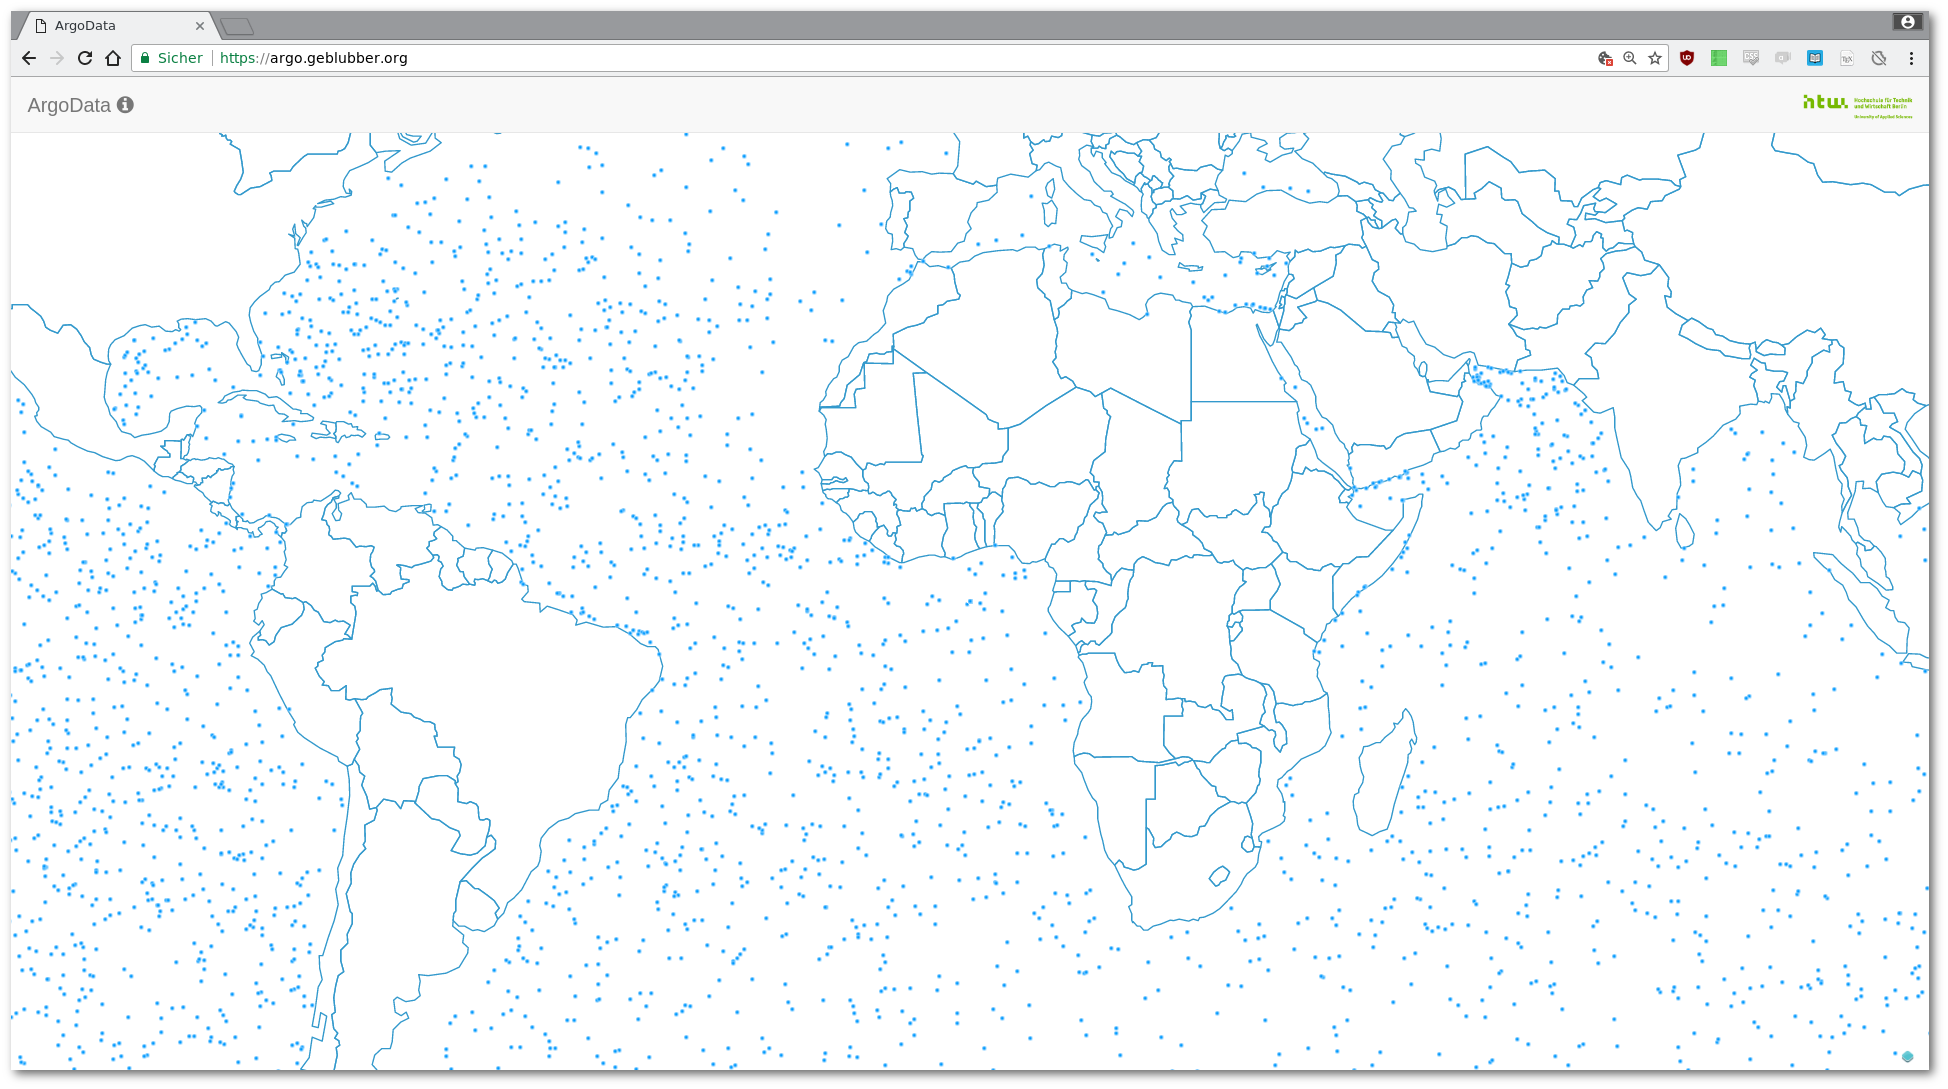
\includegraphics[width=0.39\textwidth]{pix/ftest/001.png}

 \caption{\textbf{Funktionstest I} Der Aufruf der Webapplikation}
 \label{fig:ftest001}
\end{wrapfigure}


Wie in Abbildung \ref{fig:ftest001} zu erkennen ist, werden die Grenzen der Ozeane und Kontinente über eine Weltkarte dargestellt, wenn die Webpräsenz der Applikation unter der für ArgoData registrierten Url aufgerufen wird. Die Karte ist über eine Vektorrepräsentation dargestellt, Landmarker wie Straßen und Städte sind darauf nicht zu erkennen. Die letzte Position der Messstationen ist über die jeweilige Position auf der Karte ersichtlich.
\newline\newline\newline


\begin{wrapfigure}[10]{l}{0.4\textwidth}
 \centering
 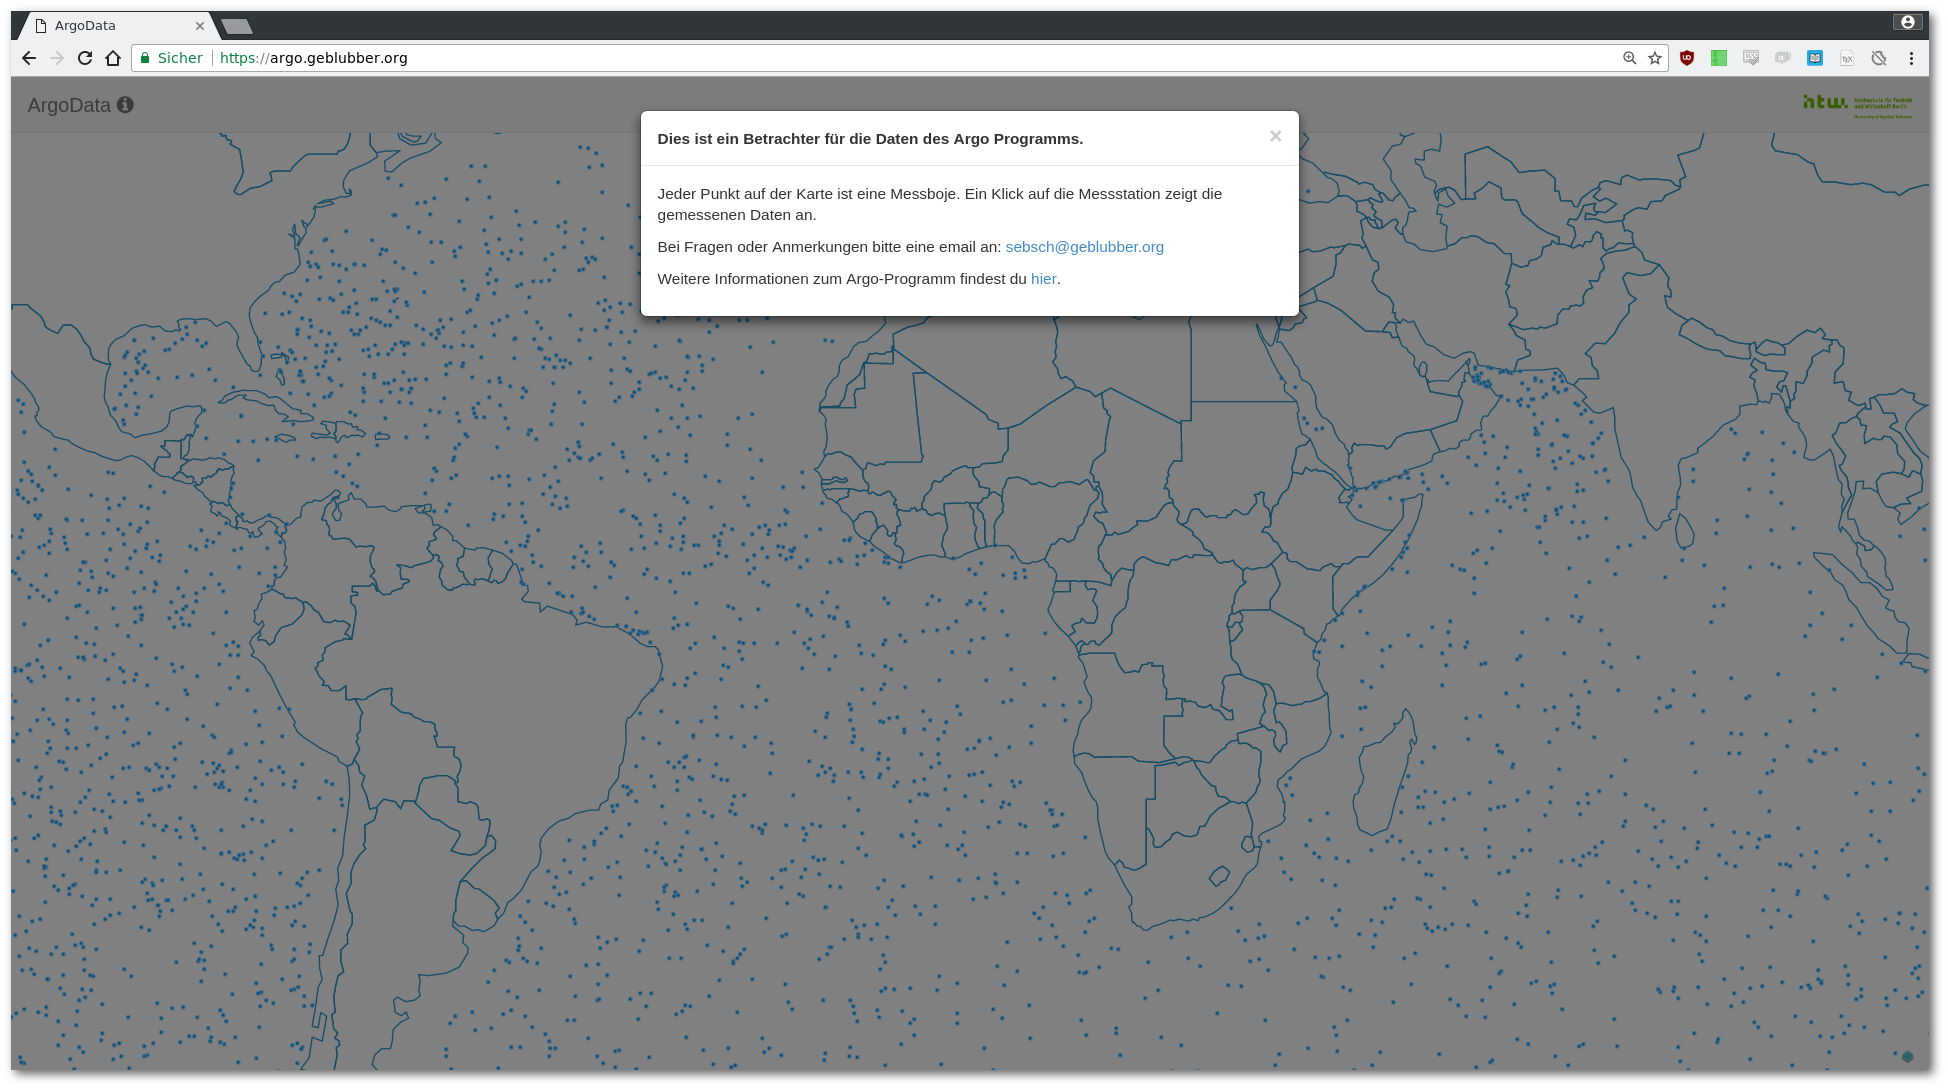
\includegraphics[width=0.39\textwidth]{pix/ftest/001b.png}
 \caption{\textbf{Funktionstest II} Die Anzeige der Hilfe}
 \label{fig:ftest001b}
\end{wrapfigure}

Durch Anklicken des Infobuttons erhält der Benutzer über ein Modal eine Kurzhilfe angezeigt. Diese erklärt die grundlegende Funktion der Webseite, stellt Kontaktdaten bereit und stellt über einen Web\-link eine Verbindung zum Argo-Programm her. In Abbildung \ref{fig:ftest001b} ist die Webseite mit aktiviertem Modal zu sehen.
\newline\newline\newline\newline \newpage


\begin{wrapfigure}[10]{l}{0.4\textwidth}
 \centering
 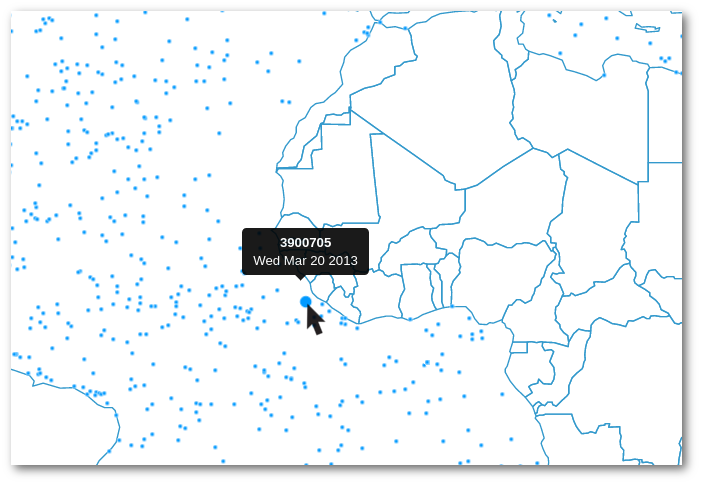
\includegraphics[width=0.39\textwidth]{pix/ftest/002.png}

 \caption{\textbf{Funktionstest III} Mousehover über Messstation}
 \label{fig:ftest002}
\end{wrapfigure}

Wird der Mauszeiger über die Repräsentation einer Messstation geführt, so erscheinen grundlegende Daten der Argo-Boje. Dies umfasst den eindeutigen Identifier sowie das Datum des letzten Messvorgangs. Zu erkennen in Abbildung \ref{fig:ftest002}.
\newline\newline\newline\newline\newline


\begin{wrapfigure}[10]{l}{0.4\textwidth}
 \centering
 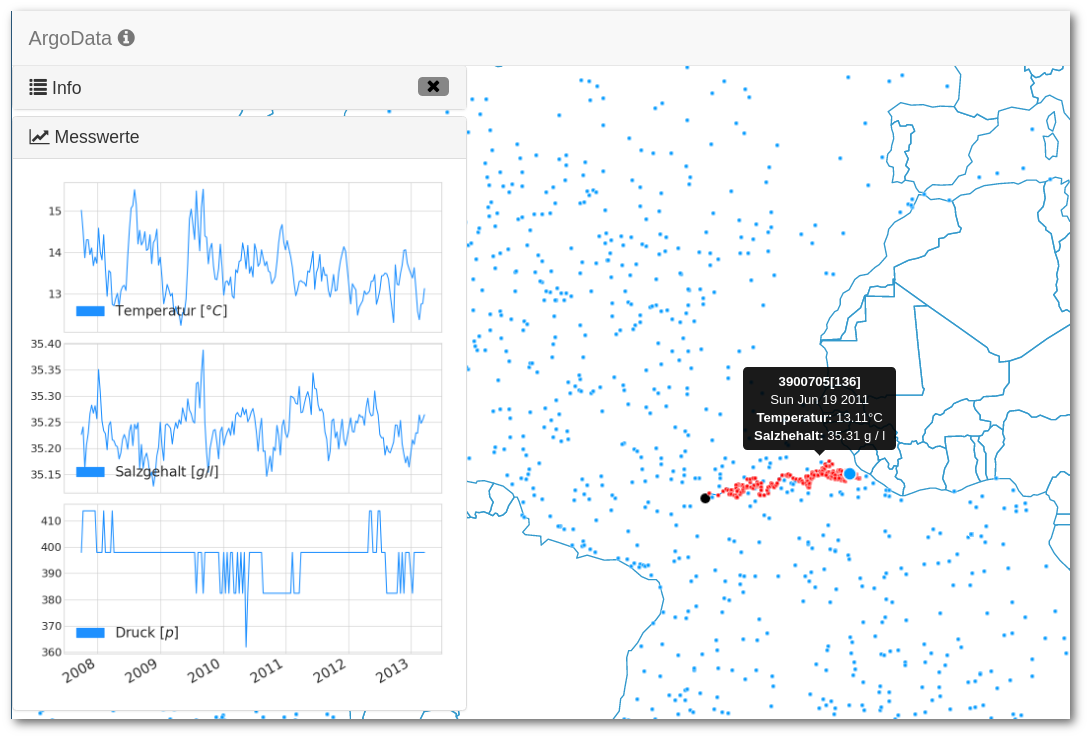
\includegraphics[width=0.39\textwidth]{pix/ftest/003.png}

 \caption{\textbf{Funktionstest IV} Werte werden angezeigt}
 \label{fig:ftest003}
\end{wrapfigure}

Durch einen Mausklick auf die Kartendarstellung der Argo-Boje werden weiterführende Daten angefordert. Wie in Abbildung \ref{fig:ftest003} zu sehen ist, werden  Messwerte  über Funktionsplots an der linken Seite der Webseite dargestellt. Dabei sind über die X-Achse der zeitliche Verlauf und über die Y-Achse der jeweilige Messwert kodiert. Die gemessenen Werte umfassen dabei Temperatur, Salzgehalt sowie Druck.  Der Ort der Messwerterhebung wird durch einen Punkt auf der Karte repräsentiert. Wird der Mauszeiger über diese Repräsentation geführt, werden neben dem Datum der Messung auch die gemessenen Werte dargestellt.

\newpage

\begin{wrapfigure}[10]{l}{0.4\textwidth}
 \centering
 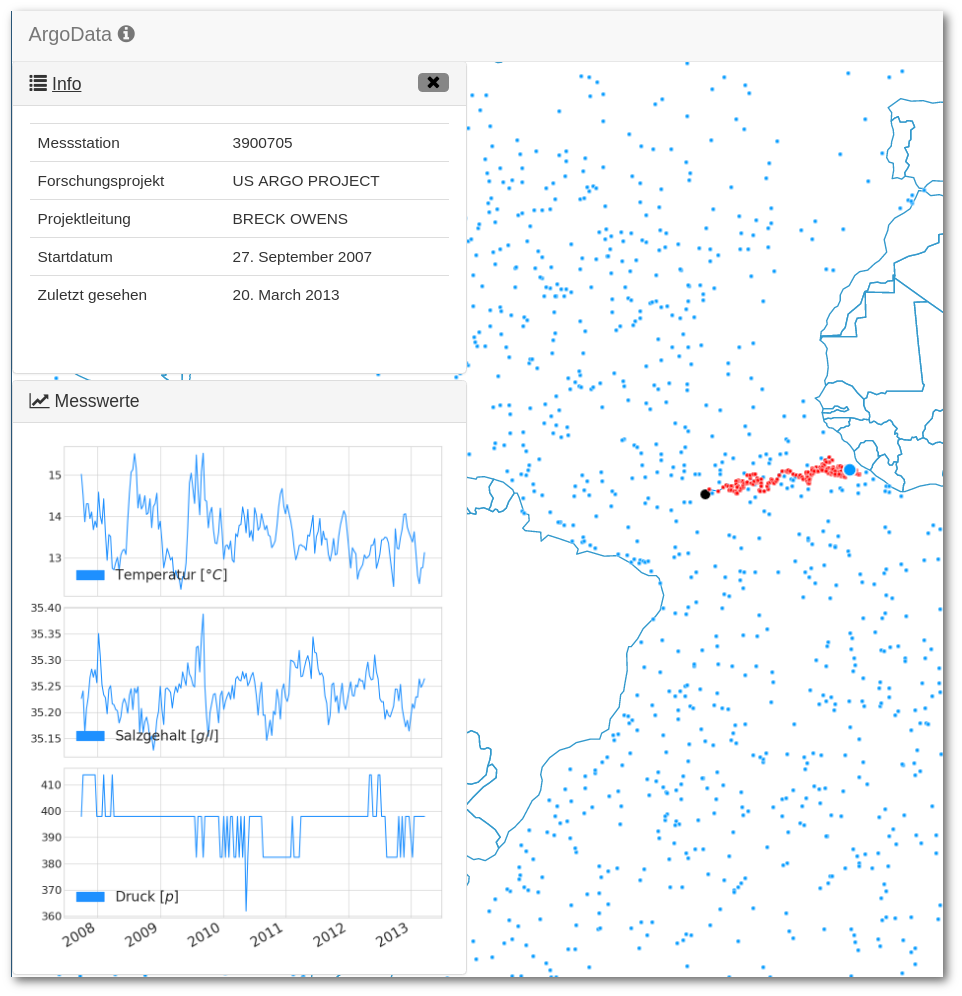
\includegraphics[width=0.35\textwidth]{pix/ftest/003b.png}

 \caption{\textbf{Funktionstest V} Metainformationen werden angezeigt}
 \label{fig:ftest003b}
\end{wrapfigure}

Wird der Reiter "`Info"' angeklickt, so werden weitere Informationen zur Messstation sichtbar. Wie in Abbildung \ref{fig:ftest003b} zu sehen ist,  Umfassen diese den Identifier der Messstation, das verantwortliche Forschungsprojekt, den Besitzer der Boje sowie das Startdatum und das Datum der letzten Messung.
\newline\newline\newline\newline
\newline\newline\newline


\begin{wrapfigure}[10]{l}{0.4\textwidth}
 \centering
 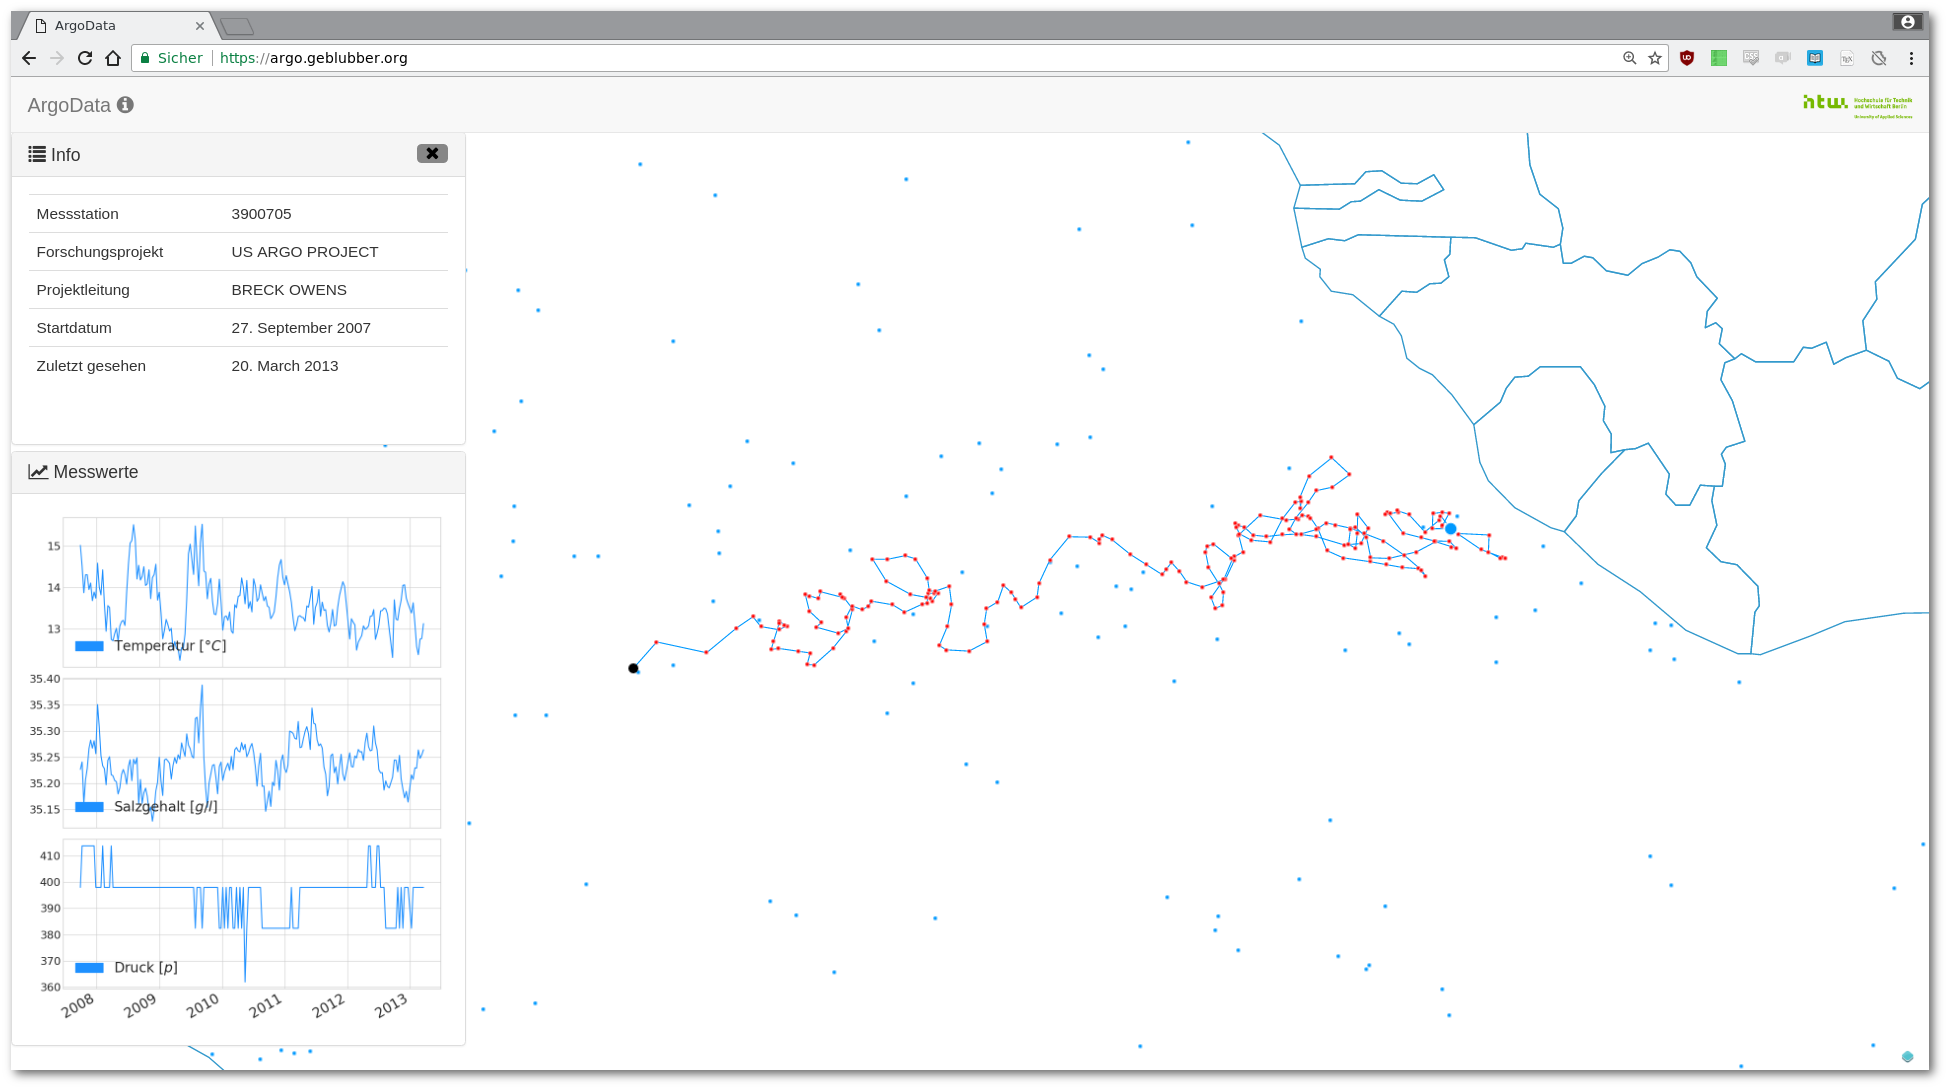
\includegraphics[width=0.35\textwidth]{pix/ftest/004.png}

 \caption{\textbf{Funktionstest VI} Der Pfad der Messstatioon kann zurückverfolgt werden}
 \label{fig:ftest004}
\end{wrapfigure}

Wie in Abbildung \ref{fig:ftest004} zu erkennen ist, wird der zwischen zwei Messpunkten der zurückgelegte Weg über eine Linie dargestellt. Somit kann der Weg, den eine Messstation zurückgelegt hat um die Daten zu erheben, klar nachvollzogen werden.
\newline\newline\newline\newline
\newline\newline\newline


\begin{wrapfigure}[10]{l}{0.4\textwidth}
 \centering
 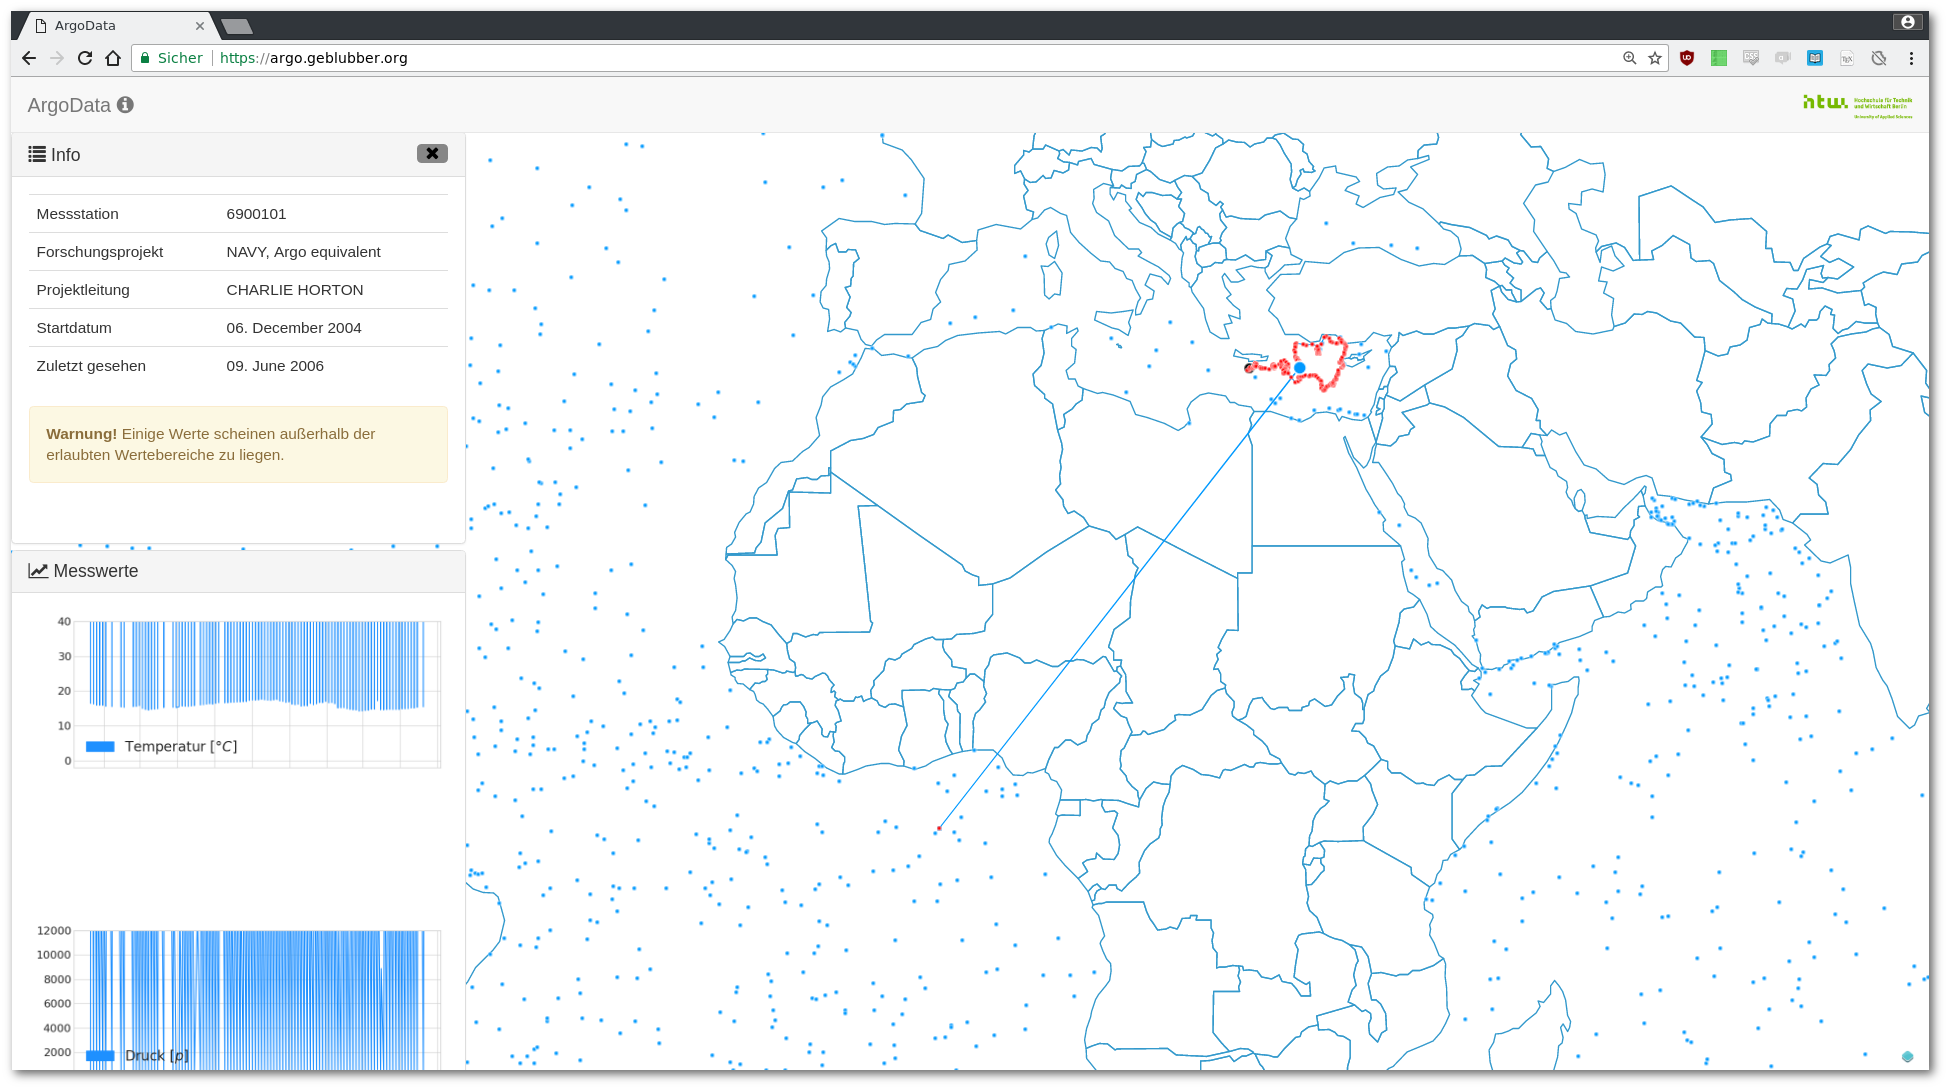
\includegraphics[width=0.35\textwidth]{pix/ftest/00fail.png}

 \caption{\textbf{Funktionstest VI} Fehlerhafte Daten werden markiert}
 \label{fig:ftest00fail}
\end{wrapfigure}

In Abbildung \ref{fig:ftest00fail} ist ersichtlich, dass fehlerhafte Daten durch eine Warnung hervorgehoben werden. Diese informiert die Benutzenden, dass die Daten, die gerade angezeigt werden, zum Teil die Wertebereiche überschritten haben. Die Achsen der Funktionsplots werden auf die Wertebereiche beschränkt und Plots von mit \texttt{nan} kodierten Messwerten nicht dargestellt.
\newline
\newline



\subsubsection{Aggregation der Daten}

In Listing \ref{lst:renewdatash} ist der Prozess der Datenerneuerung zu sehen. Dieser Umfasst die in Kapitel \ref{sec:funkAnforderungenAdmin} festgelegten Anforderungen. Der Ablauf ist im Folgenden beschrieben.

\begin{python}[%
        label={lst:renewdatash},%
        caption={Erneuerung des Datensatzes}]
 -> # bash /root/argo_proto/renew_data.sh
(!) Starting renew process at Tue Mar  6 12:41:24 CET 2018.
 >> Downloading new data...
        done.
Datafolder: /root/aoml/
||||||||||||||||||||||||||||||||||| 6711/6711 [2:02:33<00:00,  1.10s/it]
 >> Dumping tmpdb to /tmp/argo_db.sql ...
        done. [164601410 Mar  6 14:44 /tmp/argo_db.sql]
 >> Renew production database ...
        done.
 >> Renew Argos cache...
        done.

Process finished.
This took  7381 seconds.
We had a downtime of 11 seconds.
So long and thanks for all the fish. Bye.
\end{python}

\begin{description}
 \item [Daten herunterladen]
    Die Daten des Argo-Programms werden heruntergeladen. Es handelt sich um die Livedaten nach der Qualitätskontrolle aus der Quelle \texttt{aoml}. Für das herunterladen wird rsync verwendet. In der Quelle nicht mehr vorhandene Daten werden gelöscht.


 \item [Daten aggregieren]
    Der Aggregationsteil der hier entwickelten Software wird verwendet, die soeben erneuerten Daten in die Datenbank zu überführen. Um Ausfallzeiten der Webapplikation möglichst gering zu halten, werden die Daten zunächst in eine temporäre Datenbank geschrieben. Über einen Ladebalken wird der derzeitige Stand dieses Prozesses sichtbar. Es ist außerdem ersichtlich, dass die Daten von 6711 Messstationen in 2 Stunden, 2 Minuten und 30 Sekunden in die Datenbank überführt wurden.

 \item [Erstellen eines Datenbankdumps]
    Um die Daten in die Produktionsdatenbank zu überführen, werden die Tabellen der temporären Datenbank gedumpt. Es ist ersichtlich, dass der Dump eine Größe von  ca. 20 Megabyte umfasst.

 \item [Einspielen des Datenbankdumps]
    Über die Funktionalitäten des Postgresql-Clients \newline\texttt{psql} werden die Daten in die Produktionsdatenbank überführt. Dieser Prozess erfordert eine Ausfallzeit der Webapplikation von 11 Sekunden.

 \item [Erneuern des Caches zur Anzeige der Argo-Floats]
    Um die Daten in der Anzeige zu erneuern, wird der Cache neu geschrieben. Für diesen Zweck wird ein GET-Request an die hierfür festgelegte URL gesendet. Die Webapplikation erneuert daraufhin den Cache. Damit stehen der Webapplikation die erneuerten  Daten zur Verfügung.
\end{description}



\newpage
\subsection{Usability-Umfrage}

\subsubsection{Testaufbau}

Um die Usability der Webapplikation zu testen, wurde eine Umfrage durchgeführt. Als Grundlage diente der System Usability Scale (SUS).
Für diese Umfrage waren insgesamt 10 Fragen innerhalb einer Scala von 0 (gar nicht) bis 5 (sehr)  zu bewerten. (vgl. \cite{Quantita52:online})

An der Umfrage nahmen insgesamt 12 Personen teil. Diese setzen sich aus Bekannten- und Kollegenkreis zusammen. Die Daten wurden anonym erhoben, ein Rückschluss auf die Personen ist damit nicht mehr möglich.

In Abbildung \ref{fig:surveyAuswertung}
ist eine grafische Zusammenfassung der Ergebnisse zu sehen. In dieser findet sich zu jeder Frage ein Balkendiagram der akkumulierten Häufigkeit, kombiniert mit einem Box-Whisker-Plot. Dieser setzt sich aus folgenden Elementen zusammen:

\begin{description}
 \item [Box]
    Dies markiert den Bereich in welchem sich 50\% der Daten finden. Der Median wird durch eine vertikale Linie gezeigt. Die hier vorliegende Darstellung ist um den Mittelwert (mean) erweitert. Die schmale Linie stellt das arithmetische Mittel und die fett gedruckte den Median dar.
 \item [Whisker (Antennen)]
    Dieser Bereich stellt die äußeren Quantile dar. In der hier verwendeten Grundeinstellung 1.5 wird die von John W. Turkey verwendete Einstellung von maximal dem 1.5-fachen des Interquartilabstandes für den Whiskerbereich verwendet.
\end{description}


\subsubsection{Testauswertung}

Im Folgenden findet sich eine detaillierte Auswertung der hier erhobenen Daten:


\paragraph{\texttt{Statement 1:} "`Ich kann mir gut vorstellen, ArgoData regelmäßig zu nutzen."'}
    Diese Frage zielt auf die Wiederbesuchsbereitschaft ab. Die Antworten weisen eine breite Streuung auf. Die am häufigsten gegebene Antwort liegt bei 4 (4 von 12 Personen). Der Median liegt bei 3, das arithmetische Mittel befindet sich bei $2.67$. Die Box umfasst die Antworten 2 bis 4. Der Whisker schließt Antwort 1 mit ein.

 \paragraph{\texttt{Statement 2:} "`Ich empfinde ArgoData als unnötig komplex."'}
    In dieser Frage, bildet sich die Reduktion der Komplexität ab.
    Die am häufigsten gegebene Antwort liegt bei 1 (7 von 12 Personen).  Der Median liegt bei 1, das arithmetische Mittel bei $1.67$. Die Box umfasst die Antworten 1 bis 2. Der Whisker schließt Antwort 3 mit ein.

  \paragraph{\texttt{Statement 3:} "`Ich empfinde ArgoData als einfach zu nutzen."'}
    Durch diese Frage wird die Einfachheit der Darstellung und die Reduktion der Benutzungskomplexität abgebildet. Die am häufigsten gegebene Antwort liegt bei 5 (6 von 12 Personen). Der Median liegt bei $4.5$, das arithmetische Mittel bei $4.25$   Die Box umfasst Antworten 4 und 5. Der Whisker schließt Antwort 3 mit ein.

\paragraph{\texttt{Statement 4:} "`Ich denke, dass ich Hilfestellung bei der Benutzung brauchen würde um ArgoData zu benutzen."'}
    Diese Frage ermittelt ob genügend Hilfestellung zur Verfügung gestellt wurde.  Die am häufigsten gegebene Antworten liegen bei 1 und 3 (4 von 12 Personen).  Der Median liegt bei 2.5, das arithmetische Mittel liegt bei $2.33$. Die Box umfasst Antworten 1 bis 3, der Whisker schließt Antwort 4 mit ein.

\paragraph{\texttt{Statement 5:} "`Ich finde, dass die Funktionen (Karte, Steuerung, Anzeige von Daten) gut integriert sind."'}
    Diese Frage ermittelt die Integration der Steuerungselemente. 
    Die am häufigsten gegebene Antwort liegt bei 4 (6 von 12 Personen). Der Median liegt bei 4, das arithmetische Mittel bei $4.33$. Die Box umfasst  die Antworten 4 und 5. Der Whisker schließt Antwort 3 mit ein.

\paragraph{\texttt{Statement 6:} "`Ich finde, dass es in ArgoData zu viele Inkonsistenzen gibt."'}
    Diese Frage zielt auf die Integration der Komponenten als Gesamtkonzept ab. Die am häufigsten gegebene Antwort liegt bei Antwort 2 (5 von 12 Personen). Der Median liegt bei 2, das arithmetische Mittel bei $2.08$. Die Box umfasst Antworten 2 und 3. Der Whisker schließt Antwort 1 mit ein.

\paragraph{\texttt{Statement 7:} "`Ich kann mir vorstellen, dass die meisten Leute ArgoData schnell zu beherrschen lernen."'}
    Diese Frage versucht über eine extrene Perspektive die Lernkurve bei der Benutzung abzufragen.Die am häufigsten gegebene Antwort liegt bei 5 (6 von 12 Personen). Der Median liegt bei 4.5, das arithmetische Mittel bei $4.42$. Die Box umfasst die Antworten 4 und 5. Der Whisker schließt Antwort 3 mit ein.

\paragraph{\texttt{Statement 8:} "`Ich empfinde die Bedienung als sehr umständlich."'}
    Diese Frage versucht das Erleben des Bedienungskonzeptes zu erfragen. Die am häufigsten gegebene Antwort liegt bei 2 (7 von 12 Personen). Der Median liegt bei 2, das arithmetische Mittel bei $1.75$ Die Box umfasst die Antworten 1 und 2. Der Whisker schließt Antwort 3 mit ein.

\paragraph{\texttt{Statement 9:} "`Ich musste eine Menge Dinge lernen, bevor ich mit ArgoData arbeiten konnte."'}
    Diese Frage ermittelt die Lernkurve die zur Benutzung notwendig ist. Die am häufigsten gegebene Antwort ist die 1 (9 von 12 Personen). Der Median liegt bei Antwort 1, das arithmetische Mittel bei $1.5$. Die Box umfasst Antwort 1, der Whisker schließt keine weiteren Antworten mit ein, diese sind damit als Ausreißer zu betrachten.

\subsubsection{Interpretation der Ergebnisse}
Die Antworten sind durchwegs als positiv zu betrachten. Die Fragen zur Komplexität lassen erkennen, dass es gelungen ist, die wissenschaftlichen Daten ohne Vorkenntnisse verstehbar darzustellen. Die Bedienungsmuster wurden angenommen und als konsistent und wenig umständlich beschrieben. Die Frage zur Wiederbesuchsbereitschaft weist eine starke Streuung auf. Da es sich um eine Seite mit einem Bildungsangebot handelt, ist dies erklärbar.
Ein klarer Verbesserungswunsch lässt sich aus der Frage zu den angebotenen Hilfestellungen ableiten. Hier gilt es  zu überlegen, ob und in welcher Form den benutzenden Personen zur Hand gegangen werden kann.



\begin{figure}
 \centering
 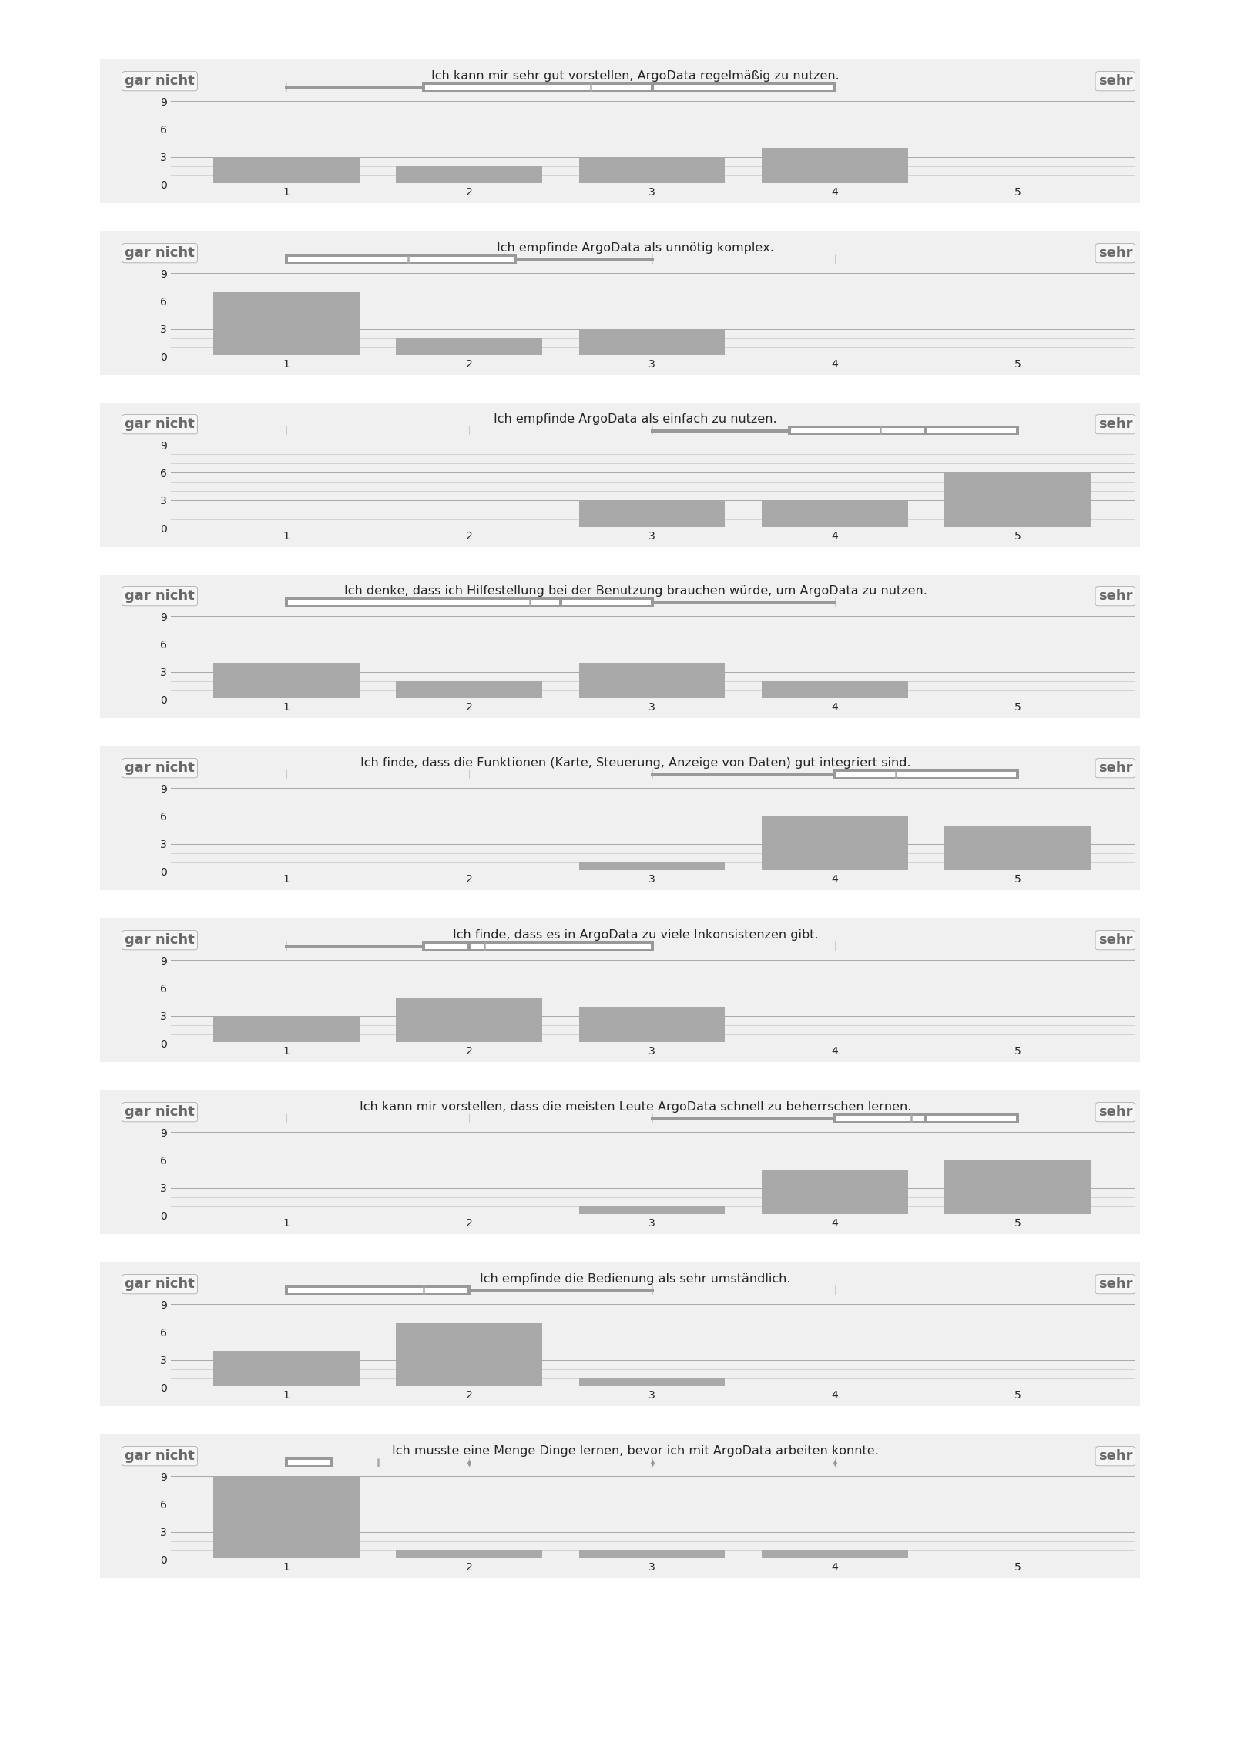
\includegraphics[width=\textwidth,height=0.98\textheight,clip=true,trim=2cm 3cm 1.6cm 1cm]{pix/surveyAuswertung.pdf}

 \label{fig:surveyAuswertung}
 \caption{Ergebnis der Umfrage zur Usability}
\end{figure}

\section{Demonstration und Auswertung}


\begin{figure}[H]
 \centering
 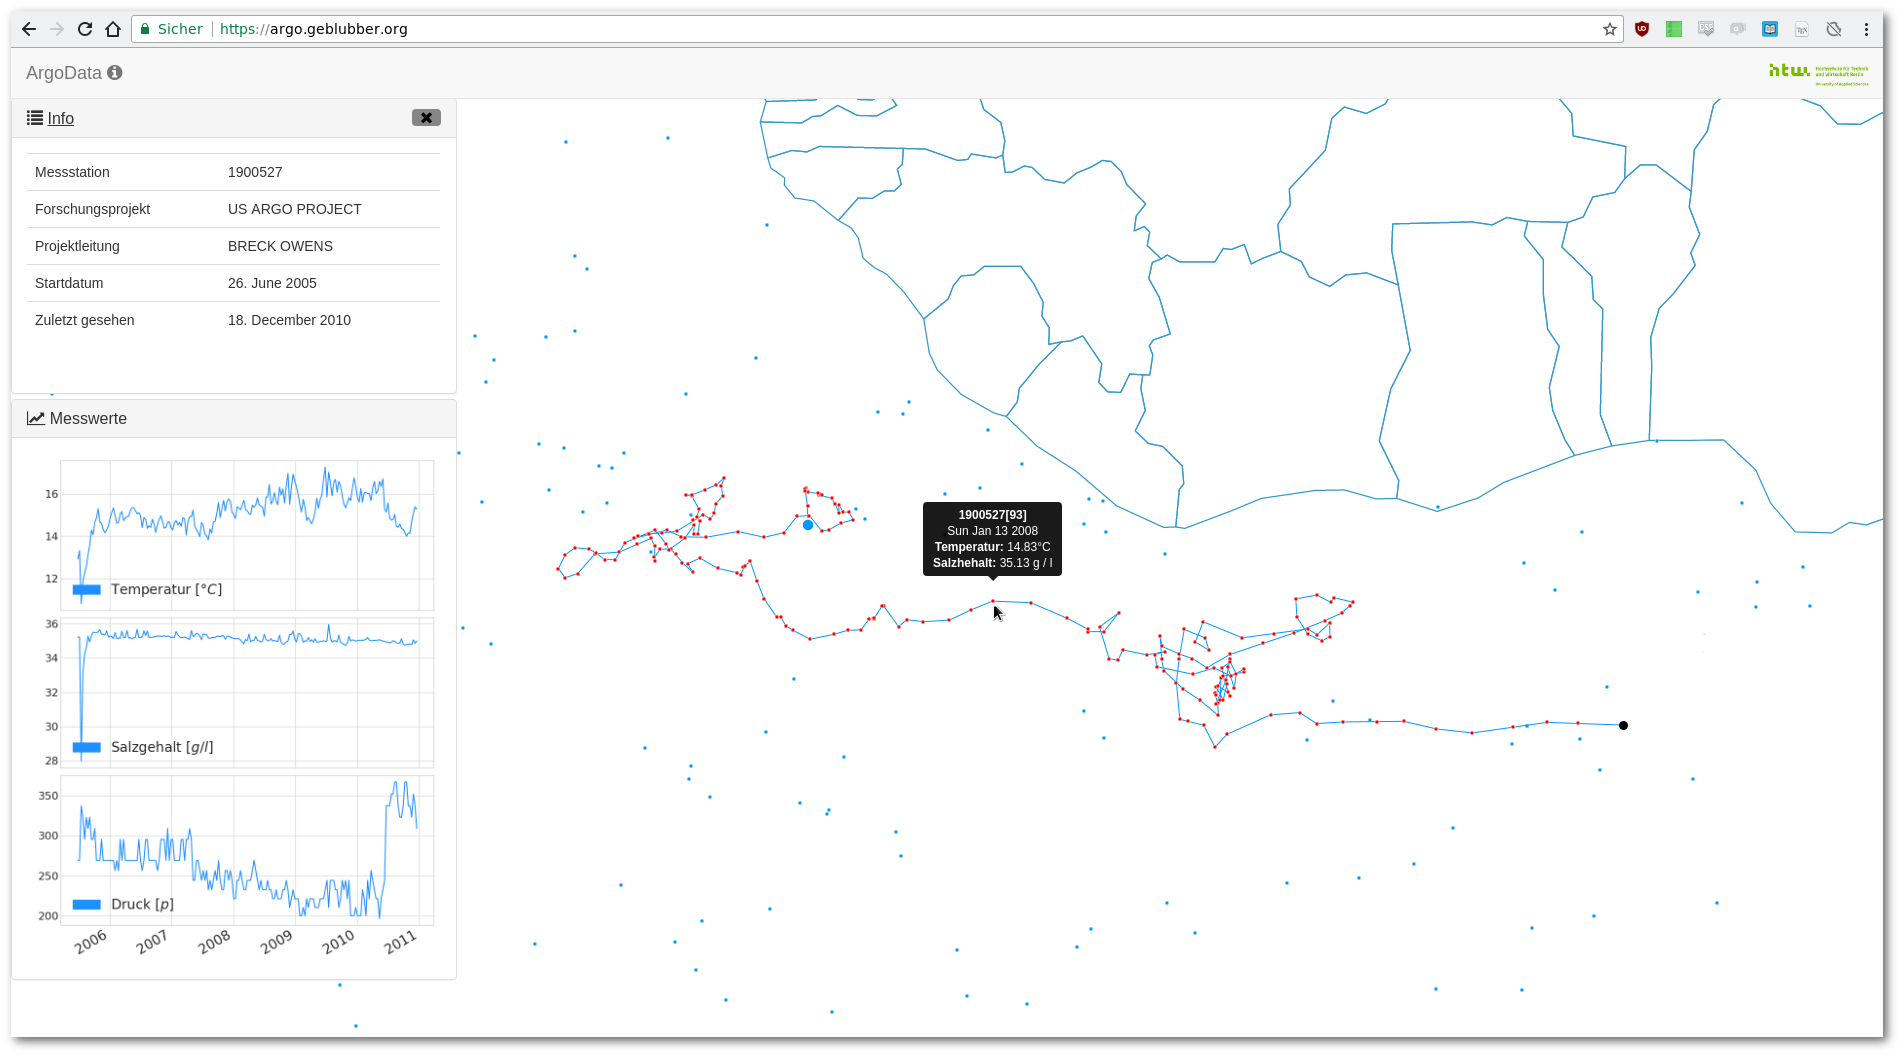
\includegraphics[width=\textwidth]{pix/argodata_complete.png}
 % argodata_complete.png: 1872x1026 px, 96dpi, 49.52x27.14 cm, bb=0 0 1404 769
 \caption{Die Webpräsenz von Argo-Data}
 \label{fig:argodataWeb}
\end{figure}




Damit endet diese Arbeit mit folgendem Zitat aus dem Buch "`\textit{Zen und die Kunst ein Motorrad zu warten}"' von Robert M. Pirsing:

\begin{quotation}
 Der echte Zug des Wissens ist nichts Statisches, das man anhalten und in Teile zerlegen kann. Er ist immer in Fahrt. Auf einem Gleis namens Qualität. Und die Lok und die 120 Güterwagen fahren nie woanders hin, als wo das Gleis der Qualität sie hinführt.
\end{quotation} 


\pagebreak
\pagestyle{plain}\pagenumbering{roman}\setcounter{page}{6}
\bibliography{bib.bib}
\bibliographystyle{alpha}
\nocite{*}

\pagebreak


\section{Anhang}

\section*{Resultate}

\subsection*{Daten aus der SUS Umfrage}

\begin{tabular}{l||rrrrrrrrrrrr}
\toprule
\textbf{User-Index} &  0  &  1  &  2  &  3  &  4  &  5  &  6  &  7  &  8  &  9  &  10 &  11 \\
\midrule
\textbf{Statement 1} &   4 &   3 &   2 &   3 &   1 &   4 &   3 &   2 &   1 &   4 &   1 &   4 \\
\textbf{Statement 2}         &   1 &   2 &   2 &   1 &   3 &   1 &   1 &   3 &   3 &   1 &   1 &   1 \\
\textbf{Statement 3}       &   4 &   3 &   5 &   5 &   3 &   5 &   5 &   3 &   4 &   5 &   5 &   4 \\
\textbf{Statement 4} &   1 &   4 &   1 &   3 &   2 &   4 &   1 &   3 &   3 &   3 &   1 &   2 \\
\textbf{Statement 5} &   4 &   4 &   4 &   5 &   3 &   5 &   5 &   4 &   4 &   5 &   4 &   5 \\
\textbf{Statement 6} &   3 &   2 &   3 &   2 &   2 &   2 &   1 &   3 &   3 &   2 &   1 &   1 \\
\textbf{Statement 7} &   4 &   4 &   5 &   5 &   4 &   5 &   5 &   3 &   4 &   4 &   5 &   5 \\
\textbf{Statement 8}  &   2 &   2 &   2 &   2 &   1 &   2 &   1 &   2 &   3 &   1 &   2 &   1 \\
\textbf{Statement 9} &   4 &   5 &   5 &   4 &   4 &   4 &   5 &   3 &   2 &   5 &   4 &   4 \\
\textbf{Statement 10} &   1 &   1 &   1 &   3 &   1 &   1 &   1 &   2 &   4 &   1 &   1 &   1 \\
\bottomrule
\end{tabular}


\subsection*{Erzeugung der Umfragegraphen}

\begin{python}
import numpy as np
import seaborn as sns
import matplotlib.pyplot as plt
import matplotlib.patches as patches
from matplotlib.ticker import AutoMinorLocator
from matplotlib.font_manager import FontProperties

plt.style.use('fivethirtyeight')

def subplot(data):
    bins=[1,2,3,4,5]
    y = [data.value_counts()[x] if x in data.value_counts() else 0 for x in bins]

    f, (ax_box, ax_hist) = plt.subplots(2, sharex=True, gridspec_kw={"height_ratios": (.1, .86)})
    f.set_figwidth(20)
    f.set_figheight(2.3)

    whisker = sns.boxplot(data.values, 
                          ax=ax_box,showmeans=True, 
                          meanline=True, color="white", 
                          meanprops=dict(color='darkgrey', linestyle='-', linewidth=2.5,))
    ax_hist.bar(bins, y, color="darkgrey")
    ax_box.set(yticks=[])

    sns.despine(ax=ax_hist)
    sns.despine(ax=ax_box, left=False)

    f.suptitle(data.name, fontsize=16)   
    
    left, width = -.06, 1
    bottom, height = -0.09, .33
    right = left + width
    top = bottom + height
    p = patches.Rectangle(
        (left, bottom), width, height,
        fill=False, transform=ax_hist.transAxes, clip_on=False
    )
      
    font = FontProperties()
    font.set_weight('bold')
    font.set_size(18)  
    bbox = dict(facecolor='whitesmoke', edgecolor='grey', pad=0.2, boxstyle='round')
    ax_hist.text(right, height, 'sehr',
        horizontalalignment='center',
        verticalalignment='top',
        transform=ax.transAxes,
        fontproperties=font,
        color = 'dimgray',
        backgroundcolor='whitesmoke', 
        bbox=bbox)
    ax_hist.text(left, height, 'gar nicht',
        horizontalalignment='center',
        verticalalignment='top',
        transform=ax.transAxes,
        fontproperties=font,
        color = 'dimgray',
        backgroundcolor='whitesmoke', 
        bbox=bbox)
    
    plt.yticks(np.arange(0, 9+1, 3.0))
    ax_hist.set_ylim([0,9])
    ax_hist.minorticks_on()
    ax_hist.xaxis.grid(False)
    ax_hist.yaxis.grid(b=False, which='minor', color='lightgray', linestyle='-')
    ax_hist.yaxis.set_minor_locator(AutoMinorLocator(3))
    ax_hist.yaxis.grid(b=True, which='major', color='darkgray', linestyle='-', markersize=1)
    ax_box.xaxis.grid(True)    

for col in df:
    subplot(df[col])
\end{python}

\subsection*{Erzeugen des Anforderungsgraphen}


\begin{python}
import networkx as nx
from networkx.drawing.nx_agraph import write_dot, graphviz_layout
import pandas as pd
import numpy as np
import matplotlib.pyplot as plt
from matplotlib.patches import Rectangle
import matplotlib.patches as mpatches
import matplotlib.patches
from matplotlib import pylab
URL_DOC =   "https://docs.google.com/spreadsheets/d/e/2PACX-1vQfFMHK_XVtNXex5pAPh6boF4qdBH0iB6_ndGWV"\
            "-FANyBXh1TB9MuIQ_Ex7gBlcrGOMO2Tn133NxVf1/pub?gid=0&single=true&output=csv"

color_map = {
  'kann': 'tomato',
  'soll': 'orange',
  'muss': 'green'
}

anforderungen = pd.read_csv(URL_DOC)

unpack = lambda cell: [c[1:-1] for c in cell.split("|")]

anforderungen_ = [row['Titel'] for i, row in anforderungen.iterrows()]
nachbedingungen_ = [unpack(row['Nachbedingungen']) for i, row in anforderungen.iterrows()]
vorbedingungen_ =  ["" if pd.isnull(row['Vorbedingungen']) else unpack(row['Vorbedingungen']) for i, row in anforderungen.iterrows()]

flat_nachbedingungen = [item for sublist in nachbedingungen_ for item in sublist]
flat_vorbedingungen = [item for sublist in nachbedingungen_ for item in sublist]


G = nx.DiGraph()
G.add_nodes_from(anforderungen_)
G.add_nodes_from(flat_nachbedingungen)

A = G.subgraph(anforderungen_)
N = G.subgraph(flat_nachbedingungen)

for i, a in enumerate(anforderungen_):
    for n in nachbedingungen_[i]:
        G.add_edge(n,a, weight=1000)
    for v in vorbedingungen_[i]:
        G.add_edge(a,v, weight=0.0001)

G = G.reverse()
A = A.reverse()
n = N.reverse()

pos=graphviz_layout(G, prog='dot')

plt.figure(3,figsize=(36,40))
plt.axis('off')

color = [color_map[row['Prioritaet']] for i, row in anforderungen.iterrows()]

nx.draw_networkx_nodes(A, pos, node_shape='s', node_size=10000, node_color=color, alpha=0.6, label=True)
nx.draw_networkx_nodes(N, pos, node_shape='o', node_size=200, node_color='grey')
nx.draw_networkx_edges(G, pos, node_shape='o')

x_centr = np.average([p[0] for p in pos.values()])

fontsize = 10

def shift_x(x):
    align_map = {
        -1: 'left',
        1: 'right'
    }
    s = 1 if x < x_centr else -1
    return (align_map[s], x - (s*7))

def shift_y(y):
    return (y + 20)

def position_string(node):
    x,y = pos[node]
    align, x = shift_x(x) if False in N else ('center', x)
    y = y-10 if  node in N else y
    y = shift_y(y) if node in A else y
    return (align,x,y)

for n in G:
    align,x,y = position_string(n)

    plt.text(x,y,s=n, bbox=dict(facecolor='lightgray', alpha=0.5),
             horizontalalignment=align,
             color='black', fontsize=27)
plt.rcParams["legend.fontsize"] = 22
plt.legend(handles=[
    mpatches.Patch(color=color_map['muss'], label='Prioritaet: muss'),
    mpatches.Patch(color=color_map['kann'], label='Prioritaet: kann'),
    mpatches.Patch(color=color_map['soll'], label='Prioritaet: soll'),
    mpatches.Ellipse((1,1), 4, 0, fill=True, label='Nachbedingung', color='grey')
])
plt.show()
\end{python}


\pagebreak
\printnoidxglossaries


\end{document}
